\documentclass[Main.tex]{subfiles}

\begin{document}


\section[Analisi qualitativa della dinamica]{Analisi qualitativa delle equazioni differenziali ordinarie dei sistemi newtoniani}

\toc

\newpage
\subsection{Introduzione}
Le equazioni differenziali ordinarie del primo ordine sono le più  importanti della meccanica, perché ogni problema è riducibile alla risoluzione di questa equazione. 

Si possono scrivere come:
\begin{equation}
	\ddot x = \frac{1}{m}f(x) := g(x)
\end{equation}
O anche col sistema del primo ordine
\begin{equation}
	\begin{cases}
	\dot x =v \\
	\dot v = g(x)
\end{cases}
\end{equation}

Questo sistema è sostanzialmente uguale ai casi affrontati precedentemente, infatti è del tipo $\dot Y=F(Y)$ dove per $Y=(x,v)$, e quindi $F(Y)$ è un campo vettoriale in 2D (nello spazio delle fasi $(x,v)$).


Questi sistemi (equazione di Newton su $\mathbb{R}$ con forza posizionale) sono conservativi, infatti come già fatto vedere precedentemente la quantità
\begin{equation}
	H= \frac{m}{2} \dot x^2 + U(x)
\end{equation}
è costante lungo le soluzioni dell'equazione di Newton. Dove $U'(x) = -f(x)$ (ovvero $U(x) =- \int f(x) dx$) è l'energia potenziale della forza esterna $f(x)$.

\begin{dm}
\begin{gather}
	\dot H = \frac{d}{dt}(H(x(t), \dot x(t))) = m \dot x \ddot x +U'(x) \dot x=\\
	\dot x (m \ddot x + U'(x)) = \dot x (m \ddot x - f(x))=0
\end{gather}
e quindi $H$ si conserva e lungo il moto vale:
\begin{equation}
	H(x,\dot x)= H(x_0,v_0)= \frac{m}{2} v_0^2 + U(x_0)
\end{equation}
\end{dm}

\newpage
\begin{osservazioni}

	\item Il sistema generale di equazione differenziali ordinarie autonome in $\mathbb{R}^2$ è della forma:

\begin{equation}
	\begin{cases}
	\dot x = A(x,v)\\
	\dot v = B(x,v)
\end{cases}, \ \left(\begin{array}{c}
x \\
v
\end{array} \right)  \in \Rr^2
\end{equation}

E di conseguenza i sistemi meccanici (conservativi) sono una sottoclasse molto particolare di questi con $A(x,v)=v$.

	\item È interessante notare come si possa arrivare allo stesso risultato anche moltiplicando per $\dot x$ l'equazione di Newton\footnote{è come se stessimo ricavando un'espressione della potenza}:
\begin{equation}
	\dot x m \ddot x = \dot x f(x) =-\dot x \frac{dU(x)}{dx}= - \frac{d}{dt}U(x)
\end{equation}
Dove $\dot x m \ddot x = \frac{d}{dt}\frac{m}{2} \dot x^2$, e quindi portando tutto a sinistra:

\begin{equation}
  \frac{d (K+U)}{dt}=\frac{d H}{dt}=0
\end{equation}

Questo procedimento ha il vantaggio che introduce in modo naturale la quantità $H$ senza conoscerla a priori.
\end{osservazioni}

\newpage
\subsection{Diagrammi di fase}
Esistono soluzioni costanti che sono delle coppie del tipo $(\tilde x,0)$, e si ricavano in modo analogo a prima ponendo $F(Y)=0$ e di conseguenza si ha che le soluzioni costanti/di equilibrio sono:
\begin{equation}
  t \mapsto (x(t),v(t))=(\tilde x,0) \ \forall t
\end{equation}
invece da un punto di vista energetico questi corrispondono alle coppie $(\tilde x, 0)$ tale che l'integrale primo $H$ sia minimo, che alla fine dei conti corrisponde al trovare al trovare i minimi di $U(x)$. Inoltre siccome $H$ si conserva lungo il moto, quest'ultimo deve necessariamente svolgersi sugli insiemi di livello di $H$:

\begin{equation}
  H(x(t),v(t)) = E \ (=H(x_0,v_0))
\end{equation}
Cioè le curve $t \mapsto \left( \begin{array}{c} x(t) \\ v(t)\end{array} \right) $ soluzioni di $\begin{cases} \dot x= v \\ \dot v = \frac{1}{m}f(x)\end{cases}$ giacciono su un insieme di livello $H$ determinato dalle condizioni iniziali.

Si chiama \emph{piano della fasi}, o \emph{ spazio di fase}, o \emph{spazio della fasi}. Per $n$ punti materiali che si possono muovere in $R^d$, lo spazio delle delle fasi ha dimensione $2\cdot n \cdot d$. In questo caso si ha che:
\begin{df}
Il grafico di $f(x)$ con il verso delle traiettorie del sistema e dei punti di equilibrio si chiama \emph{diagramma di fase} dell'equazione $\dot x = f(x)$.
\end{df}



Per il moto unidimensionale (cioè un solo punto che si muove sulla retta $\Rr$ soggetto alla $f(x)$) l'insieme di livello è costituito da curve piane, eventualmente degeneri in un punto, oppure è vuoto.
\begin{figure}[H]
    \centering
    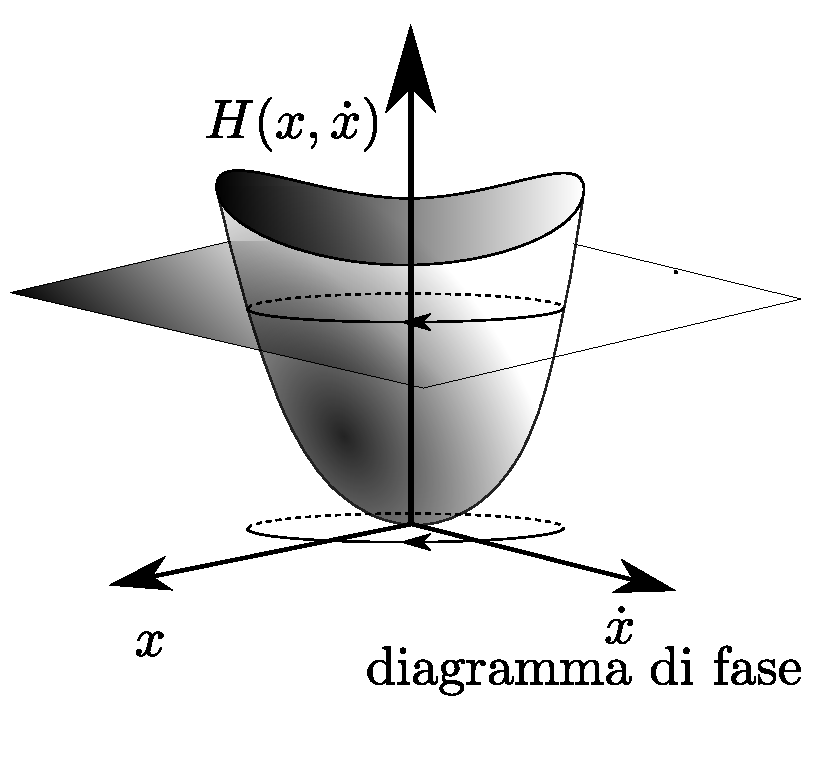
\includegraphics[width=0.5\columnwidth]{images/insieme_di_livello.pdf}
\end{figure}

\newpage
\begin{osservazioni}
	\item Nei casi che si studieranno si avrà l'espressione esplicita di $H$, quindi ovvero si ha un'equazione che identifica esattamente le curve di livello:
\begin{gather}
	\frac{m}{2} \dot x^2 +U(x) =E\\
	\rightarrow \dot x ^2 = \frac{2}{m} (E - U(x))\\
	\rightarrow \dot x = \pm \sqrt{\frac{2}{m}(E-U(x))} \ \ \ \ (U(x) \leq E)
\end{gather}
Quindi le curve di livello, dette anche \textit{orbite} nello spazio delle fasi $(x,v)$, sono delle curve simmetriche rispetto all'asse $x$. Quindi sostanzialmente basta disegnare la curva di livello all'energia $E=H(x_0,v_0)$ e il punto si muoverà su tale curva con velocità $(v,\frac{f(x)}{m})$ e il moto vero e proprio avviene sull'asse $x$ ottenuto proiettando il moto 2D che avviene sulla curva di livello. 

\item È importante sottolineare la seguente cosa:
\begin{equation}
  K= \frac{m\dot x ^2}{2}  \geq 0 \rightarrow \frac{m \dot x^2}{2}= E-U(x) \geq 0 \rightarrow U(x)\leq E
\end{equation}


Il valore dell'energia potenziale $U(x)$ non può superare il valore dell'energia $E$ come mostrato sopra\footnote{alla fine è ciò che dice la conservazione dell'energia, cioè che la somma dell'energia cinetica e potenziale è fissata, questo modo di pensare semplifica e rende evidenti molte cose successive.}, quindi il moto vero può avvenire soltanto su degli intervalli dell'asse $x$ che sono soluzione della disequazione scritta sopra.

\end{osservazioni}


\newpage
\subsection{Come disegnare un diagramma di fase}
Più in generale per disegnare un ritratto di fase, si disegna $U(x)$ e fissato un certo livello di energia si trova l'intervallo di $x$ in cui il moto è permesso, basta prendere l'intervallo di $\Rr$ dove la $U(x)<E$.

\begin{figure}[H]
    \centering
    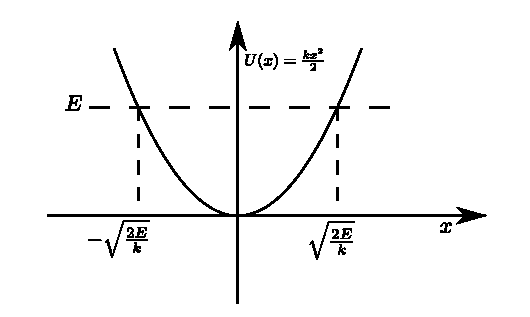
\includegraphics[width=0.4\textwidth]{images/diagramma.pdf}
\end{figure}

 Si trova che la $x$ deve essere compresa tra i due \emph{punti di inversione}, chiamati così  perché quando $U = E$ allora $K=0$ e di conseguenza anche la velocità è nulla e c'è dunque l'inversione del moto.
 Più  in generale si disegna il grafico di $U(x)$ e sotto si tiene il grafico x-v. Si trovano i punti di inversione che rappresentato gli estremi della curva di livello. Se il numero dei punti di inversione è due allora ci sarà una curva chiusa e simmetrica rispetto all'asse $x$ che li collega e ha tante gobbe quante ne ha $U(x)$ (bisgona ricordare che la somma tra $U(x)$ e $K$ è fissata ad $E$). Se il numero dei punti inversione (diverso dal punto di equilibrio) è uno allora la curva sarà aperta e andrà ad infinito. 
 
 \begin{figure}[H]
    \centering
    \includegraphics[width=0.4\textwidth]{images/diagramma2.pdf}
\end{figure}

\newpage
\subsection{Analisi locale vicino a un punto di minimo}
In un caso più  complesso si può avere:

\begin{figure}[H]
    \centering
    \includegraphics[width=0.6\textwidth]{images/diagramma3.pdf}
\end{figure}

Per risolvere questo caso si può procedere con la
\emph{linearizzazione del sistema Newtoniamo vicino a $r(E_{min})$.}
Sopra si è mostrato che per un'equazione differenziale lineare autonoma le curve di livello sono delle ellissi esatte, invece cosa accade se il sistema non è lineare? Accade una cosa simile, cioè si aprono delle curve chiuse simili a ellissi vicino ai punti di equilibrio. È possibile vederlo linearizzando l'equazione differenziale, infatti ragionando come nel caso di equazioni $\dot x=f(x)$ si pone $(x(t),\dot r(t))=(r_*,0)+(\xi,\eta)$ segue che:
\begin{equation}
  \begin{cases}
x(t) =r_* + \xi(t)\\
\dot r(t)=0+ \eta(t)
\end{cases}
\end{equation}
derivando e sostituendo nell'equazione differenziale originale:
\begin{equation}
  \begin{cases}
	\dot \xi = \eta\\
	\dot \eta = - \frac{1}{m}  U'(r_* + \xi)
\end{cases}
\end{equation}
ora invece sfruttando il fatto che ci si trova in un punto dello spazio delle fasi vicino al punto di equilibrio $(r_*,0)$ si può calcolare lo sviluppo di Taylor attorno a tale punto:
\begin{equation}
  \begin{cases}
	\dot \xi = \eta\\
	\dot \eta = -\frac{1}{m} \left[U' (r_*) + U''(r_*) \xi + ... \right]
\end{cases}
\end{equation}
siccome si è vicino a un punto di equilibrio semplice/non degenere ($\frac{d^2 U(r_*)}{dx^2}\neq 0$), si ha:
\begin{equation}
  \begin{cases}
	\dot \xi = \eta\\\
	\dot \eta = - \frac{1}{m} U'' (r_*) \xi
\end{cases}
\iff \ddot \xi = - \omega ^2 \xi 
\end{equation}
con  $w:=\sqrt{\frac{U''(r_*)}{m}}$. Il sistema scritto sopra è lineare in $(\xi,\eta)$ e riconduce all'equazione dell'oscillatore armonico che ha una soluzione già nota:
\begin{equation}
  t \mapsto \begin{cases}
 \xi(t)=a \cos (\omega t) + b 	\sin (\omega t)\\
 \eta(t)= - \omega a \sin(\omega t) + \omega b \cos(\omega t)
 \end{cases}
\end{equation}
tutto questo è perchè si è appunto approssimato $U(x)$ con una parabola vicino al suo punto stazionario $r_*$. Questa è anche la descrizione parametrica dell'ellisse nello spazio delle fasi, e quindi il moto è periodico di periodo $\frac{2 \pi}{\omega}$

\begin{figure}[H]
    \centering
    \includegraphics[width=0.6\textwidth]{images/Diagrammafase.pdf}
\end{figure}

\newpage
\begin{osservazioni}
	\item Tra i punti di inversione il moto è regolare e monotono (cioè sulla curva di livello ci si muove in un verso senza fermarsi), in particolare si trovano i punti critici (le gobbe delle curve di livello menzionate prima) con lo studio della conservazione dell'energia:
\begin{equation}
  v_{\pm} (x) = \pm \sqrt{\frac{2}{m} (E-U(x))} \longrightarrow \text{considerando  $v_+(x)$} \longrightarrow
\end{equation}
\begin{equation}
  \frac{d}{dx}v_+(x) = \frac{-\frac{2}{m}U'(x)}{2 \sqrt{\frac{2}{m}(E-U(x))}} = - \frac{1}{m} \frac{U'(x)}{\sqrt{\frac{2}{m}(E-U(x))}}
\end{equation}
Come già detto prima, $U(x)$ e $v_+(x)$ hanno le gobbe allineate, quando una ha un minimo l'altra un massimo e viceversa.

\item Supponendo che il moto avvenga su una curva chiusa nello spazio delle fasi, qual è il tempo di percorrenza tra $x_+$ e $x_-$ (i due punti di inversione)? Come già visto:

$$v_+=  \dot x= + \sqrt{\frac{2}{m}(E-U(x))}$$
e separando le variabili:

$$
\longrightarrow dt = \frac{dx}{\sqrt{\frac{2}{m} (E-U(x))}}
$$
integrando tra $x_-(E)$ e $x_+(E)$ si ottiene il periodo completo:
\begin{equation}
T= 2 \int_{x_-(E)}^{x_+(E)} \frac{dx}{\sqrt{\frac{2}{m}(E-U(x))}}
\end{equation}
L'integrando esiste sempre continuo nell'intervallo considerato, tranne agli estremi dove presenta qualche problema. 

Queste due osservazioni sono trattate più in dettaglio per il caso del potenziale kepleriano \underline{\ref{Ukepleriano}}.
\end{osservazioni}


\newpage
\subsection{Analisi locale vicino a un punto di minimo, caso radiale}
In modo del tutto analogo è possibile sviluppare lo stesso ragionamento nel caso del moto centrale in cui $U$ dipende da $r$. Lo sviluppo di questo calcolo è incentrato nel determinare l'equazione per $\theta(t)$. Si considera come prima $r_*$ il valore di $r$ relativa al valore minimo di energia $E_*$ e si immagina di perturbarla di un valore $\Delta E >0$ tale che $\frac{\Delta E}{E}\ll 1$. In tal caso Vale che

\begin{equation}
  E=E_* \Rightarrow r(t) = r_* \ \forall \ t  \Rightarrow \dot \theta = \frac{\ell_z}{ \mu r_*^2}
\end{equation}
Cioè si ha un moto circolare uniforme. Per valore di energia $E>E_*$ si ha un moto radiale limitato dai punti di inversione $r_+$ e $r_-$.

	\subsubsection*{Conservazione dell'energia}
	
	\begin{equation}
		 \frac{\mu \dot r^2}{2} + U_e(r) = E = E_*+ \Delta E
	\end{equation}
	sviluppando l'energia efficace attorno ad $r_*$ si ha:
	
	\begin{gather}
		U_e(r) = U_e(r_*) + \cancel{U'_e(r_*) (r-r_*)} + \frac{1}{2} U_e'' (r_*) (r-r_*)^2 + o(3)\\
		= E_* + \frac{1}{2} U_e''(r_*) (r-r_*)^2+o(3)
	\end{gather}
	Dove $U'=0$ perchè si sta studiando un punto di minimo.
	
	\begin{equation}
		\frac{\mu \dot r^2}{2} + \cancel{E_*} + \frac{1}{2} U_e''(r_*) (r-r_*)^2 + o(3) = \cancel{E_*} + \Delta E
	\end{equation}
	La quale si può riscrivere come:
	\begin{gather}
		\frac{U'' (r-r_*)^2}{2 \Delta E} + \frac{\mu \dot r^2}{2 \Delta E} = 1+ o \left( \frac{(r-r_*)^3}{\Delta E} \right)\\
		= \frac{(r-r_*)^2}{\frac{2 \Delta E}{U''}} + \frac{\dot r^2}{\frac{2 \Delta E}{\mu}} = 1+ o \left( \frac{3}{\Delta E} \right)
	\end{gather}
	cioè l'equazione di un'ellisse centrata in ($r_*,0$) con semiasse dell'ordine di $\sqrt{\Delta E}$
	
	\newpage
	\subsubsection*{Equazione del moto}
	
	\begin{equation}
		\mu \ddot r= - U_e'(r)
	\end{equation}
	Definendo $\xi:= r-r_*$ si ha $r(t)=r_* + \xi(t)$
	\begin{equation}
		\Rightarrow \mu \ddot \xi = - U_e'(r_* + \xi ) = \cancel{- U_e'(r_*)} - U_e''( r_*) \xi + o(\xi ^2)
	\end{equation}
	Ovvero l'equazione dell'oscillatore armonico che risolta da:
	\begin{equation}
		r(t) = r_* + \xi(t) = r_* + a \cos ( \omega t ) + b \sin (\omega t) + o ( \Delta E)
	\end{equation}
	con $\omega^2 = \frac{U_e''(r)}{\mu} >0$.
	
	\subsubsection*{Ricostruzione del moto spaziale}
	
	\begin{equation}
		\dot \theta = \frac{\ell_z}{\mu r^2(t)} = \frac{\ell_z}{\mu ( r_* + \xi(t))^2} = \frac{\ell_z}{ \mu r_*^2\left(1 + \frac{\xi(t)}{r_*}\right)^2}
	\end{equation}
	Dato che per costruzione $\frac{\xi(t)}{r_*} \ll 1$ si può sviluppare secondo Taylor: 
	\begin{gather}
		\frac{1}{1+ \epsilon} = 1- \epsilon + \epsilon^2 + ... \Rightarrow \frac{1}{(1+ \epsilon)^2} = 1 + 3 \epsilon^2 - 2 \epsilon +...\\
		\Rightarrow \boxed{\theta(t) = \frac{\ell_z}{\mu r_*^2}t - \frac{2 \ell_z}{\mu r_*^2}\int_0^t \xi(s) ds + \frac{3 \ell_z}{\mu r_*^4}\int_0^t \xi ^2(s) ds + o(\xi^3)}
	\end{gather}


\newpage
\subsubsection{Due esempi importanti di potenziale}

\begin{tema}[Potenziale armonico]
	Utilizzando la legge di conservazione dell'energia che per l'oscillatore armonico si ha:
\begin{equation}
		H(x, \dot x) = \frac{m \dot x^2}{2} + \frac{k x^2}{2}
\end{equation}

%(-(x)= - kx= f(x))

Si studiano gli insiemi di livello di tale funzione\footnote{Essendo questa una funzione da $\Rr^2$ a $\Rr$ è possibile rappresentarla in $\Rr^3$ come una superficie, gli insiemi di livello $E$ equivale a tagliare la superficie all'altezza $E$ e prendere la sezione che ne risulta (una curva)}:

\begin{equation}
	H(x,\dot x) = E
\end{equation}

Detto in altro modo si intende insieme di livello $E$ di $H$ l'insieme 
\begin{equation}
	S:= \{(x, \dot x) \in \mathbb{R}^2 : H(x, \dot x) = E \} = H^{-1}(E)
\end{equation}


Inoltre si può notare che la funzione $H$ è non negativa in tutto $\Rr^2$, quindi non esistono gli insiemi di livello per $E<0$.
Invece per gli altri casi si distinguono i seguenti casi:
\begin{itemize}
\item \textbf{E > 0} $$
\frac{kx^2}{2} + \frac{m \dot x^2}{2}=E
$$
Ora si potrebbe isolare $\dot x$ per averla in funzione di $x$, ma conviene scriverla in tale modo:
$$
\frac{x^2}{2E/k} + \frac{\dot x^2}{2E/m}=1
$$
Cosicché questa risulta essere l'equazione di un'ellisse di semiassi $\sqrt{\frac{2E}{k}}$ e $\sqrt{\frac{2E}{m}}$


\begin{figure}[H]
	\centering 	
	\hspace{2cm} 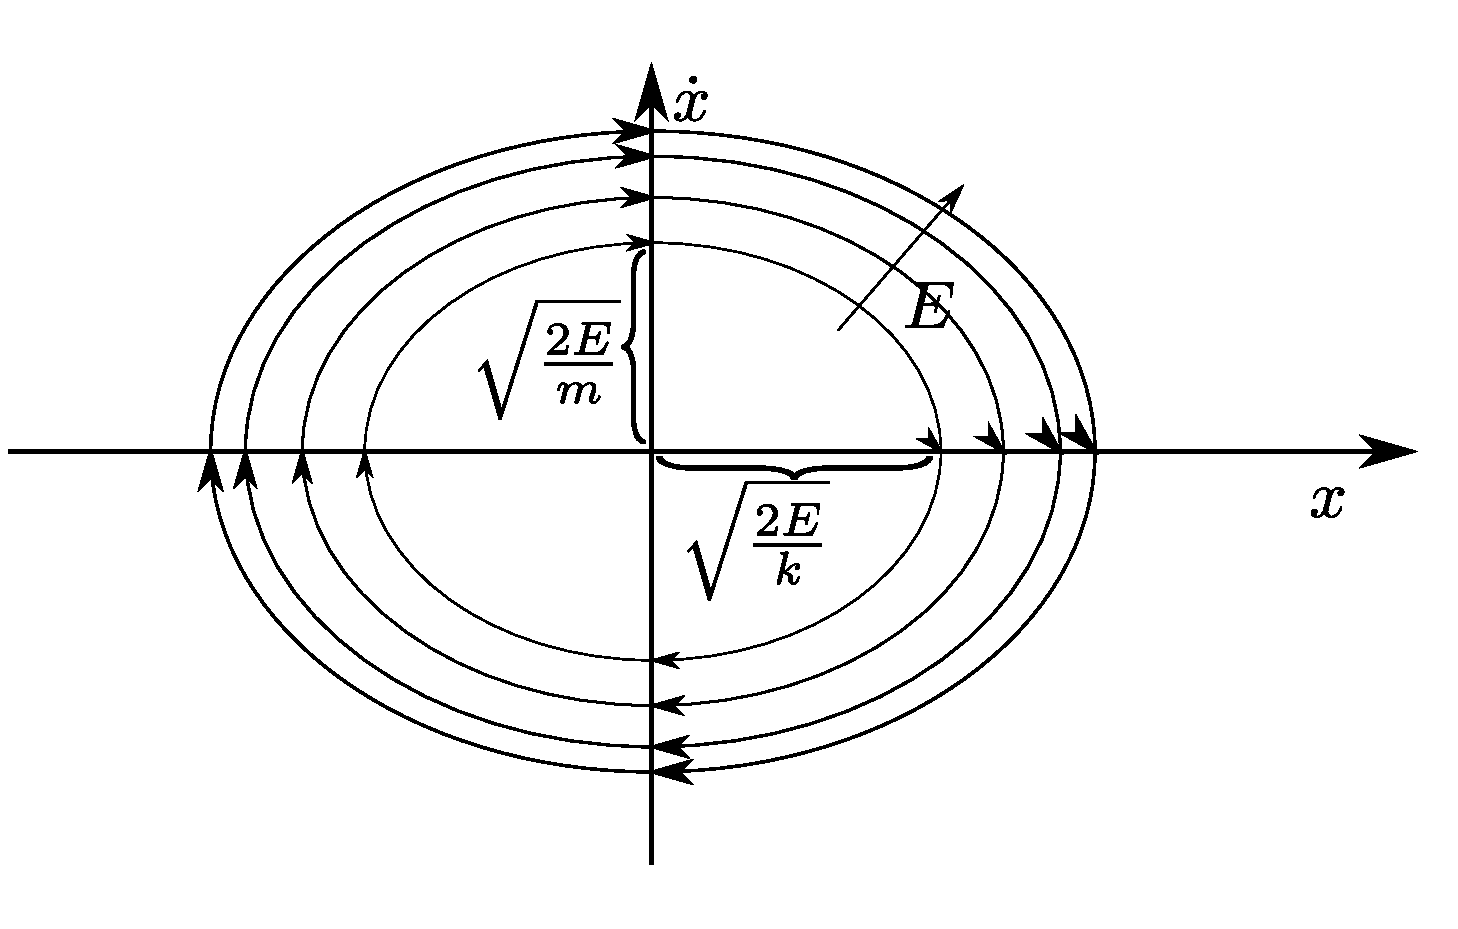
\includegraphics[width=0.7\textwidth]{images/ellisse.pdf}{}
\end{figure}

  	
Inoltre quando si disegna il diagramma di fase nello spazio delle fasi $(x,\dot x)$ bisogna indicare tutti i versi di percorrenza delle curve di livello. Quindi scelta una curva di livello basta prenderne un punto che sta sopra l'asse $x$ e il verso è sempre da sinistra verso destra. Una banale conseguenza è che le orbite chiuse sono sempre percorse in senso orario.

\item \textbf{E=0}
$$E=0 \iff x=0, \ \dot x=0$$

Ovvero un punto di equilibrio (l'unico) del sistema, cioè l'origine del piano $(x,\dot x).$ Quindi al diminuire di E le ellissi degenerano nel punto di origine.
\end{itemize}

\begin{comment}
In modo alternativo si può scrivere l'energia nella forma:
\begin{equation}
	\frac{\mu \dot r^2}{2} + \frac{\ell_z^2}{2 \mu r^2}-\frac{k}{r}
\end{equation}

Il potenziale efficace è della forma:
\begin{equation}
	U'_e(r)= - \frac{\ell_z^2}{\mu r^3} +kr =0 \Rightarrow r_c = \left( \frac{\ell_z^2}{\mu k }\right)^\frac{1}{4} = \frac{ |\ell_z|^\frac{1}{2}}{\left( \mu k \right)^\frac{1}{4}}
\end{equation}
L'energia minima invece si trova cercando il minimo di $U_e(r)$
\begin{equation}
	E_{min}= \min_{r>0} U_e(r) = U_e(r_c) = \frac{\ell_z^2 \sqrt{\mu k}}{2 \mu |\ell_z|} + \frac{1}{2} k \frac{|\ell_z|}{\sqrt{\mu k}} = r_c^2 = \frac{|\ell_z|}{\sqrt{\mu k}}= \sqrt{\frac{k}{\mu}} | \ell_z|
\end{equation}
\end{comment}
\end{tema}

\newpage
\begin{tema}[Potenziale kepleriano] \label{Ukepleriano}
	Vale la pena notare che è raro che i potenziali valgano strettamente, per esempio per studiare il moto della Terra rispetto al Sole, oltre alle influenze degli altri pianeti, ci sono altre correzioni legate al fatto che i corpi non sono puntiformi, hanno una struttura interna\footnote{cosa che viene completamente ignorata nel concetto della particella}, etc.: $U(r)_{\text{corr}}:= \frac{k}{r} (1+...)$. Anzi più in generale il potenziale potrebbe non essere proprio più dipendente dalla sola $r$.

	La formulazione dell'energia è
	\begin{equation}
	H= \frac{\mu \dot r^2}{2} + U_e(r) =E \longrightarrow \frac{\mu \dot r^2}{2}=E-U_e(r) \geq 0
\end{equation}
Gli intervalli consentiti di moto radiale sono quelli dell'insieme \{$r>0: \ U_e(r) \leq E$\}. In generale se $U_e$ ammette un minimo assoluto ed $E_{min}=\min_{r>0} U_e(r)$ allora per $E<E_{min}$ non si hanno moti.
Inoltre dalla legge di conservazione $\dot \theta = \frac{\ell_z}{\mu r^2}$

\begin{equation}
	U_e(r) = \frac{\ell_z^2}{2 \mu r^2} - \frac{k}{r}
\end{equation}
Se $U_e(r)=0 \Rightarrow r_0 = \frac{\ell_z^2}{2 \mu k}$
\begin{equation}
	U'_e(r) =0 \iff - \frac{\ell_z^2}{\mu r^3} + \frac{k}{r^2} =0 \Rightarrow r_c = \frac{\ell_z^2}{\mu k} (= 2 r_0)
\end{equation}

Serve un disegno qualitativo. Ha una sola radice per la derivata, quindi c'è un punto critico e calcolando i valori asintotici per $x \rightarrow 0$ (tende a $+\infty$) e $x \rightarrow + \infty$ (tende a 0) si vede che è per forza un punto di minimo; chiamato $r_c$. È possibile disegnarne il grafico.
 

\begin{itemize}
	\item $\mathbf{E=E_{min}}$ 
	
	Aumentando l'energia, il primo livello energetico interessante si incontra per $E=U_e( r_c)$.  L'unico valore di $r$ consentito è quindi $r_c$, essendo costante si può determinare la legge del moto per $\theta$.
\begin{equation}
	\dot \theta = \frac{\ell_z}{\mu r_c^2} \Longrightarrow \boxed{\theta (t) = \theta (0) + \underbrace{ \frac{\ell_z}{\mu r_c^2}}_{\omega_c} t}
\end{equation}
Ovvero moto circolare uniforme nello spazio fisico. Di conseguenza si può ricavare il periodo $T=\frac{ 2\pi}{\omega}$. \bigskip


\item $\mathbf{E_{min}<E<0}$

Invece per energie superiori, ma comunque sotto lo zero, si aprono delle (specie di) ellissi attorno a $r=r_c$ dando due punti di inversione $r_+$ e $r_-$. Si possono trovare calcolando le radici di 
\begin{gather}
	\frac{\ell_z^2}{2 \mu r^2}- \frac{k}{r} =E \longrightarrow \frac{\ell_z^2}{2\mu} - kr = Er^2 \\
	\rightarrow r^2 + \frac{k}{E}r - \frac{\ell_z^2}{2 \mu E}=0 \Rightarrow \boxed{r_\pm = \frac{1}{2} \left[ - \frac{k}{E} \pm \sqrt{\frac{k^2}{E^2} + \frac{4 \ell_z^2}{2 \mu E}} \right]} \notag
\end{gather} 
La condizione della radice impone che $E_{min}<E<0 \Rightarrow 0<r_- <r_+$
Ciò significa che il moto è limitato nello spazio fisico e quindi per il teorema di Bertrand sono anche chiuse: il caso corrisponde a delxle ellissi per il moto reale. 


\item $\mathbf{E=0}$

Invece per $E=0$ si ha una parabola come moto nello spazio fisico, e per energie superiori si trovano delle iperboli. Quest'ultime non sono curve limitate quindi il corpo esce dall'influenza gravitazionale per $t \rightarrow +\infty$. Inoltre la curva di fase per $E=0$ è detta \emph{separatrice} tra i due tipi moto. 
\end{itemize}
Per capire il verso di percorrenza si basti pensare che quando $\dot r>0$ vuol dire che $r$ sta crescendo, quindi va verso destra. Viceversa, quando $\dot r<0$ allora $r$ sta diminuendo, quindi va verso sinistra. Il grafico del potenziale e del moto radiale nel piano $(r, \dot r)$ è quello riportato.

\begin{figure}[H]
	\centering 	
	\hspace{80pt} 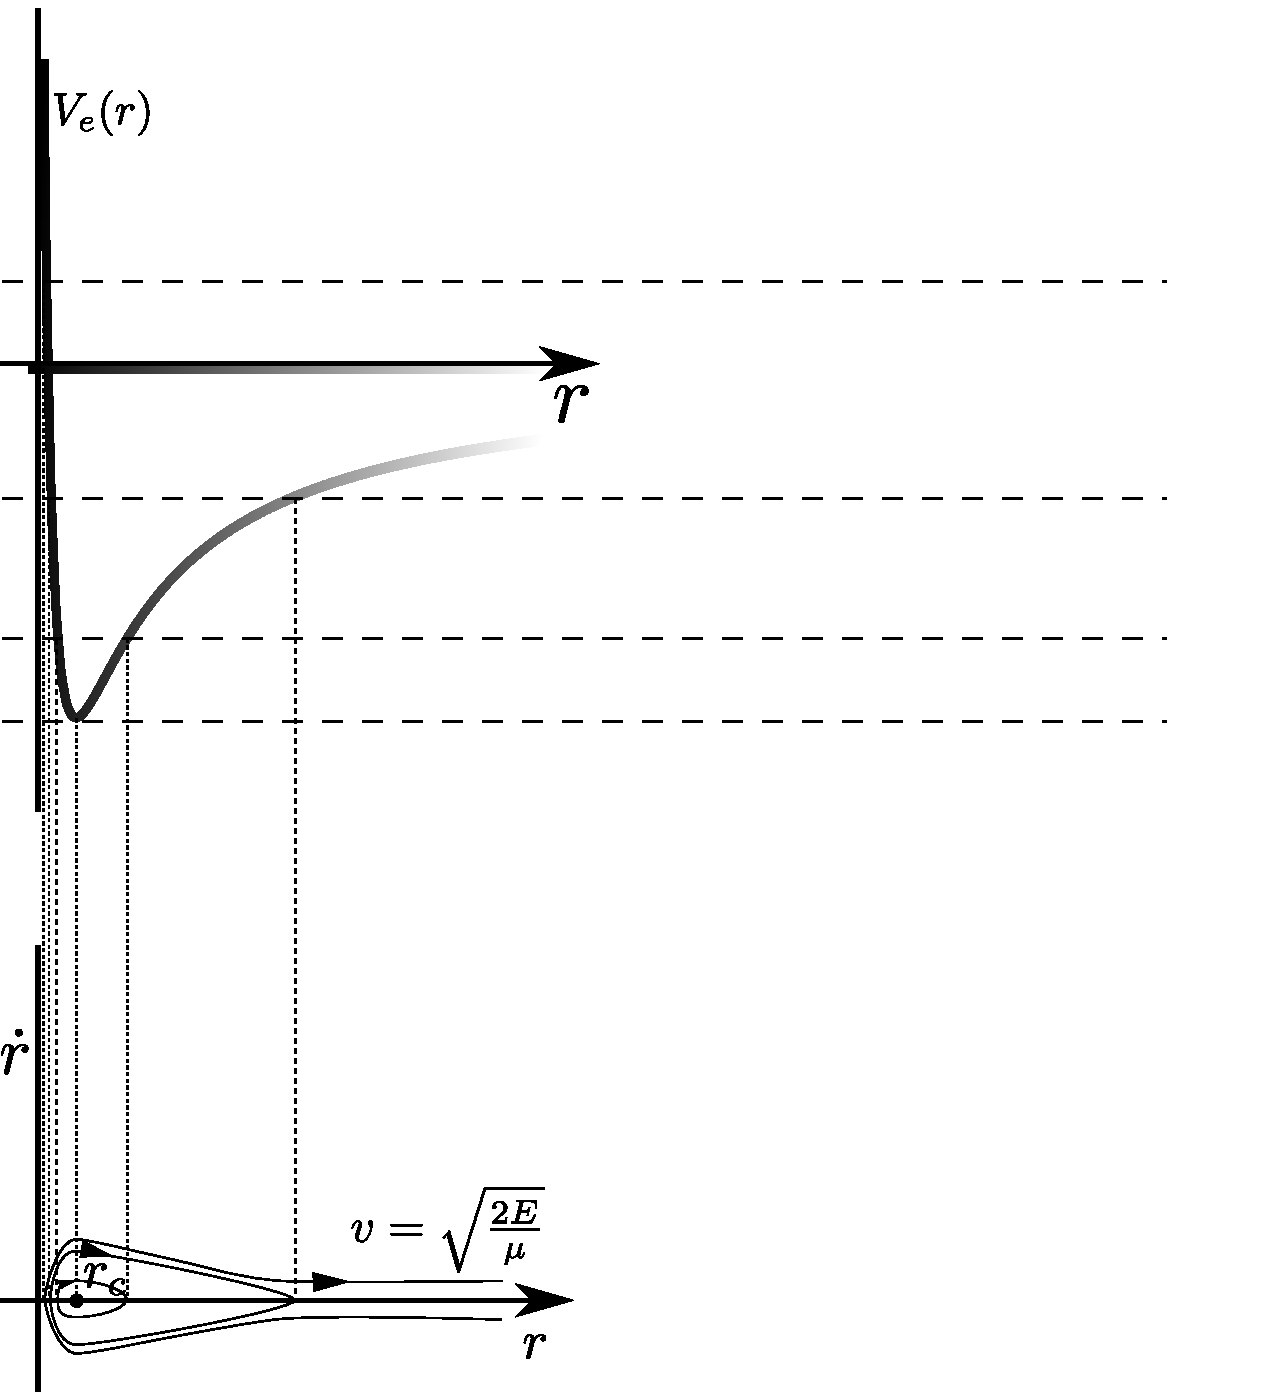
\includegraphics[width=0.9\textwidth]{images/keplero.pdf}{}
\end{figure}



\begin{osservazioni}
	\item L'orbita poteva avere un'altra forma pur mantendendo il massimo centrale e i due zeri $r_-$ e $r_+$? Siccome 
	\begin{gather}
		\dot r = + \sqrt{\frac{2}{\mu} (E-U_e(r))}\\
		\dd{\dot r}{r} = \frac{-\frac{2}{\mu} E'_e(r)}{2 \sqrt{\frac{2}{\mu} (E-U_e(r))}}\overset{?}{=}0
	\end{gather}
	Che è $0$ dove si annulla il numeratore, cioè dove si annulla $U'_e(r)$ cioe $r_c$. Inoltre la funzione è monotona crescente per $r_-<r<r_c$ e monotona decrescente per $r_c<r<r_+$. 
	
	\item Bisogna verificare anche che non ci siano punti angolosi (cosa non scontata vista la presenza della radice), per vedere ciò si calcolano i limiti per $r \rightarrow r_\pm$ da destra e sinistra. Da destra si ha:
	\begin{equation}
		\lim_{r \rightarrow r_-^+}\dd{\dot r}{r}= - \frac{U'_e(r)}{\sqrt{2 \mu (E-U_e(r)}}= + \infty
	\end{equation}
	In questo caso il numeratore resta finito nel calcolo del limite perchè $U'(r_-)$ non è un punto critico. Da sinistra ci si aspetta $- \infty$ affinché ci sia continuità. Ed è così. Le condizioni imposte sono:
	\begin{equation}
		\dd{\dot r}{r} \rightarrow \pm \infty \text{ per } r \rightarrow r_\mp^\pm
	\end{equation} 
	\item Lo spazio fisico $(r, \theta)$ è diverso da quello del diagramma di fase $(r, \dot r)$ in cui sono contenute le informazioni del moto radiale.
\end{osservazioni}
\end{tema}


\newpage
\begin{tema}[Moto di stelle nelle galassie e di galassie negli ammassi]
	Si consideri un ammasso sferico di materia con densità $\rho(s)$ dove $s$ è la distanza dal centro; di raggio $R$ oltre al quale non c'è niente.
L'energia potenziale $U(r)$ dell'ammasso sferico è della forma:
\begin{equation}
	U(r)= -Gm   2 \pi \int_{0}^{R} \rho(s) s^2 \left( \int_0^\pi \frac{\sin \theta d \theta}{ \sqrt{r^2 + s^2 - 2rs \cos \theta}} \right) ds 
\end{equation}
Dove il fattore $2 \pi$ è il risultato dell'integrazione in $d \varphi$. Per risolvere si applica la sostituzione $u= - \cos \theta$
\begin{gather*}
	= - \pi Gm \int_0^R \rho(s) s^2 \int_{-1}^1 \frac{du}{\sqrt{s^2 +r^2 +2rsu}} ds =\\
	=- \pi Gm \int_0^R \rho(s) s^2 \left( \left. \frac{\sqrt{s^2 + r^2 + 2rs u}}{rs} \right|_{u=-1}^{u=1} \right) ds=\\
=- 2 \pi \frac{Gm}{r} \int_0^R \rho (s) s \left( r+ s - |r-s| \right)ds=\\
\Rightarrow U(r)=\begin{cases}
		- \frac{Gm}{r} \underbrace{\left( 4 \pi \int_0^R \rho(s) s^2 ds \right)}_{M} \ \ &r>R\\
	- 2 \pi  \frac{Gm}{r} \left[ \int_0^r \rho(s)s 2s ds  + \int_r^R \rho(s) s \cdot 2r ds \right] &0<r<R
\end{cases}
\end{gather*}
Concentrandosi sul caso $0<r<R$ si ha:
\begin{equation}
	- 4 \pi \frac{Gm}{r} \left[ \int_0^r \rho(s) s^2 ds + r \int_r^R \rho(s) s ds \right]
\end{equation}
Adesso, se $\rho(s)$ è indipendente da $s$ si può portare fuori dall'integrale:
\begin{gather*}
	\Rightarrow U(r) = - 4 \pi \frac{Gm}{r} \rho \left[ \frac{r^3}{3} + \frac{r}{2} (R^2-r^2) \right]= \\
	= - 4 \pi \frac{Gm}{r} \rho \left( - \frac{1}{6} r^3 + \frac{1}{2} R^2r \right) = \boxed{\frac{2 \pi}{3} Gm \rho r^2 - 2 \pi Gm \rho R^2}
\end{gather*}
Che ha la forma dell'equazione di un oscillatore armonico $U(r) \sim r^2$, bisogna sottolineare che è stato approssimata la distribuzione della galassia come se fosse continua.
Il risultato ottenuto è che 
\begin{equation} \label{potenzialeammasso}
	U(r)= \begin{cases}
 	- \frac{GmM}{r} \ \ &r>R\\
 	\frac{2 \pi}{3} Gm \rho r^2 - 2 \pi Gm \rho R^2 &r<R
 \end{cases}
\end{equation}
Andando a calcolare la forza del potenziale si ha:
\begin{equation} \notag
	F(r)= -U'(r)= \begin{cases}
 	- \frac{GmM}{r^2} \ \ &r>R\\
 	- \frac{4 \pi}{3} Gm \rho r = - \frac{G \left( \frac{4}{3}\pi r^3 \rho \right) m}{r^2}=-\frac{GM(r) m}{r^2} &r<R
 \end{cases}
\end{equation}
\begin{wrapfigure}{l}{0.35\textwidth}
	\includegraphics[width=0.35\textwidth]{images/darkmatter} \caption*{\scriptsize{Velocità radiale osservata della galassia NGC 3198 confrontata con la curva di rotazione prevista dai dati fotometrici. Il grafico in alto mostra la densità di massa del disco. \\ Fonte: Begeman, K.G., "HI rotation curves of spiral galaxies. I. NGC 3198," Astronomy and Astrophysics, Vol. 223, p. 47-60, 1989.}}\vspace{-1cm}
\end{wrapfigure}
Passando allo studio qualitativa si ha che il potenziale efficace è della forma:
\begin{equation}
	U_e(r) = \frac{\ell_z^2}{2mr^2} +U(r)
\end{equation}
Dove $U(r)$ è \eqref{potenzialeammasso}, quindi all'interno si hanno orbite circolari infatti $U(r)=cr^2$ esplicitando $\ell_z= mr^2 \dot \theta = m r v_\theta$ dove $v_\theta = r \dot \theta$. Il moto circolare si ha 
\begin{gather*}
	U'_e(r)=0 \iff - \frac{\ell_z^2}{mr^3} + 2cr = 0 \\ \Rightarrow \frac{m^2 \cancel{r^2} \dot r^2_\theta}{r^{\cancel{3}}}=2cr
\end{gather*}


\noindent Da qua si trovano i valori di $v_\theta$ nei due casi:
\begin{equation*}
	\begin{cases}
		v_\theta (r)= \text{cost} \cdot r \ \ & r<R\\
		- \frac{m^2 v_\theta^2}{mr} + \frac{GmM}{r^2}=0 \Rightarrow v_\theta =  \text{cost} \frac{1}{\sqrt{r}} &r>R
	\end{cases}
\end{equation*}

\

Quindi per $r$ interni la velocità è costante mentre fuori va come $\sim r^{-\frac{1}{2}}$.

C'è una discrepenza con i dati sperimentali perchè risulta che per $r>R$ la velocità non decresce come $\sim \frac{1}{\sqrt{r}}$ ma è costante. Sembrerebbe che ci fosse materia (quindi massa) che non hanno un'interazione elettromagnetica e quindi sfuggono all'analisi degli esperimenti. Questo è il problema della materia oscura e consiste circa nel 90\% della massa presente. 

%TODO sistemare in case di book layout
 Tuttavia si può notare che se la densità di materia oscura fosse della forma:
\begin{align*}
	\rho_{dark}(s) = \frac{k}{s^2} \rightarrow U(r) &= - \frac{ \text{cost}}{r} \left[ r+ r \log R - r\log r \right] \\ &=  \text{cost} + \text{cost} \log r
\end{align*}

Il potenziale sarebbe allora logaritmico e la derivata è $1/r$ che cancella esattamente il termine che fa discostare l'esperimento dalla teoria.
\end{tema}



\newpage
\subsection{Analisi locale vicino a un punto di massimo}
Per quanto riguarda il massimo locale, supponendo che $r_*$ sia massimo locale non degenere di $U(r)$ e cioè:
\begin{gather} \notag
	U_e(r) = U_e(r_*) + U'_e(r_*)(r-r_*) + \frac{1}{2} U_e''(r_*)(r-r_*)^2+o(3)\\
	E=E_* + \Delta E \ \ \ \ \ \ E_*=U_e(r_*)
\end{gather}
Dalla conservazione dell'energia:
\begin{equation}
	\frac{\dot r^2}{2} = U_e(r) = \frac{\dot r^2}{2} + \cancel{E_*} + \frac{1}{2} U_e'' (r_*)(r-r_*)^2 + o(3) = \cancel{E_*} + \Delta E
\end{equation}
Per semplificare le notazioni si può definire tutto in funzione di $|\Delta E|$ e usando la funzione segno per dargli il segno:

\begin{equation}
  \Delta E = \sigma | \Delta E | \ \ \ \ con \ \sigma = sgn( \Delta E) = \pm 1
\end{equation}
E quindi riprendendo l'equazione di prima e facendo qualche semplificazione e la nuova notazione si ha:
\begin{equation}
  \frac{\dot r^2 }{2} - \frac{|U'(r_*')|}{2} (r-r_*')^2+... = \sigma |\Delta E|
\end{equation}
E mettendo in forma normale:
\begin{equation}
  \frac{\dot r^2}{2 |\Delta E|} - \frac{(r-r_*')^2}{2 | \Delta E| / |U''(r_*')|} - ... = \sigma
\end{equation}
Nel caso in cui $\sigma=+1$ si ha:
\begin{equation}
  \begin{cases}
	\sigma= + 1 \longrightarrow (\Delta E>0)\\
	\frac{\dot r^2}{b^2} - \frac{(r-r_*')^2}{a^2} = +1
\end{cases}
\end{equation}
cioè l'equazione di un'iperbole (entrambi i rami).

Analogamente per $\sigma = -1$ si ha:
\begin{equation}
  \begin{cases}
	\sigma= - 1 (\Delta E<0)\\
	-\frac{\dot r^2}{b^2} + \frac{(r-r_*')^2}{a^2} = +1
\end{cases}
\end{equation}
che è l'equazione dell'altra iperbole (i due rimanenti rami) con gli stessi asintoti dell'iperbole precedente.

Man mano che ci si avvicina con l'energia al massimo locale di $U(r)$ ($E= U_e'(r_*),\ (\Delta E =0)$), i due rami dell'iperbole degerano in due asintoti. L'equazione degli asintoti si trova riprendendo l'equazione dove non si è ancora fatto la divisione per $\Delta E$ e lo si pone uguale a 0:
\begin{equation}
  \dot r^2 = |U'(r_*')|(r-r_*')^2 \Longrightarrow
  \dot r= \pm \sqrt{|U'(r_*')|}(r-r_*')
\end{equation}
Nel centro dell'iperbole si ha il punto di eq. instabile $(r_*',0)$ e quest'ultimo è il punto di incontro degli asintoti costituendo così un punto angoloso per la curva di livello che si raccorda agli asintoti. 

Sempre riferendosi alla stessa figura ci sono tre tipi di moti possibili date dalle soluzione dell'equazione: vicino ai punti di equilibrio stabili si aprono curve chiuse simili a ellissi che ad un certa energia si raccordano agli asintoti dando origine alle connessione omocline (collegano un punto di equilibrio a se stesso), aumentando ancora l'energia si trovano delle curve a otto.

\begin{figure}[H]
    \centering
    \includegraphics[width=0.9\textwidth]{images/curvaotto.pdf}
\end{figure}

Quindi concludendo i punti di equilibrio $(\tilde r ,0)$ corrispondenti ai minimi locali non degeneri dell'energia potenziale ($U'( \tilde r) = 0 , U'' (\tilde r) >0$) si chiamano centri.
\\ I punti di equilibrio $(\tilde r ,0)$ corrispondenti a massimi locali non degeneri dell'energia potenziale ($U'(\tilde r)=0, U''(\tilde r) <0$) si chiamano punti iperbolici o punti di sella.

\newpage
\begin{tema}[Orbita di Mercurio, problema dei tre corpi] 
Il potenziale per il problema dei tre corpi, che è stato ricavato analiticamente nel tema \ref{es:6}, è della forma:
\begin{gather} \notag
	U_{medio} ( \xi, t) = - Gm_J \left( \frac{1}{|x|} + \frac{1}{4} \frac{|\xi|^2}{|x|^3} + ... \right)+ \\-Gm_S \left( \frac{1}{|\xi|} + \frac{\mu^2}{4} \frac{|x|^2}{|\xi|^3} +...\right) \notag
\end{gather}
Riscrivendo il potenziale con $|x|:=R$
\begin{equation}\notag
	U_{medio} (\xi,t)=- \frac{Gm_S}{|\xi|} - \frac{Gm_S \mu^2}{4} \frac{R^2}{|\xi|^3} + \frac{G m_J }{4} \frac{|\xi|^2}{R^3} \left( -\frac{Gm_S}{R} \right)
\end{equation}
Il primo termine è la forza di gravitazione già vista, poi compare un termine che va come l'inverso del cubo di $\xi$ cioè un potenziale attrattivo, dominante per $\xi$ piccoli. L'effetto fisico di quest'ultimo è superiore rispetto al potenziale centrifugo che va come l'inverso del quadrato di $\xi$. 

Il termine ultimo è un potenziale repulsivo armonico, è presente perchè Giove attira gravitazionalmente Mercurio e quello è il risultato medio.	

\begin{osservazione}
	Le sorti di Mercurio sembrerebbero quindi due, o il Sole lo attira fino a inglobarlo, o Giove lo allontana completamente dal campo gravitazionale del Sole. Per chiarire ciò si può valutare il rapporto tra i due termini pertubativi:

\begin{gather*}
	\cancel{G} m_J  \frac{|\xi|^2}{R^3} \frac{1}{\cancel{G}m_S \mu^2} \frac{|\xi|^3}{R^2} = \frac{1}{\mu} \left( \frac{|\xi|}{R} \right)^5 \\ \simeq 10^3 \left( \frac{ 0.4 }{5} \right)^5 \simeq 10^3 \cdot 10^{-5} = 10^{-2} \ll 1
\end{gather*}
Quindi il contributo dominante è quello del Sole. Questo rapporto sottolinea l'importanza di non essersi fermati allo sviluppo di dipolo nel calcolo analitico del potenziale.
\end{osservazione}
\begin{gather}
	\ddot \xi = - \pp{U_{medio}}{\xi},  \ \ \ \ U_{medio}= U_{medio}(|\xi|)\\
	\Rightarrow \ell = \xi \times \dot \xi \ \text{costante}\\
	\boxed{H = \frac{|\dot \xi|^2}{2} + U_{medio} ( |\xi|)}
\end{gather}
Passando alle coordinate polari nel piano di $\xi$
\begin{gather}
	\ell_z=r^2 \dot \theta  \ \ \ \ \ |\dot \xi|^2 = \dot r^2 + \dot r \dot \theta^2 = \dot r^2 + \frac{\ell_z^2}{r^2}\\
	\boxed{H = \frac{\dot r^2}{2} + \underbrace{\frac{\ell_z^2}{2r^2}+ U_{medio}(r)}_{U_e(r)}=E}
\end{gather}
I valori di $r$ consentiti sono per valori di $U_e(r) \leq E$.
Per poter disegnare il potenziale si scrive l'espressione esplicita del potenziale efficace $U_e(r)$:
\begin{equation}
	U_e(r) = \underbrace{\frac{\ell_z^2}{2r^2} - \frac{Gm_S}{r}}_{\text{Potenziale ordinario kepleriano}} - \frac{Gm_S \alpha}{r^3} - Gm_J Kr^2
\end{equation}
Con $\alpha= \frac{\mu^2R^2}{4}$ e $k=\frac{1}{4R^3}$. 
Il grafico del potenziale, confrontato con il potenziale kepleriano è:

\begin{figure}[H]
    \centering
    \includegraphics[width=0.8\textwidth]{images/PotenzialeMercurio.pdf}
\end{figure}


Come è chiaro dal grafico, a differenza del caso kepleriano imperturbato, l'analisi del ritratto di fase prende in considerazione anche i due punti di massimo introdotti rispettivamente dal termine $\sim r^{-3}$ dovuto alla presenza del sole (primo massimo) e dal termine $\sim r^2$ dovuto dalla presenza  dovuto alla presenza di Giove. Si riporta di seguito il ritratto di fase.

\begin{figure}[H]
    \centering
    \includegraphics[width=0.7\textwidth]{images/mercurio.pdf}
\end{figure}

\subsubsection{Precessione del perielio vicino all'orbita circolare}
Scrivendo ora il potenziale efficace trascurando il termine quadratico in $r$ perchè è piccolo rispetto agli altri, si ha:
\begin{equation}
	U_e(r) = \frac{\ell_z^2}{2r^2} - \frac{Gm_S}{r} - \frac{Gm_S \alpha}{r^3}
\end{equation}
Dove $\alpha= \frac{\mu^2 R^2}{4}$ e $\mu = \frac{m_J}{m_S}$.

L'obbiettivo è calcolare, attorno il minimo, il moto di precessione. Innanzitutto si cerca il minimo
\begin{equation}\notag
	U_e'(r)= - \frac{\ell_z^2}{r^3} + \frac{Gm_s}{r^2} + \frac{3Gm_S \alpha}{r^4}=0\Rightarrow \boxed{r^2 - \frac{\ell_z^2 }{Gm_S}r + 3 \alpha=0}
\end{equation}
Gli zeri sono:
\begin{equation}
	r_\pm = \frac{1}{2} \left[ \underbrace{\frac{\ell_z^2}{Gm_S}}_{r_K} \pm \sqrt{\left( \underbrace{\frac{\ell_z^2}{Gm_S}}_{r_K} \right)^2 -12 \alpha} \right]
\end{equation}
Dove $r_K$ è il raggio dell'orbita kepleriana non perturbata. La condizione di esistenza, dalla radice, di $r_\pm$ è 
\begin{equation}
	\exists \ r_\pm : \ \ell_z^2 \geq Gm_S \sqrt{12 \alpha} = \sqrt{3}Gm_S \mu R
\end{equation} 
In termini di $r_K$ la condizione è equivalente a $r_K > \sqrt{3} \mu R$ che è ampiamente verificata nel caso reale dell'orbita di Mercurio. Altrimenti il potenziale centrifugo non è sufficiente a modificare la forma del potenziale efficace che diventa monotono crescente.

%TODO immagine potenziale senza effetto centrifugo

Riscrivendo la derivata del potenziale 
\begin{equation}\notag
U_e'(r)=\frac{Gm_S}{r^4} \left( r^2 - \frac{\ell_z^2}{Gm_S}r + 3 \alpha \right) = \frac{Gm_S}{r^4} (r-r_+)(r-r_-)
\end{equation}
Si vede subito che $r_-$ è punto di massimo e $r_+$ di minimo senza aver calcolato la derivata seconda ma solo fattorizzando.
\begin{osservazione}
	Se $r_c=r_+ \rightarrow \frac{\ell_z^2}{Gm_S}$ si ha il caso kepleriano.
\end{osservazione}

\newpage
Attorno al minimo locale $r_c$ l'orbita è circolare. considerando l'equazione
\begin{gather*}
	\ddot r = - U_e'(r) \\ r(t) =r_c + \xi (t) \Longrightarrow \ddot \xi = - U_e''(r_c) \xi \\
	\omega_{rad} = \sqrt{U_e''(r)} \Rightarrow T_{rad} = \frac{2 \pi }{ \omega_{rad}} = \frac{ 2 \pi}{ \sqrt{U_e''(r_c)}}\\
	\dot \theta = \frac{\ell_z}{r^2} \Rightarrow \Delta \theta (T_{rad}) = \frac{\ell_z}{r_c^2}T_{rad} = \boxed{ \frac{\ell_z}{r_c^2} \frac{ 2 \pi}{ \sqrt{U_e''(r)}}}
\end{gather*}
Dove ci si aspetta che 
\begin{equation}
	\frac{\Delta \theta (T_{rad})}{2 \pi} = \frac{\ell_z}{r^2_c} \frac{1}{\sqrt{U_e''(r)}}
\end{equation}
 In questo caso $U_e(r) = \frac{\ell_z^2}{2r^2}+U(r)$ perchè $U(r) = - \frac{Gm_S}{r} - \frac{Gm_s \alpha}{r^2}$. Siccome $r_c$ è definito a partire da $U'_e(r)=0$ cioè
 \begin{equation}
 	- \frac{\ell_z^2}{r^3} + U'(r)=0 \Rightarrow \frac{\ell_z^2}{r^3} = U'(r)
 \end{equation}
 Per $r=r_c$ vale che $U''_e(r) = \frac{3 \ell_z^2}{r^4} + U''(r) \underset{\underset{r=r_c}{\uparrow}}{=} \frac{3}{r} U'(r) + U''(r)$
 cioè
 \begin{equation}
 	\boxed{ U_e''(r_c) = \frac{3}{r_c} U'(r_c) + U''(r_c)}
 \end{equation}
Inoltre  $\frac{|\ell_z|}{r_c^2} = \sqrt{\frac{U'(r_c)}{r_c}} $  allora:
\begin{equation*}
	\frac{\Delta \theta (T_{rad})}{2 \pi} = \frac{\sqrt{U'(r_c)/r_c}}{\sqrt{3 \frac{U'(r_c)}{r_c} + U''(r_c)}}= \frac{1}{\sqrt{3 + r_c U''(r_c)/U'(r_c)}}
\end{equation*}
Ci si è ricondotti a un'equazione dove compaiono le derivate, fino alla seconda, dell'energia potenziale:
\begin{flalign} \notag
	&U(r) = - \frac{Gm_S}{r} - \frac{Gm_S \alpha}{r^3} = - Gm_s \left( \frac{1}{r} + \frac{\alpha}{r^3} \right)\\
	&U'(r) = Gm_S \left( \frac{1}{r^2} + \frac{3 \alpha}{r^4} \right)\\
	&U''(r) = -Gm_S \left( \frac{2}{r^3} + \frac{12 \alpha}{r^5} \right)
\end{flalign}
Da qua è possibile ottenere 
\begin{gather*}
	\Rightarrow \frac{rU''(r)}{U'(r)} = \frac{- \cancel{Gm_S} \left( \frac{r}{r^2} + \frac{12 \alpha}{r^4} \right)}{\cancel{Gm_S} \left( \frac{1}{r^2} + \frac{3 \alpha}{r^4} \right)} = - \frac{2r^2 + 12 \alpha}{r^2 + 3 \alpha}\\
	\Rightarrow \frac{\Delta \theta (T_{rad})}{2 \pi} = \frac{1}{\sqrt{3 - \frac{2 r_c^2 + 12 \alpha}{r^2_c +3 \alpha}}}=
	\boxed{ \sqrt{\frac{r_c^2 + 3 \alpha}{r_c^2- 3 \alpha }}}
\end{gather*}
Riscrivendo ora $r_c$ si ha
\begin{gather}
	r_c= r_+= \frac{1}{2} \left( r_k + r_k \sqrt{1- \frac{12 \alpha}{r_K^2}} \right)=\\
	= r_K \left( \frac{1 + \sqrt{1- 12 \alpha /r_K^2}}{2} \right) \underset{\underset{ \frac{12 \alpha}{r_K^2} \ll 1}{\uparrow}}{=}\\
	\simeq r_K \left( \frac{1+ 1 - \frac{6 \alpha}{r_K^2}}{2} \right) = r_K \left( 1- \frac{3 \alpha}{r_K^2}\right)
\end{gather}
E il suo quadrato è quindi
\begin{gather}\notag
	r^2_c = r_K^2 \left( 1 - \frac{3 \alpha}{r_K^2} \right)^2 = r_K^2 \left( 1- \frac{6 \alpha}{r_K^2} + O\left( \frac{\alpha^2}{r_K^4} \right) \right) \simeq r^2_K - 6 \alpha
\end{gather}

\newpage
\begin{gather*}
	\frac{\Delta \theta (T_{rad})}{2 \pi} = \left( \frac{r_K^2 - 6 \alpha + 3 \alpha}{r_K^2 - 6 \alpha - 3 \alpha} \right)^\frac{1}{2} = \sqrt{ \frac{r_K^2 - 3 \alpha}{r^2_K - 9 \alpha}} =\\
	= \frac{\sqrt{1- 3 \alpha/r_K^2}}{\sqrt{1- 9 \alpha /r_K^2}} = \left( 1- \frac{3}{2} \frac{\alpha}{r_K^2} +... \right) \left( 1+ \frac{9}{2} \frac{\alpha}{r_K^2}+... \right)= 1 + \frac{3 \alpha}{r_K^2}
\end{gather*}
Quindi finalmente la correzione è 
\begin{equation}
	\frac{\Delta \theta (T_{rad}) }{ 2 \pi} = 1 + \frac{3 \alpha}{r_K^2} \approx 10^{-4}
\end{equation}
\end{tema}





\newpage
\subsection{Teorema di Bertrand}

\subsubsection{Pertubazione di orbite circolari}
In questa sezione si proverà a capire in quali casi il periodo del moto radiale coincide con quello del moto angolare. Il periodo del moto radiale è la grandezza definita come:
\begin{equation}
	T_{rad} = \frac{ 2 \pi}{ \omega} = 2 \pi \sqrt{ \frac{\mu}{U_e''(r)}}
\end{equation}
Definendo $\Delta \theta (t) = \theta(t) - \theta(0)$ si ha:

\begin{equation}
	\Delta \theta ( T_{rad} ) = \frac{\ell_z}{\mu r_*^2} T_{rad} + \underbrace{0}_{(1)} + \underbrace{\frac{3 \ell_z}{\mu r_*^4}A^2 \frac{T_{rad}}{2}}_{(2)}
\end{equation}
Dove si è sfruttato che:
\begin{enumerate}
	\item $\int_0^{T_{rad}} A \cos (\omega t + \varphi) dt=0$
	\item $\int_0^{T_{rad}} A^2 \cos ^2 ( \omega t + \varphi) dt = \frac{A^2}{2} T_{rad}$
\end{enumerate}

\begin{equation}
	\Rightarrow \Delta \theta (T_{rad}) = \left( \frac{\ell_z}{\mu r_*^2} + \frac{3 \ell_z A^2}{2 \mu r_*^4} \right) T_{rad} + ... 
\end{equation}
Si è trovato che $\Delta \theta ( n T_{rad} ) = n \Delta \theta ( T_{rad} )$ allora il problema si può riformulare chiedendo quale sia il valore di $m$ nell'equazione:
\begin{equation}
	\Delta \theta (m T_{rad} ) = n \Delta \theta ( T_{rad}) = m 2 \pi
\end{equation}
Che è verificata 
\begin{equation}
	\iff \left( \frac{\ell_z}{\mu r_*^2} + \frac{3 \ell_z A^2}{2 \mu r_*^4} \right) \sqrt{\frac{ \mu}{U_e''(r_*)}} = \frac{m}{n} \in \mathbb{Q}
\end{equation}
Questo risultato è particolare: cioè è richiesto che una funzione con variabili continue e che rappresentano i parametri del moto siano uguali a un numero razionale. Una funzione $f(x)=q \in \mathbb{Q}$ continua e con $x \in \Rr^n$ può essere solo costante.\footnote{Se così fosse allora si potrebbe prendere un punto $x_0$ tale che $f(x_0)=q \in \mathbb{Q}$ ma allora esisterebbe $\epsilon \in \Rr^n : \ f(x_0 + \epsilon) \notin \mathbb{Q}$} Allora la domanda è se esistono quindi forze \emph{speciali} caratterizzate da un legame stretto tra le variabili che le compongono che fa si che $f(x)$ rimanga costante ma con $x$ che può variare nel continuo? La risposta è si, tuttavia vale solo per il caso kepleriano in cui $m=n \Rightarrow q=1$ e nel caso dell'oscillatore armonico in cui $n=2m \Rightarrow q= \frac{1}{2}$. In tutti gli altri casi l'effetto di una pertubazione energetica all'orbita circolare non restituisce una funzione costante con immagine razionale che nel moto si traduce in una precessione del perielio (uno slittamento degli assi orbitali) come per il caso dell'orbita di Mercurio.

\subsubsection{Periodo dell'orbita del moto radiale}
Supponendo che il moto avvenga su una curva chiusa nello spazio delle fasi, qual è il tempo di percorrenza tra $r_+$ e $r_-$ (i due punti di inversione)? Come già visto:

$$\dot r_\pm=  \pm \sqrt{\frac{2}{\mu}(E-U(x))}$$
scegliendo $r_+$ e separando le variabili:

$$
\longrightarrow dt = \frac{dr}{\sqrt{\frac{2}{\mu} (E-U_e(r))}}
$$
integrando tra $r_-(E)$ e $r_+(E)$ si ottiene proprio il periodo completo del moto radiale:
\begin{equation}
T= 2 \int_{r_-(E)}^{r_+(E)} \frac{dr}{\sqrt{\frac{2}{\mu}(E-U_e(r))}}
\end{equation}
L'integrando esiste sempre continuo nell'intervallo considerato, tranne agli estremi dove presenta qualche problema. Ma si vede abbastanza facilmente che l'integrale converge sempre a meno che uno dei punti di inversione non sia un massimo locale.

\subsubsection{Condizione di chiusura}
Considerando ora 
\begin{equation}
	\dot \theta = \frac{\ell_z}{\mu r^2} \rightarrow \dd{\theta}{t} = \frac{\ell_z}{\mu r^2} \iff \dd{\theta}{r} \dd{r}{t} = \frac{\ell_z}{\mu r^2}
\end{equation}
In questo modo si lega $\theta$ a $r$ invece che a $t$ analogamente a come si era fatto nella trattazione dell'orbita del potenziale kepleriano \underline{\ref{es:4}}.

\begin{gather}
	\dd{\theta}{r} \sqrt{\frac{2}{\mu} (E-U_e(r))} = \frac{\ell_z}{\mu r^2}\\
	\rightarrow \dd{\theta}{r} = \frac{\ell_z}{\mu r^2 \sqrt{ \frac{2}{\mu}(E-U_e(r))}} = \frac{\ell_z}{ \sqrt{2 \mu} r^2 \sqrt{E - U_e(r)}}
\end{gather}
Integrando tra $r_-$ ed $r_+$ e moltiplicando per 2:
\begin{equation}
	\Delta \theta (T_{rad})= \Phi = \frac{2 \ell_z}{\sqrt{2 \mu}} \int_{r_-}^{r_+} \frac{dr}{r^2 \sqrt{E-U_e(r)}}
\end{equation}
Che è l'angolo di rivoluzione in un periodo di moto radiale ed è compatibile con il risultato trovato per l'orbita di Mercurio. In generale vale che: 
\begin{equation}
	\Delta \theta (n T_{rad}) = n \Delta \theta (T_{rad})
\end{equation}
Per la chiusura dell'orbita si deve avere la seguente condizione: 
\begin{equation}
	\exists \ n,m \ : \ \Delta \theta(nT_{rad}) = 2 \pi m
\end{equation}
cioè dopo $n$ giri radiali bisogna che ci siano stati un numero intero di periodi angolari. E per quanto detto prima la relazione è equivalente a $\Delta \theta (T_{rad})= 2 \pi \frac{m}{n}$. E quindi la condizione di chiusura risulta essere:

\begin{equation}
  2 \int_{r_-}^{r_+} \frac{\ell_z}{\mu r^2} \frac{dr}{\sqrt{\frac{2}{\mu }(E-U_e(r))}}=\frac{m}{n}2 \pi
\end{equation}
Per qualche $m$ e $n$. Ovvero:
\begin{equation}
	\frac{\Phi(E, \ell_z)}{2 \pi} = q \in \Qq
\end{equation}
Ciò è verificato se $\frac{\Phi(E, \ell_z)}{2 \pi}$ è costante esattamente per quanto detto nel caso delle perturbazioni di orbite circolari. 

Ha senso allora chiedersi quali sono i potenziali centrali $U(r)$ con (almeno) un minimo locale tali che \underline{tutte} le orbite limitate sono chiuse, cioè tali che 
\begin{equation}
	\frac{\Phi(E, \ell_z)}{2 \pi} = q \in \Qq \ \ \  \forall \ E, \ell_Z \in \Rr^2 \ \ : \ \ \text{il moto periodico è radiale}
\end{equation}

\newpage
\begin{teo}
Tra tutti i potenziali centrali $U(r)$ tali che 
$U_e= \frac{\ell_z^2}{2 \mu r^2} + U(r)$
ammette almeno un minimo locale non degenere, gli unici che hanno tutte le orbite limitate chiuse sono il potenziale kepleriano $U(r)= - \frac{k}{r}$ $(k>0)$ e il potenziale armonico $U(r) = \frac{k}{2} r^2$ $(k>0)$
\end{teo}

\begin{dm}

Prima si considera la condizione di chiusura delle orbite, ovvero: $\Phi(E,\ell_z)= \Delta \theta(T_{rad})= 2 \pi m/n$. Ricordando la derivazione di $\Phi$
\begin{equation}\label{phi}
  \Phi (E,\ell_z) =\sqrt{\frac{2}{\mu}} \ell_z  \int_{r_-}^{r_+}  \frac{dr}{r^2 \sqrt{E-\underbrace{\frac{\ell_z^2}{2 \mu r^2} -U(r)}_{U_e(r)}}}
\end{equation}
Dove $r_+$ e $r_-$ sono le soluzioni di $U_e(r)=E$.
\begin{itemize}
	\item (Ricerca dei potenziali candidati) Si considera prima il caso in cui $E\rightarrow E_{min} =U_e(r_c)$ (da sopra), cioè preso la regione di minimo si abbassa l'energia progressivamente fino al punto di minimo dopodiché si studieranno energia molto grandi per generalizzare il risultato. Senza passare per il calcolo del limite della \eqref{phi} ci si aspetta che:
	\begin{equation}
		\Phi(E,\ell_z) \underset{E \rightarrow E_{min}}{\longrightarrow} \frac{\ell_z}{\mu r_c^2} 2 \pi \sqrt{\frac{\mu}{U''_e(r_c)}}
	\end{equation}
	Cioè $\Delta \theta ( T_{rad})$ per energie di poco superiori a quella dell'orbita circolare. Questo è compatibile con il risultato ottenuto per il caso dell'orbita di Mercurio anche se compare $\mu$ perchè nel problema citato veniva semplificato. È possibile riscrivere l'equazione togliendo la dipendenza di $U_e$ ma esprimendo tutto in funzione di $U(r)$, così da poter usare le ipotesi del teorema direttamente. I calcoli, già svolti per il problema dell'orbita di Mercurio \underline{\ref{es:10}}, portano a:
	\begin{gather}\notag
		\Phi(E,\ell_z) \rightarrow 2 \pi \sqrt{\frac{U'(r_c)}{3U'(r_c)+ r_c U''(r_c)}} = 2 \pi q , \ \ q \in \Qq \\
		\iff \frac{U'(r_c)}{3U'(r_c)+ r_c U''(r_c)} = q^2
	\end{gather}
	
	Come già detto questa implicazione è verificata se la funzione è costante perchè se così non fosse allora si potrebbe prendere un punto $x_0$ tale che $f(x_0)=q \in \mathbb{Q}$ ma allora esisterebbe $\epsilon \in \Rr^n : \ f(x_0 + \epsilon) \notin \mathbb{Q}$. Questo implica che:
	\begin{equation}
		\Phi(E, \ell_z) \overset{!}{=} q^2  \ \ \ \ \ \ \forall r \in I \ni r_c
	\end{equation}
	Che è il cuore del teorema, ovvero se la funzione è costante attorno ad $r_c$ questo deve esserlo anche per ogni valore dell'intervallo che comprende $r_c$. In questo modo ad $r_c$ si può sostituire $r$ e allora si ottiene un equazione differenziale per $U(r)$.
	\begin{gather}
		\rightarrow U'(r) = 3q^2 U'(r) + q^2r U''(r)\\
		\rightarrow (1-3q^2)U'(r) = q^2r U''(r)\\
		\Rightarrow \boxed{ U''(r) = \frac{1}{r} U'(r) \left( \frac{1}{q^2} -3 \right) }
	\end{gather}
	Che equivale a risolvere il sistema
	\begin{equation}\notag
		\begin{cases}
			W(r)= U'(r)\\
			W'(r) = \left( \frac{1}{q^2} - 3 \right) \frac{1}{r} W(r) 
		\end{cases} \iff \frac{dW}{W} = \left( \frac{1}{q^2}-2 \right) \frac{dr}{r}
	\end{equation}
	\begin{gather*}
		\ln W = \left( \frac{1}{q^2} - 3 \right) \ln r + \text{cost}\\
		\ln W - \ln r ^{\left( \frac{1}{q^2} - 3 \right)}= \text{cost} 
		\iff \ln \frac{W}{r^{\left( \frac{1}{q^2} - 3 \right)}} = \text{cost} \\ \Rightarrow \frac{W}{r^{\left( \frac{1}{q^2} - 3 \right)}}= \underbrace{\text{cost}'}_{e^\text{cost}}
		\Rightarrow W(r) = \text{cost'} r^{\left( \frac{1}{q^2} - 3 \right)}\\
		\Rightarrow \boxed{U(r)= \text{cost} \cdot r^{\left( \frac{1}{q^2} - 2 \right)}}
	\end{gather*}
	Questa è la famiglia di potenziali che soddisfano le ipotesi richieste. 
	
	\begin{osservazioni}
		\item Se $\frac{1}{q^2}=2 \Rightarrow U(r)=cost$ ma ciò non è possibile perchè $q=\sqrt{2}$ e per ipotesi deve essere razionale.
		\item $\boxed{\frac{1}{q^2}>2 \Rightarrow c >0}$ e $\boxed{\frac{1}{q^2}<2 \Rightarrow c<0}$ altrimenti $U'(r)<0$ e dunque 
		\begin{equation}
			\Rightarrow U_e'(r) = - \frac{\ell_z^2}{\mu r^3} + U'(r) <0
		\end{equation}
		Ovvero la condizione di minimo è violata.
	\end{osservazioni}
	
	\bigskip
	Dato $K>0$ il potenziale può assumere due forme
		\begin{align}
			U(r)=cr^\alpha \ \ \ &\text{con } \alpha=\frac{1}{q^2}-2 >0\\
			U(r) = -cr^{- \beta} \ \ \ &\text{con } \beta = 2 - \frac{1}{q^2}>0
		\end{align}
	Che corrispondono rispettivamente alla famiglia di potenziali armonici e kepleriani. 
	
	\subsubsection*{Passaggi importanti}
	\begin{itemize}
		\item Condizione di chiusura 
		\begin{gather*}
			\boxed{\Delta \theta(T_{rad}) \overset{!}{=} 2 \pi q} \ \ q \in \Qq\\
			\dot \theta = \frac{\ell_z}{\mu r^2} = \dd{r}{r} \dd{\theta}{t}=\dd{r}{t} \dd{\theta}{r} \Rightarrow \boxed{ \dd{\theta}{r}= \frac{\ell_z}{\mu r^2} \frac{1}{\dot r}}\\
			\Delta \theta(T_{rad})  \int_{r_-}^{r_+}  \dd{\theta}{r} dr \underset{\underset{\dot r = \sqrt{\frac{2}{\mu} (E-U_e)}}{\uparrow}}{=} \int _{r_-}^{r_+} \frac{\ell_z}{\mu r^2} \frac{1}{\sqrt{\frac{2}{\mu} (E-U_e)}}dr\overset{!}{=} 2 \pi q
		\end{gather*}
		
		\item $E \rightarrow E_{min}$ dall'alto
		\begin{gather*}
				\mu \ddot r=-U_e'(r) \Longleftarrow r(t) =r_c +\xi(t)\\
				\mu \ddot \xi = -U_e''(r_c) \xi \Longrightarrow \boxed{\omega := \sqrt{\frac{U_e''(r_c)}{\mu}}}\\
				\Delta \theta(T_{rad}) = \int \dot \theta dt = \frac{\ell_z}{\mu r^2} T = \frac{\ell_z}{\mu r^2} \frac{2 \pi}{\omega} = \frac{\ell_z}{\mu r^2} \frac{2 \pi}{\sqrt{\frac{U_e''(r_c)}{\mu}}}
		\end{gather*}
		
		\item $U''_e(r_c)$ in funzione solo di $U$ e derivate
		\begin{gather*}
			U_e'(r_c) = 0 = \frac{-\ell_z^2}{\mu r_c^3} + U'(r_c) \Rightarrow \boxed{U'(r_c) = \frac{\ell_z^2}{\mu r_c^3}}\\
			U_e'' (r_c) = \frac{3}{r_c} \frac{\ell^2}{\mu r_c^3} +U''(r_c) = \boxed{\frac{3}{r_c} U'(r_c) + U''(r_c)}
		\end{gather*}
		\item Condizione di chiusura in funzione di U
		\begin{gather*}
			\frac{\Delta \theta (T_{rad})}{ 2 \pi} = \frac{\ell_z}{\mu r^2} \frac{1}{\sqrt{\frac{U_e''(r_c)}{\mu}}}\\
			=\sqrt{\frac{\ell_z^2}{\mu r_c^4}} \sqrt{\frac{1}{\frac{3}{r_c}U'(r_c) + U''(r_c)}}= \boxed{\sqrt{\frac{U'(r_c)/r_c}{\frac{3}{r_c}U'(r_c) + U''(r_c)}}=q}
		\end{gather*}
		\item Affinche una funzione continua sia uguale a un numero $\in \Qq$ è necessario che sia costante. E quindi se attorno $r_c$ la funzione è costante lo deve essere anche per ogni intervallo contenente $r_c$
		\begin{gather}
			\frac{U'}{3U' + rU''}=q^2
		\end{gather}
	\end{itemize}
	
	\item (Verifica di $\Phi=$cost) Di seguito si mostra che per tali potenziali $\Phi(E, \ell_s)$ è effettivamente costante.  Partendo dall'espressione di $\Phi$

\begin{equation}
  \Phi (E,\ell_z) =\sqrt{\frac{2}{\mu}} \ell_z  \int_{r_-}^{r_+}  \frac{dr}{r^2 \sqrt{E-
 \frac{\ell_z^2}{2 \mu r^2} -U(r)}}= 2 \pi q
\end{equation}
	
\begin{enumerate}
	\item $\boxed{U(r)=cr^\alpha}$
	
	\begin{equation}
		\Rightarrow U_e(r)= \frac{\ell_z^2}{2 \mu r^2} + c r ^\alpha
	\end{equation}
	$\Phi$ deve essere costante in $E$ (e anche in $\ell_z$) allora si cerca il $\lim_{E \rightarrow \infty} \Phi(E, \ell_z)$. Utilizzando il cambio di variabile $x:= \frac{\ell_z}{\sqrt{2 \mu}r}$ si ottiene
	\begin{equation}\notag
		 \Phi (E,\ell_z) =2 \int_{x_-/x_+}^{x_+}  \frac{dx}{ \sqrt{E-x^2-c\left( \frac{\ell_z}{\sqrt{2 \mu}}\right)^\alpha x^{-\alpha}}}
	\end{equation}
	Dove $x_-:= \frac{\ell_z}{\sqrt{2 \mu} r_+}$ e $x_+ = \frac{\ell_z}{\sqrt{2 \mu} r_-}$ cioè le soluzione di $x^2 + c \left( \frac{\ell_z}{\sqrt{2 \mu}} \right)^\alpha x ^{-\alpha}=E$ risolta asintoticamente per $E \rightarrow \infty$. Quindi
	\begin{equation}\notag
		x^2 + c \left( \frac{\ell_z}{\sqrt{2 \mu}} \right)^\alpha x ^{-\alpha}=E \Rightarrow \begin{cases}
 	x_+ \sim \sqrt{E}\\
 	x_- \propto E^{-1/\alpha}
 \end{cases}\footnote{In analisi con $\sim$ si indica quando il rapporto è 1, con $\propto$ se il rapporto è costante.}
	\end{equation}
	 Si utilizza adesso un altro cambio di variabile $y=\frac{x}{x_+}$, che è possibile avendo visto gli asintotici di $x_+$ e $x_-$. In questo modo l'integrale ha estremi $0$ e $1$ e si può studiare l'asintotico dell'integrale senza preoccuparsi degli estremi. 
	 \begin{equation}
	 	\frac{x_-}{x_+} \propto E^{-1/\alpha - 1/2} \ \ \text{per} \ \ E \rightarrow + \infty
	 \end{equation}
	 
	 Si ha ora:
	
	\begin{gather*}
		\Phi = 2 x_+ \int_{x/x_+}^1 \frac{dy}{\sqrt{E-x_+^2y^2 - c \left( \frac{\ell_z}{\sqrt{2 \mu}}\right)^\alpha x_+^{-\alpha}y^{-\alpha}}}\\
		\overset{E\rightarrow + \infty}{\sim} 2 \sqrt{E} \int_0^1 \frac{dy}{\sqrt{E-Ey^2}}=\\
		= 2 \int_0^1 \frac{dy}{\sqrt{1-y^2}} \underset{y=\sin \theta}{=} 2 \int_0^{\pi/2} \frac{\cancel{\cos \theta} d\theta}{\cancel{\cos \theta}}= \cancel{2} \frac{\pi}{\cancel{2}}=\pi
	\end{gather*}
	In un periodo di moto radiale quindi si percorre mezza orbita.
	Si è trovato quindi che per \\ $E \rightarrow + \infty \Rightarrow\Phi(E,\ell_z) \sim \pi $ ma $\Phi(E,\ell_z) = 2 \pi q \ \forall E \Rightarrow q=\frac{1}{2}$ \\$\Rightarrow \alpha=\frac{1}{q^2}-2=4-2=2$.
\bigskip
\item $\boxed{U(r)=- \frac{c}{r^\beta}}$ \\
Utilizzando il primo cambio di variabile che si era utilizzando per il potenziale armonico si ottiene:

\begin{equation*}
	\Phi (E,\ell_z) =2 \int_{x_-}^{x_+}  \frac{dx}{ \sqrt{E-x^2+c\left( \frac{\ell_z}{\sqrt{2 \mu}}\right)^{-\beta} x^\beta}}
\end{equation*}
Al contrario di prima però i valori asintotici di $r_+$ ed $r_-$ sono 
\begin{equation*}
	x \rightarrow 0 \text{ per } E \rightarrow 0^- \Rightarrow \begin{cases}
		 x_+ \longrightarrow\left[ \left( \frac{\ell_z}{\sqrt{2 \mu}} \right)^{- \beta} c \right]^{\frac{1}{2- \beta}}\\
		x_- \rightarrow 0
	\end{cases}
\end{equation*}
Utilizzando ora la seconda sostituzione $y= \frac{x}{x_+}$
\begin{gather*}
	\Phi = 2 x_+ \int_\frac{x_-}{x_+} ^ 1 \frac{dy}{\sqrt{E - x_+^2 y^2 + \underbrace{c \left( \frac{\ell_z}{\sqrt{2 \mu}} \right)^{- \beta} x_+^\beta}_{ \sim x_+^2 \text{per } E \rightarrow 0} y^\beta}}
\\
	\overset{E \rightarrow 0^-}{\sim} 2 x_+ \int_0^1 \frac{dy}{\sqrt{x_+^2 y^\beta - x^2_+ \underset{\underset{x_+(0)}{\uparrow}}{y^2}}} = 2 \int_0^1 \frac{dy}{\sqrt{y^\beta - y^2}}
\\
\boxed{\xi = y^{\frac{2- \beta}{2}} \rightarrow y= \xi ^{\frac{2}{2-\beta}}}\\
\Rightarrow \Phi \sim 2 \int_0^1 \frac{2}{2-\beta} \xi ^{\frac{\beta}{2-\beta}	} \frac{d \xi}{\sqrt{\xi^{\frac{2\beta}{2-\beta}}-\xi^\frac{4}{2-\beta}}} =\\= \frac{4}{2 -\beta} \int_0^1 \frac{d \xi }{\sqrt{1-\xi^2}}= \frac{\cancelto{2}{4}}{2 -\beta} \frac{\pi}{\cancel 2} = \boxed{\frac{2 \pi}{2 -\beta}}
\end{gather*}
Allora $\Phi(E, \ell_z) = 2 \pi q \ \ \forall E$ e per $E\rightarrow \infty$ si ha che $\Phi = \frac{2 \pi}{2 -\beta}$ e quindi risulta che $\Rightarrow q=1$ ovvero l'orbita fa un giro completo in un periodo di moto radiale e $\beta=1$.
\end{enumerate}
\end{itemize}
\end{dm}


\newpage
\subsection{Un'applicazione: quantizzazione di Bohr-Born-
Sommerfield...}
A partire dal modello di Bohr, teorizzato nel 1913, è nota la relazione che lega la frequenza di emissione di un fotone quando un elettrone passa da un orbita a un'altra:
\begin{equation}
	\omega_{em} = \frac{E'-E''}{\hbar} \underset{\underset{\text{sperimentale}}{\uparrow}}{=} \text{cost} \left( \frac{1}{n^2} - \frac{1}{m^2} \right)
\end{equation}
Nei successivi anni il modello atomico è stato progressivamente migliorato e ampliato, in particolare è stato possibile ottenere la formula sperimentale a partire dall'assioma della quantizzazione e da alcuni concetti spiegati in questo documento. Considerando l'atomo di H composto da un protone e un elettrone, il potenziale che descrive l'interazione tra protone ed elettrone è:
\begin{equation}
	U(r) = - \frac{e^2}{r}
\end{equation}
Dove per atomi idrogenoidi si adotta la sostistuzione: $+e \rightarrow Ze$, dove $Z$ è il numero di protoni oppure un valore efficace $Z_{eff}$ che prende in considerazione ulteriori effetti come quello di schermo della carica protonica.

Il periodo radiale dell'orbita circolare nel diagramma della fasi è:
\begin{equation}
	T_{rad} (E) = \sqrt{2 \mu} \int_{r_-}^{r_+} \frac{dr}{\sqrt{E-U_e(r)}}
\end{equation} 
Riscalando il problema $\dot r \rightarrow \mu \dot r$ e chiamando $p_r:= \mu r$ la quantità di moto radiale, è possibile mettere in relazione l'area racchiusa dall'orbita circolare con il periodo $T_{rad}$:
\begin{equation}
	T_{rad}(E)= \dd{}{E}A(E)
\end{equation}

%TODO immagine riscalamento

La formula di $A(E)$ è 
\begin{gather}
	A(E) = \oint_{C_E} p_rdr \\= 2 \int_{r_-}^{r_+} p(r) dr = 2 \int_{r_-}^{r_+} \mu \dot r dr= \\
	\notag \text{dalla conservazione dell'energia } \frac{\mu \dot r^2}{2} + U_e(r) =E\\
	=2 \int_{r_-}^{r_+} \mu \sqrt{\frac{2}{\mu} (E-U_e(r)} dr=\\
	=2 \sqrt{2 \mu} \int_{r_-(E)}^{r_+(E)} \sqrt{E-U_e(r)}dr
\end{gather}

\begin{gather*}
	\dd{A}{E} =\resizebox{1\textwidth}{!}{$ \cancel{2} \sqrt{2 \mu} \int^{r_+}_{r_-} \frac{dr}{\cancel{2} \sqrt{E-U_e(r)}} +2 \sqrt{2 \mu} \left( \cancel{\left. \sqrt{E-U_e(r)} \right|_{r=r_+}} \dd{r_+}{E} - \cancel{\left. \sqrt{E-U_e(r)} \right|_{r=r_-}} \dd{r_-}{E}\right)$}
\end{gather*}
Dove si è utilizzando che 
\begin{gather*}
	F(\theta)= \int_a^{x(\theta)} f(s) ds= \dd{}{x} \left. \int_a ^x  f(s) ds \right|_{x(\theta)} x'(\theta) = f(x(\theta)) \cdot x'(\theta)
\end{gather*}
L'unità di misura dell'area, nel piano delle fasi, che si è definita è quella di un "azione" ovvero [ energia $\times$ tempo] o [impulso $\times$ spazio]. L'assioma di quantizzazione richiede che 
\begin{equation}
	A(E) = n h \ \ \ \ \ \  \text{n intero positivo} \geq 1
\end{equation}
Dove h è la costante di Planck, $\hbar:= \frac{h}{2 \pi} \simeq 10^{-27} \text{ erg} \cdot \text{sec}$. Si può ora definire la variabile d'azione:
\begin{equation}
	I(E):= \frac{A(E)}{2 \pi} = \frac{1}{2 \pi} \oint_{C_E} p_r dr \underset{\underset{\text{assioma di quantizzazione}}{\uparrow}}{=}n \hbar
\end{equation}

\begin{osservazione}
	La cosa più logica che si potrebbe pensare è quella di quantizzare direttamente l'energia, in realtà quello che accade  la quantizzazione dell'azione. La quantizzazione dell'energia è una diretta conseguenza e si riflette in maniera diversa e diversificata per l'energia. Invertendo $I(E) = n \hbar$ si trova
	\begin{equation}
		E_n = I^{-1} (n \hbar)
	\end{equation}
\end{osservazione}
Dalla terza legge di keplero è noto che 
\begin{equation}
	\frac{T_{rad}}{a^3}= 4 \pi^2 \frac{\mu}{K}
\end{equation}
Dove in questo caso $K=e^2$ per il caso kepleriano era $Gm_1m_2$. La relazione che lega il semiasse maggiore con l'energia è:
\begin{gather}
	a= - \frac{1}{2} \frac{K}{E}= \frac{K}{2 |E|}\\
	\Rightarrow T_{rad}(E)= 2 \pi \sqrt{\frac{\mu}{K}} \left( \frac{K}{2|E|} \right)^2 = \pi K \sqrt{\frac{\mu}{2}} |E|^{-3/2}
\end{gather}
Integrando si ottiene
\begin{gather}
	A(E) = \pi K \sqrt{\frac{\mu}{2}} |E|^{-1/2} = \boxed{ \pi K \sqrt{2 \mu} \frac{1}{\sqrt{|E|}}}
\end{gather}
La variabile d'azione è quindi
\begin{equation}
	I(E) =\frac{A(E)}{2 \pi} = K \sqrt{\frac{\mu}{2}} \frac{1}{\sqrt{|E|}}
\end{equation}
Adesso si potrebbe invertire per trovare l'energia e quantizzarla, oppure quantizzare la variabile d'azione e poi invertirla. Seguendo il primo approccio
\begin{equation}
	E=- \frac{K^2 \mu }{2 I^2}
\end{equation}
Inserendo ora $K=Ze^2$, con $Z=1$ per H, e imponendo la quantizzazione $I=n \hbar$ si ottiene
\begin{equation}\notag
	E_n = \left. E \right|_{I=n \hbar} = - \frac{Z^2 e^4 \mu}{2 \hbar^2} \frac{1}{n^2} \underset{\underset{ \boxed{\alpha=\frac{e^2}{c \hbar} \simeq \frac{1}{137}}}{\uparrow}}{=} - \frac{\mu c^2}{2} \frac{Z^2 \alpha^2}{n^2}
\end{equation}
Dove si è usato il sistema di Gauss (CGS) per cui $4 \pi \epsilon_0 =1$. Il significato di questa formula è che quando si rappresenta il potenziale $U_e(r)$ è che i livelli di energia permessi sono discreti:

%TODO quantizzazione del potenziale

La formula di emissione che quantifica la frequenza emessa nel salto dal livello n al livello m, con n$>$m, è 
\begin{equation}
	\omega_{nm} = \frac{E_n-E_m}{\hbar} = \frac{\mu c^2}{2} Z^2 \alpha^2 \left( \frac{1}{n^2} - \frac{1}{m^2} \right)
\end{equation}
In accordo con la formula sperimentale già presente in quel periodo.

\newpage
\begin{tema}[Oscillatore armonico quantizzato]
	Applicando quanto detto all'oscillatore armonico tridimensionale, si hanno tre equazioni differenziali indipendenti:
\begin{equation}\notag
	m\ddot X = -k X \iff \ddot X= - \omega^2 X \Rightarrow \begin{cases}
 \ddot x_1 = -\omega^2 x_1\\
 \ddot x_2 = -\omega^2 x_3\\
 \ddot x_3 = -\omega^2 x_3	
 \end{cases}
\end{equation}
Si limita allora lo studio all'oscillatore armonico 1D. Moltiplicando ambo i membri dell'equazione per $\dot x$ si ottiene
\begin{gather}
m \dot x \ddot x = - k x \dot x\\
\dd{}{t} \left(m \frac{\dot x^2}{2} \right) = - \dd{}{t} \left(k \frac{x^2}{2} \right)\\
	\Rightarrow \boxed{ \frac{m \dot x^2}{2} + \frac{k}{2}x^2 =E}
\end{gather}
Da questa si ottiene facilmente l'equazione dell'ellisse:
\begin{equation}
	\frac{x^2}{2E/k} + \frac{\dot x^2}{2E/m}=1
\end{equation}
Analogamente a prima si riscala il problema $\dot x \rightarrow p =m \dot x$
\begin{equation}
	\rightarrow \frac{x^2}{(2E/k)} + \frac{p^2}{(2E m)}=+1
\end{equation}
L'area dell'ellisse è $A= \pi ab$
\begin{equation}\notag
	A= \pi ab = \pi \sqrt{\frac{2E}{k}} \sqrt{2Em} = 2 \pi \sqrt{\frac{m}{k}}E= \frac{2 \pi}{\omega} E
\end{equation}
\newpage
\begin{osservazione}
	$\dd{A}{E}= \frac{2 \pi}{\omega}=T$ da prima
\end{osservazione}
\begin{equation}
	E= \omega \frac{A}{2 \pi} = \omega I
\end{equation}
Quantizzando $I= n \hbar$ si ha
\begin{equation}
	\boxed{E_n = n \hbar \omega}
\end{equation}
Cioè la relazione dell'energia per l'oscillatore armonico quantizzata.
\end{tema}

\newpage
\appendice{Approfondimenti}

\begin{appendic}[Inversione]
Supponendo che $U(x)$ abbia un asintoto orizzontale a $U(x)=c$, allora come sarà il ritratto di fase? Chiaramente il caso interessante è quello in cui $U(x)$ viene da sopra e si appoggia sull'asintoto perché l'altro caso è ancora a "coppa".
\begin{figure}[H]
    \centering
    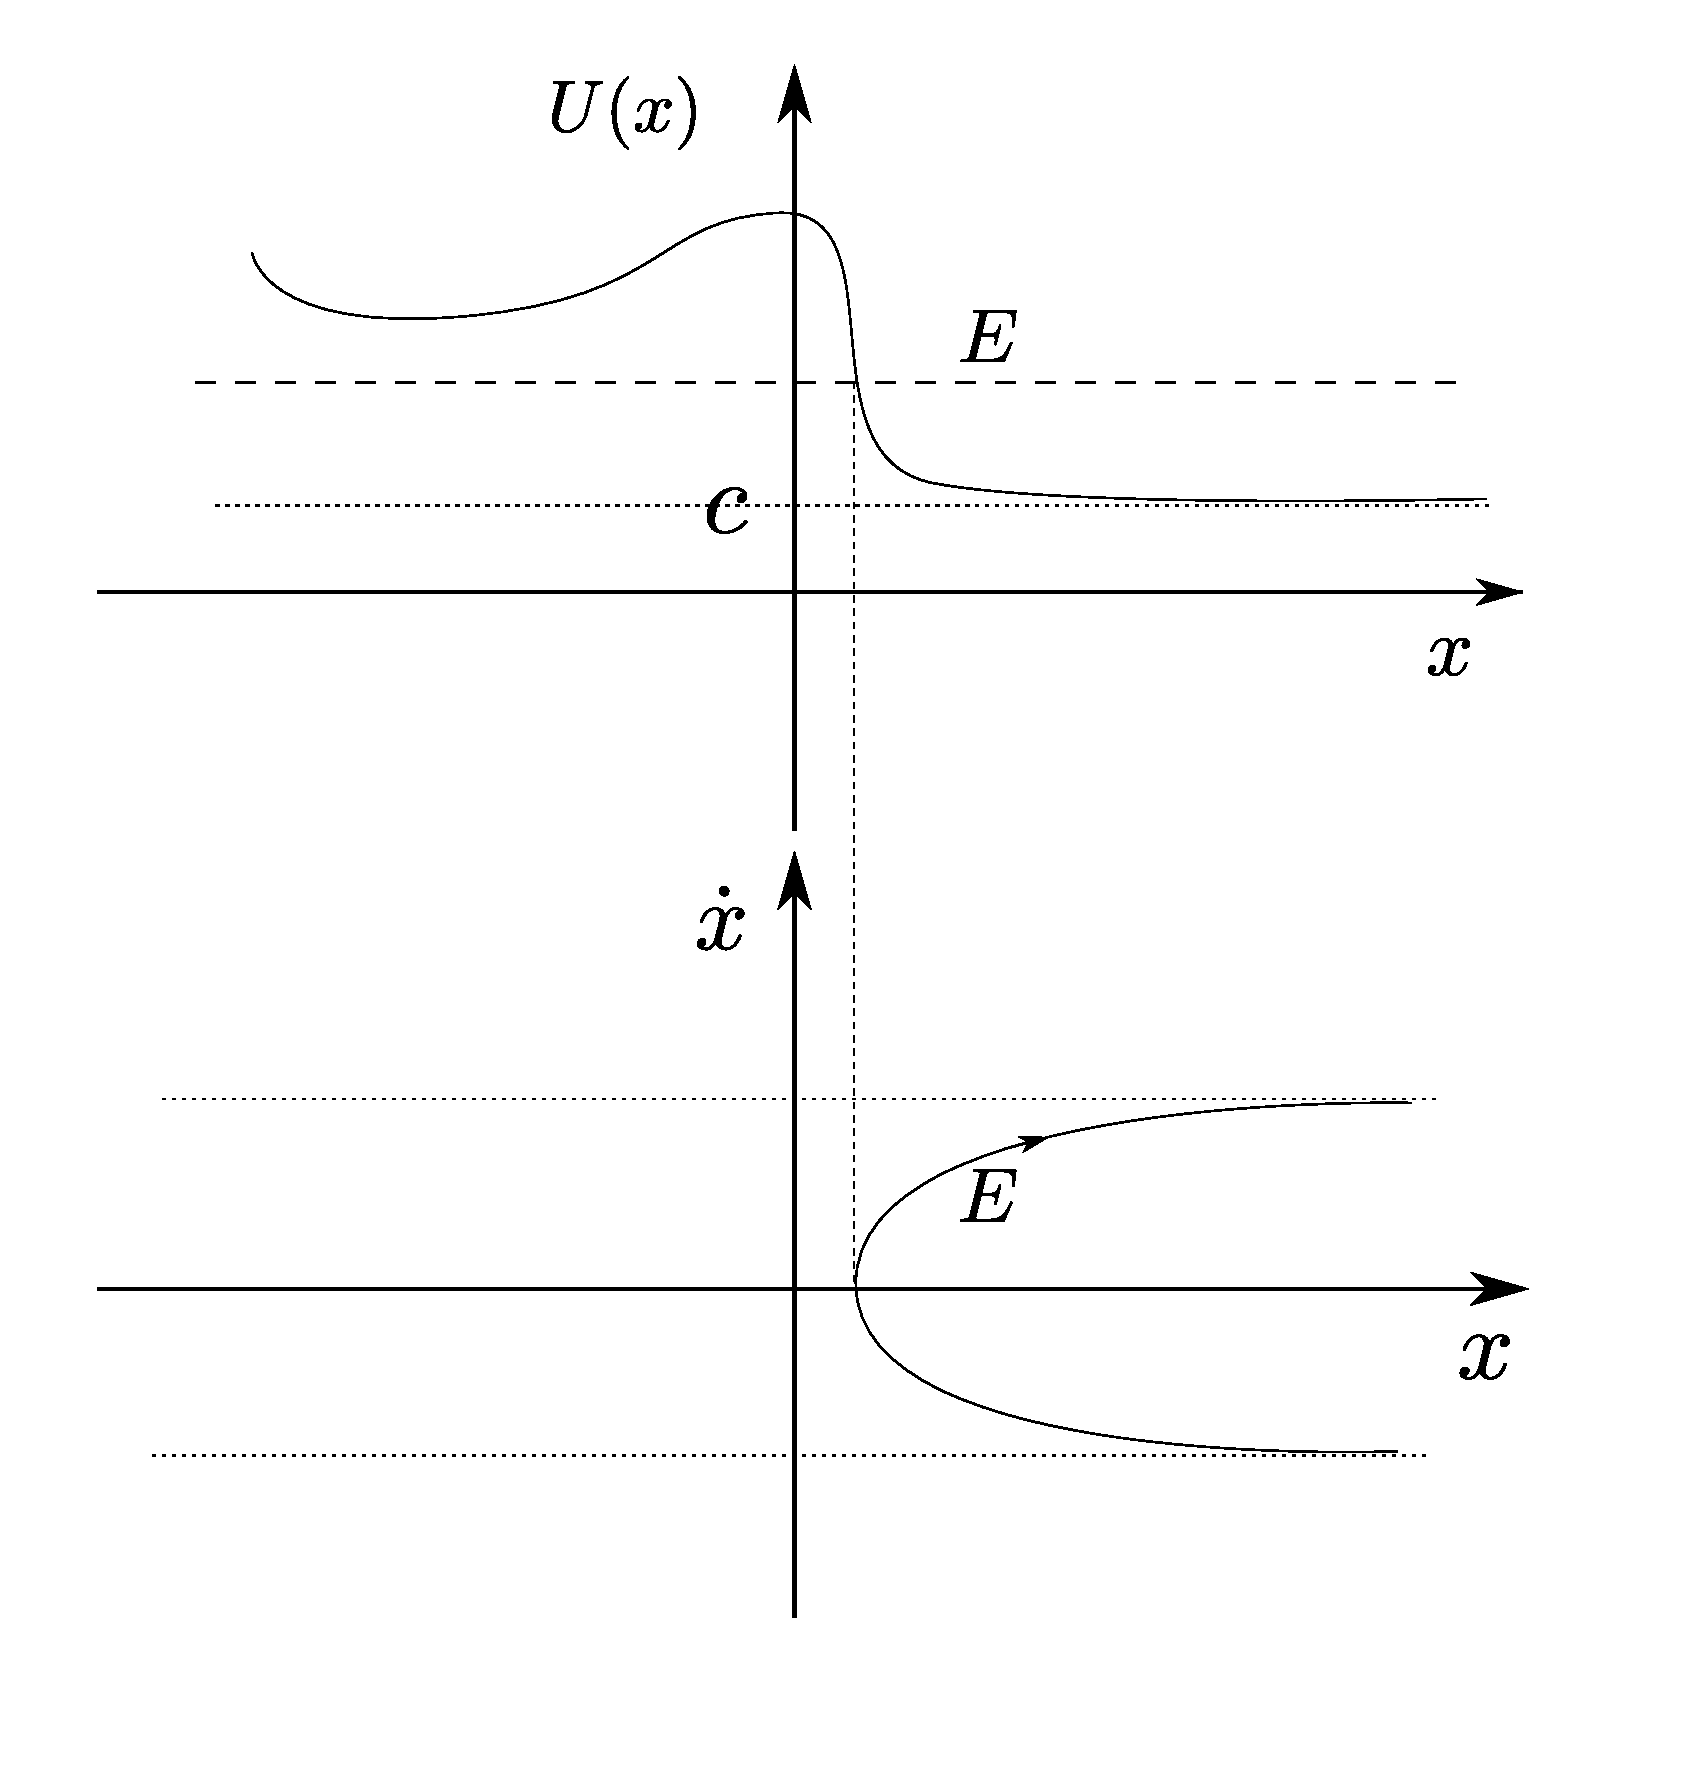
\includegraphics[width=0.75\textwidth]{images/inversion}
\end{figure}
Sostanzialmente nel ritratto di fase per energie sufficientemente vicine all'asintoto, cioè in modo che la parte di $U(x)$ che sta sotto l'energia scelta sia una funzione monotona. In particolare si hanno delle curve simili a "parabole" con asse sull'asse delle ascisse che per $x \rightarrow \infty$ tendono alla seguente velocità:
\begin{gather}
  \frac{mv^2}{2}=E-U(x)  \\\longrightarrow v= \pm \sqrt{\frac{2}{m} (E-U(x))} \\ \xrightarrow{x \rightarrow + \infty} v = \pm \sqrt{ \frac{2}{m}(E-c)}
\end{gather}
\end{appendic}



\begin{appendic}[Fuga all'infinito]

\begin{figure}[H]
    \centering
    \includegraphics[width=0.5\textwidth]{images/fuga}
\end{figure}


L'obbiettivo è trovare il tempo per raggiungere il punto $x=\pm \infty$. Ci si aspetta che questo sia possibile solo se $U(x)$ tende a $\mp \infty$ per $x\rightarrow \pm \infty$ (è come se esistesse un minimo di energia in questi punti).
Utilizzando di nuovo la conservazione dell'energia che di fatto caratterizza tutto il moto si ha:
	
\begin{equation}
  \frac{mv^2}{2}=E-U(x) \ \ \ (v = \dot x)
\end{equation}

	
\begin{equation}
  \dot x = \sqrt{\frac{2}{m}(E-U(x))}
\end{equation}

	separando le variabili e integrando tra $\xi$ e $+\infty$ (e prendendo $\xi$ abbastanza grande in modulo, altrimenti la particella potrebbe "incastrarsi" in dei minimi locali):
	
\begin{equation}
  	T(\xi)= \int _\xi ^{+\infty} \frac{dx}{\sqrt{\frac{2}{m}(E-U(x))}}
\end{equation}

	Supponendo che $U(x) \neq 0$ nell'intervallo considerato\footnote{non si perde di generalità, dopotutto basta traslare $U(x)$ senza avere grandi differenze nello studio del moto}, quindi l'unico problema sta nel fatto che si sta integrando su un intervallo infinito, ma supponendo che $U(x) \sim -x^\alpha$ per $x \longrightarrow +\infty$, $\alpha >0$ allora si ha che $\int_x ^\infty \frac{dx}{x^{\alpha / 2}}$ converge, cioè $T(\xi) < + \infty$, se e solo se $\alpha >2$. Ovviamente analogamente al caso di $\dot x=f(x)$ nella soluzione $x(t)$ nel piano $(t,x)$ la limitatezza di $T$ è rappresentata da un asintoto verticale in $t=T$ (detto anche tempo di blow-up), dopo tale istante la soluzione $x(t)$ cessa di esistere.
\end{appendic} 

\begin{appendic}[Buca infinita di potenziale]
    Si vuole studiare il moto di una particella costretta a muoversi nell'intervallo $[-l,l]$, quindi nei punti in cui si trova nell'intervallo in questione la particella si muove senza freni/accelerazioni (quindi forza nulla $\rightarrow \ U(x)=\text{cost}$), invece quando raggiunge i punti $\pm l$, incontra una barriera di potenziale che rimanda indietro. Non è semplice considerare un potenziale di questo tipo con punti angolosi, quindi si può pensare di considerare una successione $U_n$ che converge al potenziale $U_\infty$: 
	
\begin{equation}
  	m \ddot x = - U_n ' (x)
\end{equation}

\begin{equation}
  	U_n (x) = \epsilon \left( \frac{x}{l} \right)^{2n} \ \ \ n = 1, 2, ...
\end{equation}
\begin{osservazione}
	per $n=1$, $U_1 = \frac{\epsilon}{l^2} x^2 = \frac{k}{2}x^2$ \\
	E la funzione limite è:
\begin{equation}
  	\lim_{n \rightarrow + \infty} U_n (x) = \begin{cases}
		0, \ \ \ \ \ |x|<l \\
		\epsilon, \ \ \ \ \ |x| = l \\
		+ \infty , \ |x| >l
	\end{cases}
\end{equation}

\end{osservazione}

\begin{figure}[H]
    \centering
  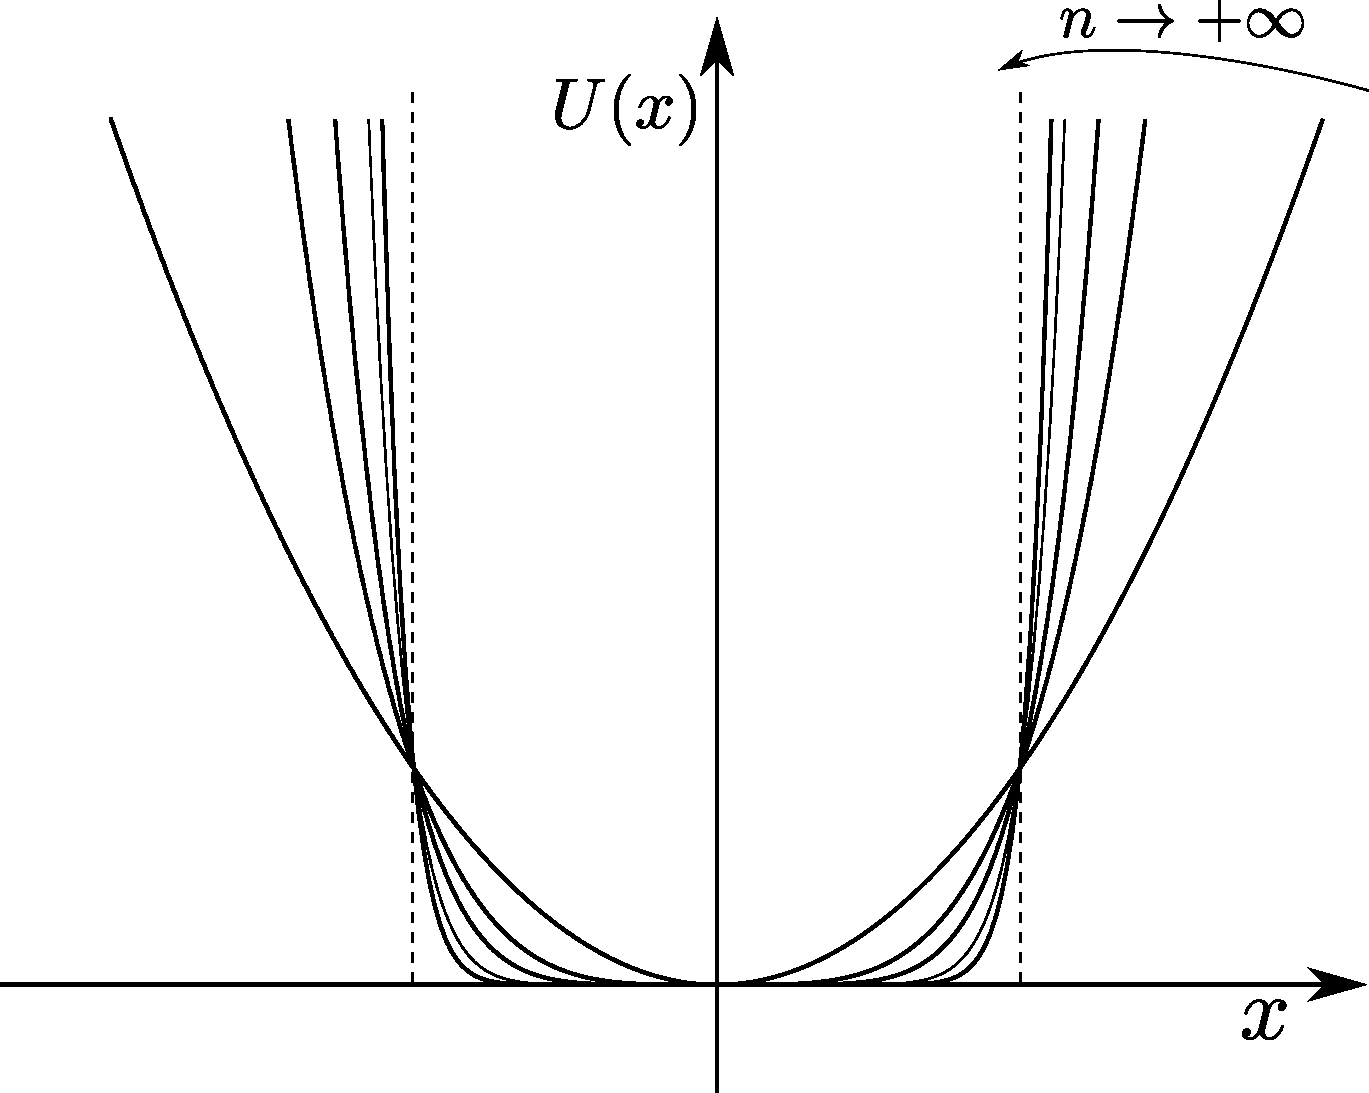
\includegraphics[width=0.6\textwidth]{images/boh}
\end{figure}

\noindent 
	\textbf{Diagramma di fase}\\
    Per $n$ fissato, aumentando $E$ la velocità nel punto di equilibrio aumenta sempre di più.
	Invece fissato E, aumentando solo n, i punti di inversione $x_\pm$ si avvicinano sempre di più a $x=\pm l$, invece il punto più alto della curva chiusa che collega tali punti di inversione, siccome l'energia è fissata, è sempre lo stesso, cosicché la curva chiusa tende a un rettangolo, quindi la velocità resta tende a rimanere costante nell'intervallo e la pallina resta intrappolata in un intervallo sempre più vicino a quello voluto. Infatti più rigorosamente abbiamo che i punti di inversione di trovano risolvendo $x_\pm : \ U_n(x) = E$.
\begin{equation}
  	\epsilon \left(\frac{x}{l}\right)^{2n} = E
\end{equation}
\begin{equation}
  	\rightarrow x_\pm = \pm l \left(\frac{E}{\epsilon}\right)^{\frac{1}{2n}}
\end{equation}
	che fissata una certa $E$:
\begin{equation}
  	\lim _{n \rightarrow \infty} x_{\pm} = \pm l
\end{equation}

\begin{figure}[H]
    \centering
  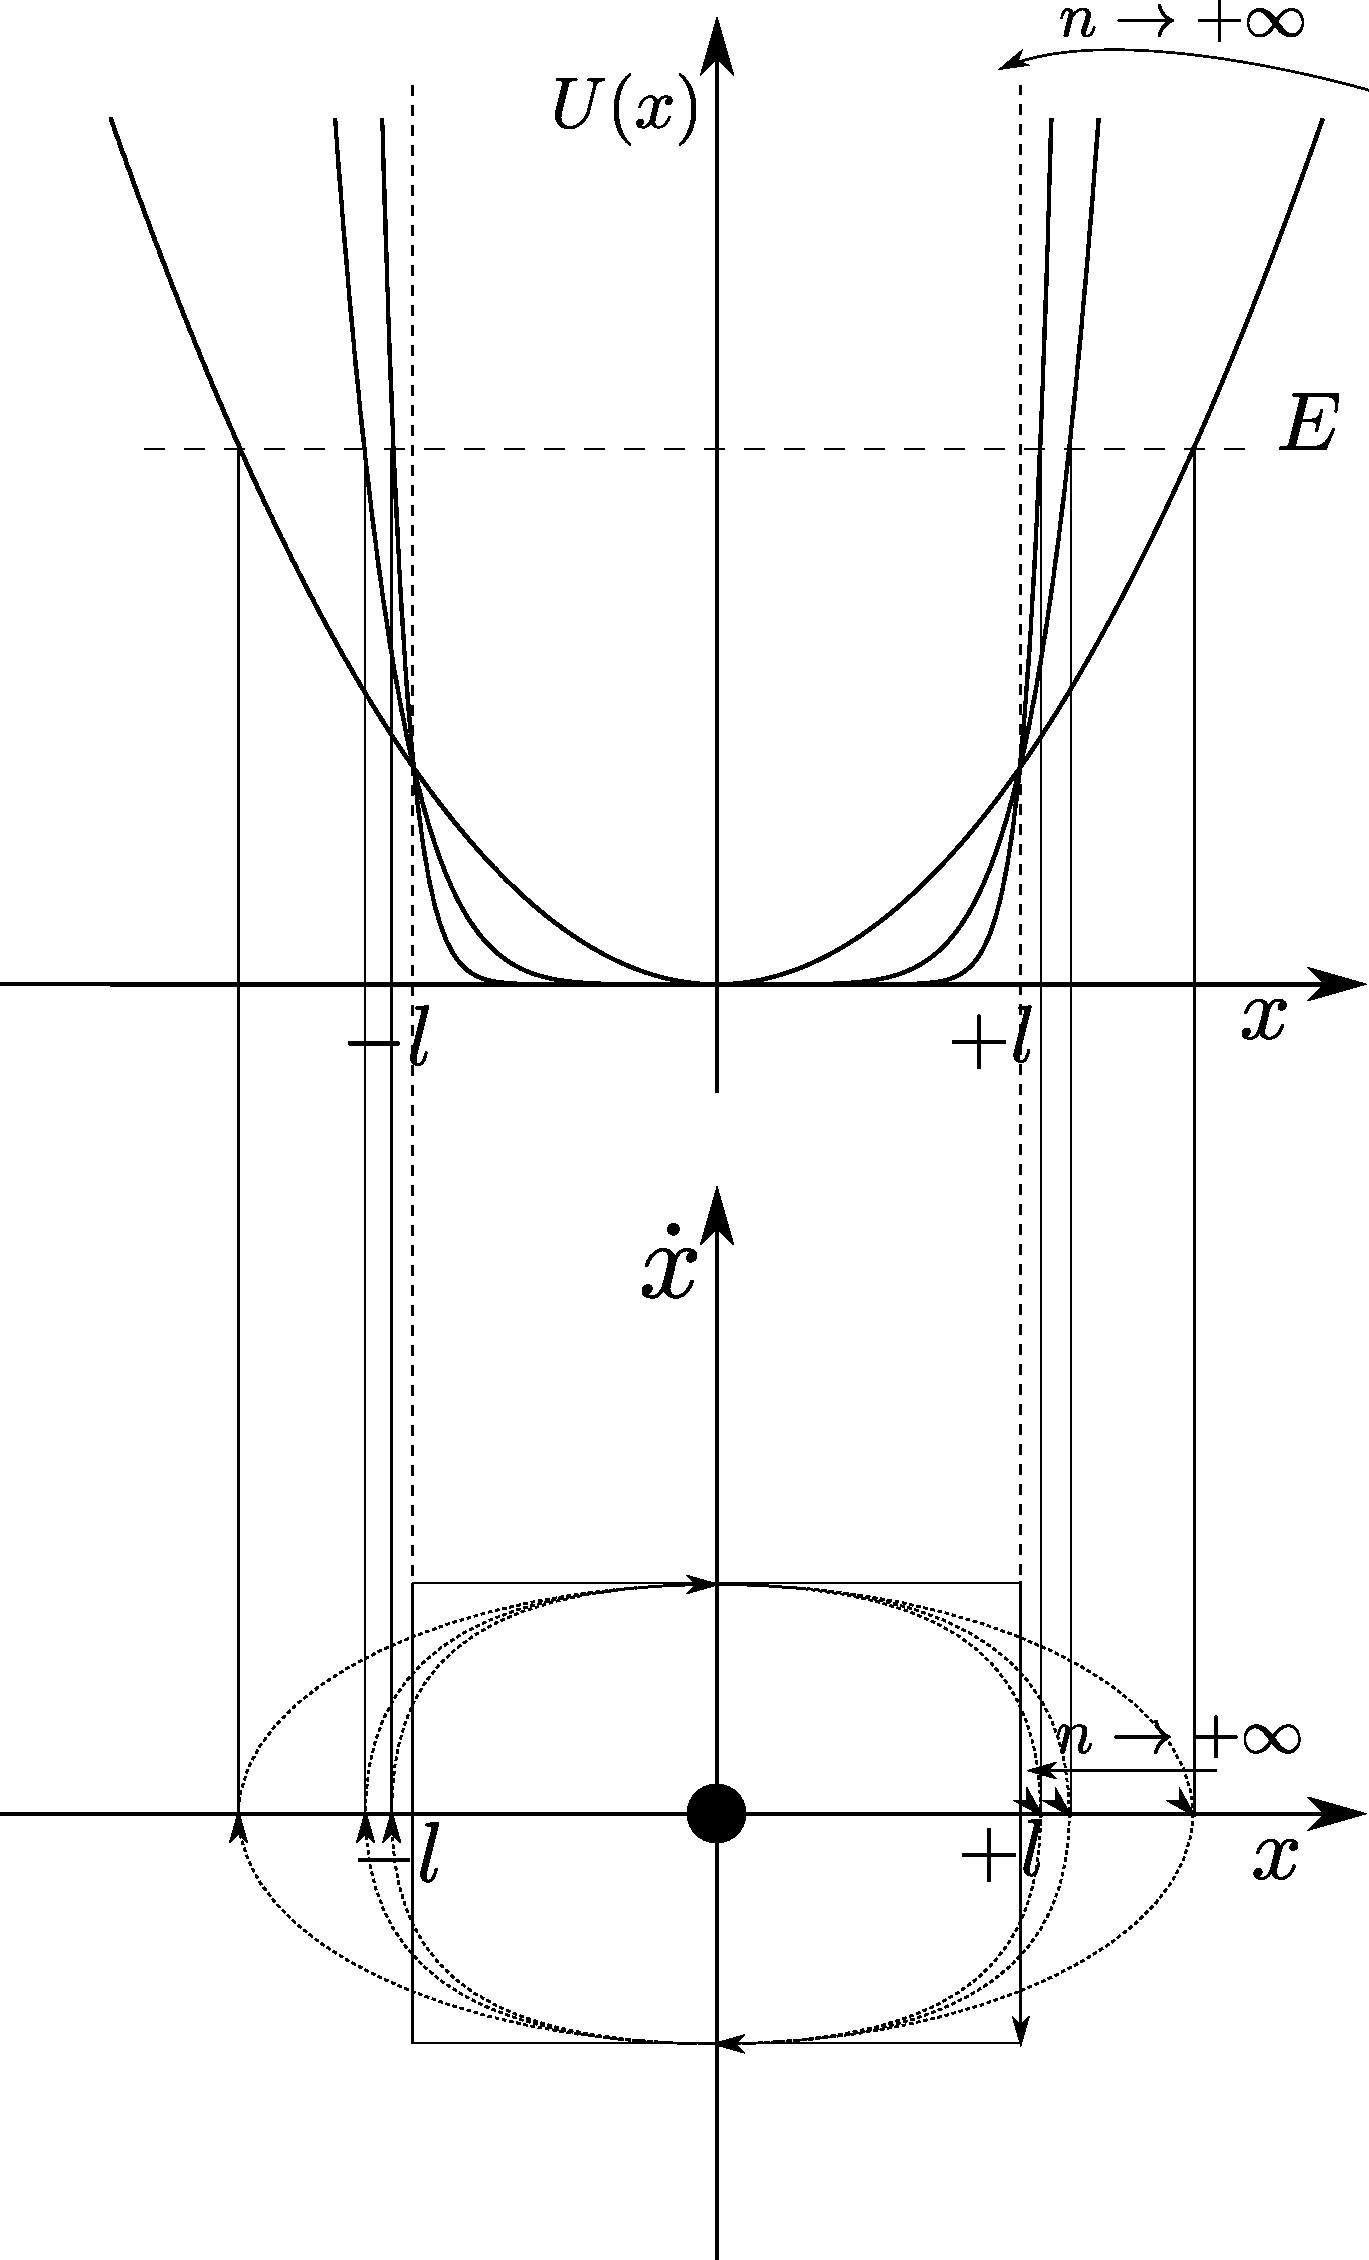
\includegraphics[width=0.5\textwidth]{images/pallina}
\end{figure}

	In modo analogo il periodo del moto si trova fissando una certa $E$:
\begin{equation}
  	T_n(E)= 2 \int_{x_-} ^ {x_+} \frac{dx}{\underbrace{\sqrt{\frac{2}{m}(E-U_n(x))}}_{\sqrt{v_+}}}
\end{equation}

\begin{equation}
  	=4 \int_0 ^{x_+} \frac{dx}{\sqrt{\frac{2}{m}(E-U_n(x)}} =
\end{equation}
\begin{equation}
  {x=x_+ \xi}
\end{equation}

\begin{equation}
  	=4 \int_0 ^1 \frac{x_+ d\xi}{\sqrt{\frac{2}{m}(E-E \xi ^{2n})}}
\end{equation}

\newpage
\begin{osservazioni}
	\item $U_n(x_+ \xi) =E \xi^{2n}$

	\begin{gather}
  T_n (E) = \frac{4 x_+}{\sqrt{\frac{2}{m}E}} \int_0 ^1 \frac{d \xi}{\sqrt{1- \xi ^{2n}}}\\
	= 2l \sqrt{2m}  \left( \frac{E}{\epsilon} \right)^{\frac{1}{2n}}E^{- \frac{1}{2}} \int_0 ^1 \frac{d\xi}{\sqrt{1-\xi^{2n}}}
\end{gather}

\item $1-\xi ^{2n}$ ammette la decomposizione

 $\underbrace{(1-\xi^2)}_{(1-\xi)(1+\xi)}(1+\xi^2+\xi^4+... + \xi^{2n-2})$. 

Quindi quando il potenziale è $U_\infty$:

\begin{equation}
  	\lim_{n\rightarrow \infty} T_n (E) = 2l \sqrt{2m} \left( {E} \right)^{- \frac{1}{2}}
\end{equation}
\end{osservazioni}

\noindent 
Per $n \rightarrow \infty$ vale che $\frac{mv^2}{2} = E \ \ ( -l<x<l)$

	$$
	v_\pm = \pm \sqrt{\frac{2}{m}E}
	$$

	$$
	T_ \infty (E) = 2 \frac{2l}{v^+}= 2l \sqrt{2m} E^{-\frac{1}{2}}
	$$
    che è lo stesso risultato trovato prima.
    Per trovare il periodo si può ricorrere al calcolo dell'area nello spazio delle fasi. Si calcola quindi l'area del diagramma di fase $A_\infty (E)$ nel piano $(x,p)$. Visto che è un rettangolo si può usare la formula $A= \text{base} \cdot \text{altezza}$:


\begin{gather}
	A_\infty (E) = 2l \ 2m v_+=\\
	= 4 lm \sqrt{\frac{2}{m}E} = 4 \sqrt{2m} \ l \sqrt{E}\\
	\Rightarrow \frac{dA_\infty}{dE} = T_\infty
\end{gather}
Esattamente come già trovato prima.\\
	Supponendo adesso che l'area possa assumere valori del tipo $A_\infty = sh$, con $h$ costante di Planck e $s$ numero naturale. Ma dall'altra parte l'area si scrive ancora come l'area di un rettangolo (esattamente come prima):
\begin{equation}
  	\rightarrow sh = 4 \sqrt{2m} \ l \ \sqrt{E}
\end{equation}
	isolando
\begin{equation}
  	E_s = \frac{s^2 h ^2}{32 m l^2}
\end{equation}
Si ha la quantizzazione dell'energia. Queste sono le energie permesse per particelle quantistiche nella scatola monodimensionale. \bigskip 

\noindent 
\textbf{Invarianza di scala del problema}
\\
Notando che $U_n(x)$ è omogenea di grado $2n: \ U_n (\lambda x) = \lambda ^{2n} U_n (x)$
\\$
\Rightarrow f_n(x) = - U_x'(x)
$ è omogenea di grado $2n-1$. Questo è un fatto essenziale perché ciò significa che esistono dei riscalamenti per le $x$ e $t$ particolari tale per cui il problema resta appunto invariante. Intanto partendo dall'eq. di newton si ha:
\begin{equation}
  m \frac{d^2}{dt^2} x = f_n(x)
\end{equation}

Ora riscalando $x$ con $\lambda x'$ e riscalo $t$ con $\lambda^\alpha t'$. Sostituendo si ha:

\begin{equation}
  m \frac{\lambda}{\lambda^{2\alpha}}\frac{d^2}{dt'^2} x' = f_n (\lambda x') = \lambda ^{2n-1} f_n(x')
\end{equation}
È importante notare che proprio perché $f_n$ è omogenea che si può cercare di far sparire $\lambda$ (altrimenti questa rimarrebbe intrappolata dentro l'argomento della funzione), cioè di rendere l'equazione, e quindi il moto, non dipendente dal particolare valore di $\lambda$. Infatti isolando i $\lambda$:
\begin{equation}
  m \frac{d^2}{dt'^2}x' = \lambda^{2n-2+2 \alpha} f_n (x')
\end{equation}
Questa equazione è indipendente da $\lambda$ $\iff 2n-2 + 2 \alpha =0$. Quindi risulta $\alpha = 1-n$. E così si è trovato il riscalamento corretto. Però ora interessa anche sapere come cambia l'energia $E$ sotto questo riscalmento. Il calcolo porta a:

\begin{gather}
  E= \frac{m}{2} \left( \frac{d}{dt}x \right)^2 + U_n (x)\\ \text{riscalando} \Rightarrow \frac{\lambda^2}{\lambda^{2(1-n)}} \frac{m}{2} \left(  \frac{dx'}{dt'}\right) ^2 + \lambda ^{2n} U_n (x')=\\
  \lambda^{2n} \left( \frac{m}{2} \left( \frac{dx'}{dt'} \right)^2 + U_n (x') \right) = \lambda^{2n} 
\end{gather}

Quindi il gruppo di scala è $\begin{cases}
	x= \lambda x' \\
	t= \lambda ^{1-n} t' \\
	E= \lambda ^{2n} 
\end{cases}$

Quindi riassumendo si è visto che $U_n$ è omogenea, questo implica che riscalando $x$ esiste uno riscalamento per $t$ tale che l'equazione di newton nuova in $x'$ e $t'$ non risente del particolare valore di $\lambda$. Questo cosa significa? Significa che se si misurano certe quantità in questo nuovo sistema di coordinate non serve accorgersi del particolare riscalamento che si è addottato. Per esempio se si misurano delle lunghezze e ne se ne fa il rapporto con una certa potenza dell'energia associata si deve ottenere la stessa costante che si è ottenuto con $x$ e $t$. Infatti prendendo la prima equazione e l'ultima (che è stata ottenuta perchè tutte le quantità ricavate precedentemente sono espresse in termini dell'energia), si deve elevare la seconda alla $\frac{1}{2n}$ per avere l'uguaglianza di si è parlato appena sopra:
\begin{equation}
   \frac{x}{E^{1/2n}} = \frac{\cancel{\lambda} x'}{\cancel{\lambda}^{1/2n}} = \frac{x'}{è^{ \frac{1}{2n}}}= \text{costante indipendente da $\lambda$} 
\end{equation}
Questo consente di dire che una qualsiasi lunghezza misurata sarà proporzionale all'energia associata:
\begin{gather}
	\Rightarrow x_+ - x_- \propto E^{1/2n}\\
	\Rightarrow x_\pm \propto E^{1/2n}
\end{gather}
Una cosa analoga avviene per i tempi: fissando una certa energia, misurando qualche tempo e se si calcola il rapporto questo deve essere una costante indipendente da $\lambda$. Infatti:
\begin{equation}
  \frac{t}{E^{\frac{1-n}{2n}}}=\frac{\cancel{\lambda ^{1-n}}t'}{\cancel{\lambda^{1-n}} E^{,\frac{1-n}{2n}}}
= \frac{t'}{E^{,\frac{1-n}{2n}}}
\end{equation}
E quindi un qualsiasi tempo è proporzionale a $E$, in particolare il periodo:
\begin{equation}
  T(E) \propto E^{-\frac{1}{2}+\frac{1}{2n}}
\end{equation}

\bigskip
In questo ambito il metodo con cui si è ricavata la particolare forma della forza di gravità di Newton diventa chiaro: Keplero misurò dei tempi (periodi) e lunghezze associate (semiassi maggiori) e notò che il rapporto tra i due (con certe potenze) era una costante indipendente (per esempio) dall'asse maggiore, cioè le due quantità erano proporzionali (con certi esponenti), ma allora il problema gode di invarianza di scala (con certi esponenti del fattore di scala), e quindi l'eq. di Newton associata deve essere indipendente da $\lambda$. E qui il ragionamento va nel verso opposto: è possibile cercare gli esponenti giusti per avere l'invarianza di scala e da cui trovare le relazioni che sussistono tra le varie quantità associate.
\end{appendic}

\newpage

\begin{appendic}[Equazione logistica] 
 Considerando la seguente equazione:
\begin{equation}
  \dot x = k x (1- \frac{1}{p} x)
\end{equation} 
Dove $k$ è detto il tasso di riproduzione e $p$ la capacità di portata.L'equazione è chiamata anche equazione logistica.

Ridefinendo le due variabili $t$ e $x$ nel seguente modo:
\begin{gather}
	y= \frac{x}{p}\\
	\tau =kt
\end{gather}
l'equazione differenziale si riduce a:
\begin{equation}
  \Longrightarrow \frac{dy}{d \tau} = y(1-y)
\end{equation}
Cioè tutti i sistemi logistici visti ad una appropriata scala di tempi e di popolazione appaiono identici.\\
Graficando si ottiene:

\begin{figure}[H]
    \centering
  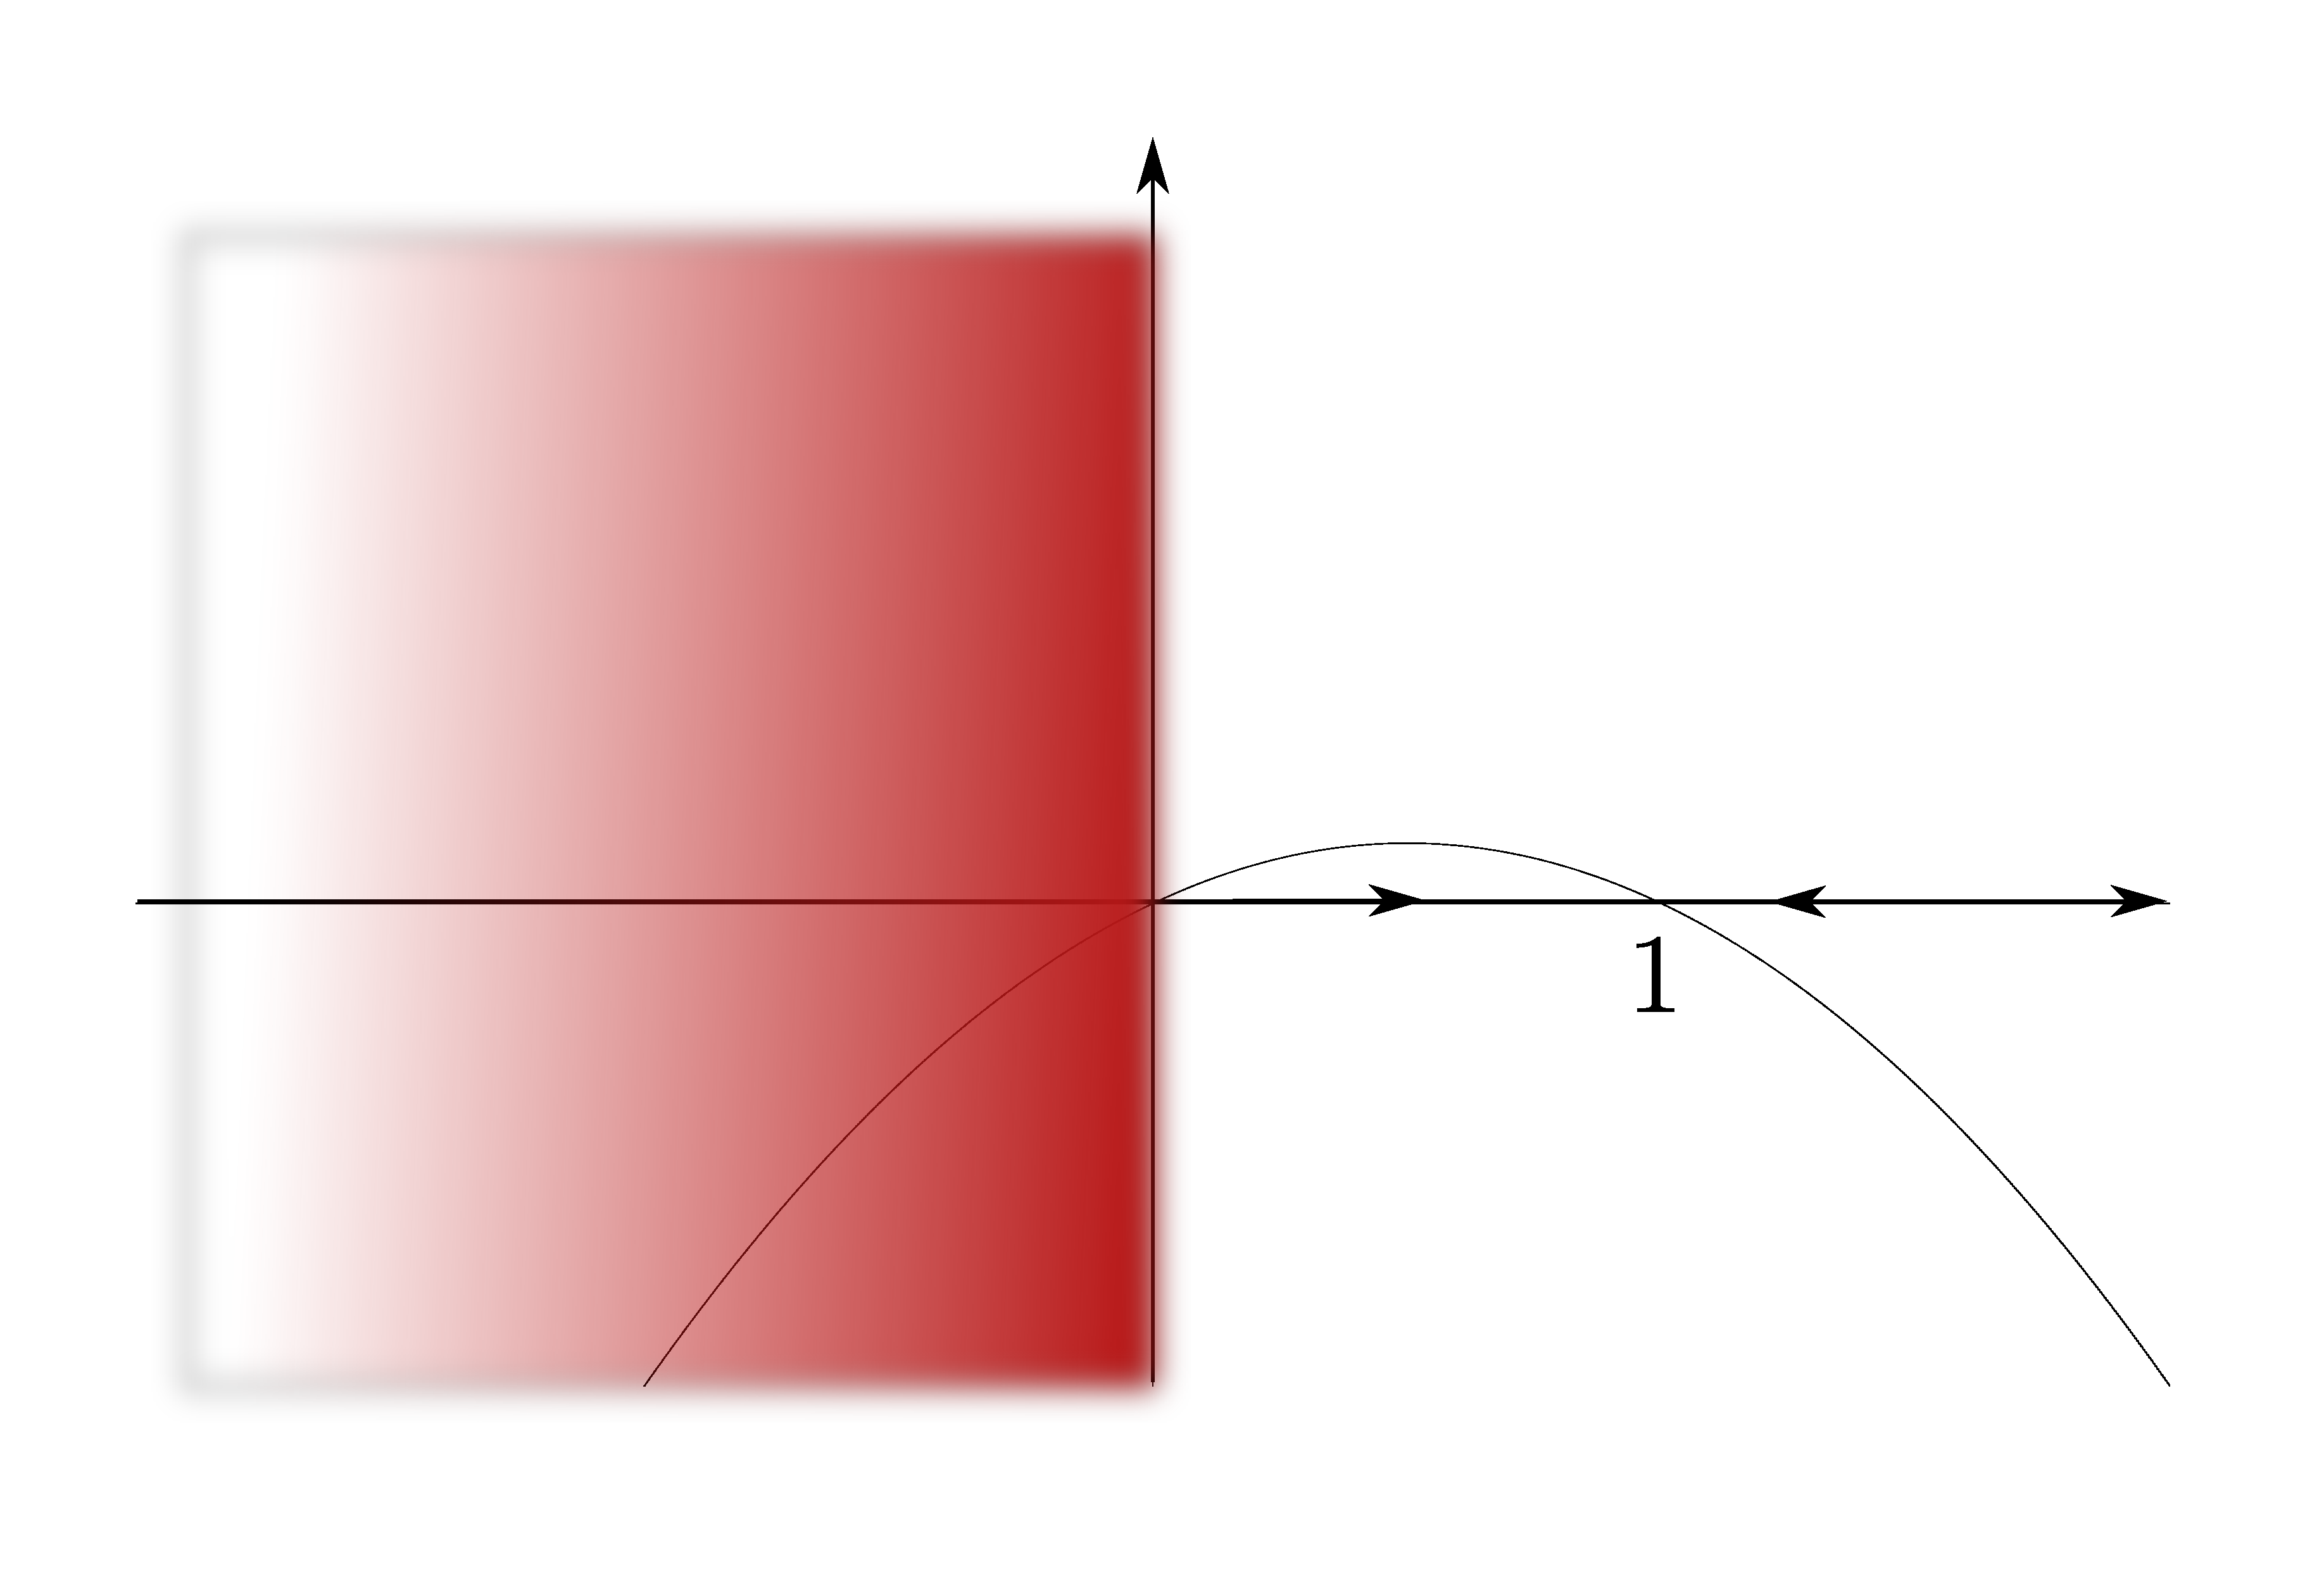
\includegraphics[width=0.5\textwidth]{images/portata.pdf}
\end{figure}

Da cui si vede che lo zero (0) è instabile mentre lo zero (1) è equilibrio stabile, la popolazione tende sempre alla portata. L'equazione è un primo tentativo di modellizzare l'andamento delle popolazione dove esiste una portata del sistema ben precisa fissata a priori e può essere decisa in base alle risorse presenti. Se la popolazione è minore della portata allora questa cresce perché ci sono abbastanza risorse per tutti, altrimenti decresce in modo analogo. Vicino alla portata la crescita/decrescita della popolazione è esponenziale, è sufficiente risolvere l'equazione differenziale per vederlo.
\end{appendic}

\begin{appendic}
[Modello SIR (propagazione di malattie virali)]
Sia $N(t)$: numero totale di casi al tempo $t$; $(N(t) = I(t) + R(t))$, dove $I(t)$ sono gli infetti e $R(t)$ sono i guariti o i morti\footnote{In alcuni modelli epidemiologici si studiano separatamente le popolazioni guarite e quelle decedute, ma qui si può fare questa semplificazione perché si considera che si può prendere la malattia una sola volta.}.
Chiamando $P$ la popolazione totale è possibile definire la percentuale di casi sul totale come $n(t) := \frac{N(t)}{P}$. Questa quantità è soluzione della seguente equazione differenziale\footnote{Attenzione, nel mondo reale $n(t)$ è una funzione a valori discreti, quindi in teoria l'equazione sarebbe un'equazione a differenze finite, ma le due danno risultati praticamente uguali nel caso in cui $P$ sia molto grande.}
\begin{equation}
  \dot n = a(1-n)\left(n+ \frac{1}{R_0} \ln (1-n) \right):= f(n)
 \hspace{1cm} con \ n \geqslant 0 
\end{equation}
dove le varie costanti hanno il seguente significato:
\begin{equation}
  \begin{cases}
	a: tasso \ di \ contagio \\
	b: tasso \ di \ "rimozione"\\
	R_0 : \frac{a}{b} \ (numero \ di \ riproduzione \ iniziale )\\
\end{cases}
\end{equation}
Se $R_0>1$ la pandemia si espande, invece se $R_0<1$ si spegne.

L'ipotesi è che la popolazione dei suscettibili $S(0) \approx P$. Un'altra ipotesi è l'immunità, ovvero chi si ammala non può ricontrarre la malattia (infatti al totale dei casi si è sommato oltre agli infetti anche i ricoverati e "non si torna indietro").

Non si riesce dare una soluzione esatta esplicita (si può sempre risolvere al computer), ma possiamo comunque farne uno studio qualitativo. Si vuole trovare in particolare gli zeri del campo vettoriale (membro di sinistra) e per fare ciò c'è bisogno dello studio di funzione di tale equazione. Intanto si nota che c'è uno zero banale in $n=0$, un equilibrio instabile/repulsivo infatti:
\ se $n<<1$ allora $\ln(1-n) \approx -n$ e si ha

\begin{equation}
  \dot n \approx a(1-n)n \left(1-\frac{1}{R_0} \right)=(a-b)(1-n)n
\end{equation}

E diventa un modello con comportamento logistico. Si nota che inizialmente i casi crescono esponenzialmente, infatti $f(n)\approx (a-b)n$. In particolare la funzione $f(n)$ è positiva per $n\rightarrow 0^+$ confermando che lo zero in $n=0$ è repulsivo (da destra).

C'è anche uno 0 semplice per $n \rightarrow 1$, infatti nonostante la funzione non sia definita per $n=1$, ne esiste comunque il limite, cioè è una discontinuità eliminabile. Invece per la natura dell'equilibrio andiamo a vedere la pendenza nel punto $n=1$:
\begin{equation} \notag
  f'(n) = a \left[-1 \left(n + \frac{1}{R_0} \ln(1-n)\right) + (1-n)\left(1- \frac{1}{R_0} \frac{1}{1-n} \right) \right]
\end{equation}

\begin{equation}
  =a \left[1-2n - \frac{1}{R_0} \ln(1-n) - \frac{1}{R_0} \right]
\end{equation}
\begin{equation}
  \lim_{x \rightarrow 1^-} f'(n) = + \infty
\end{equation}
Quindi la pendenza di $f(n)$ in $n=1$ è positiva, cioè la $f(n)$ è negativa per $n\rightarrow 1^-$, quindi $n=1$ è un equilibrio repulsivo.\\
Per $n\rightarrow 0^+$ la $f(n)$ è positiva, invece per $n \rightarrow 1^-$ negativa, quindi esiste uno zero intermedio $\tilde n$, e questo sarà anche il nostro unico equilibrio stabile/attrattivo.

\begin{figure}[H]
    \centering
  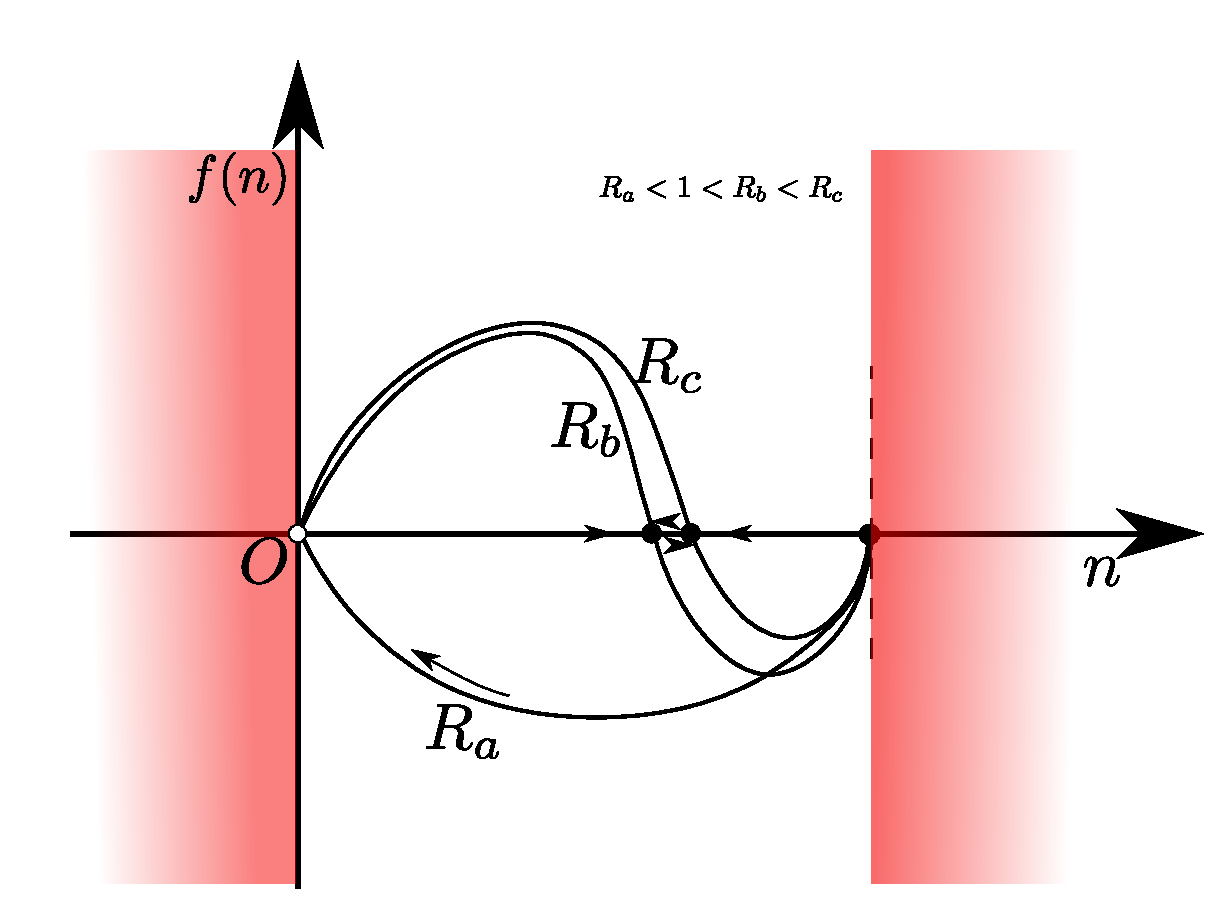
\includegraphics[width=0.5\textwidth]{images/sir.pdf}
\end{figure}

\newpage \noindent 
\textbf{Metodo delle tangenti di Newton-Raphson}\\
 
\begin{figure}[H]
    \centering
  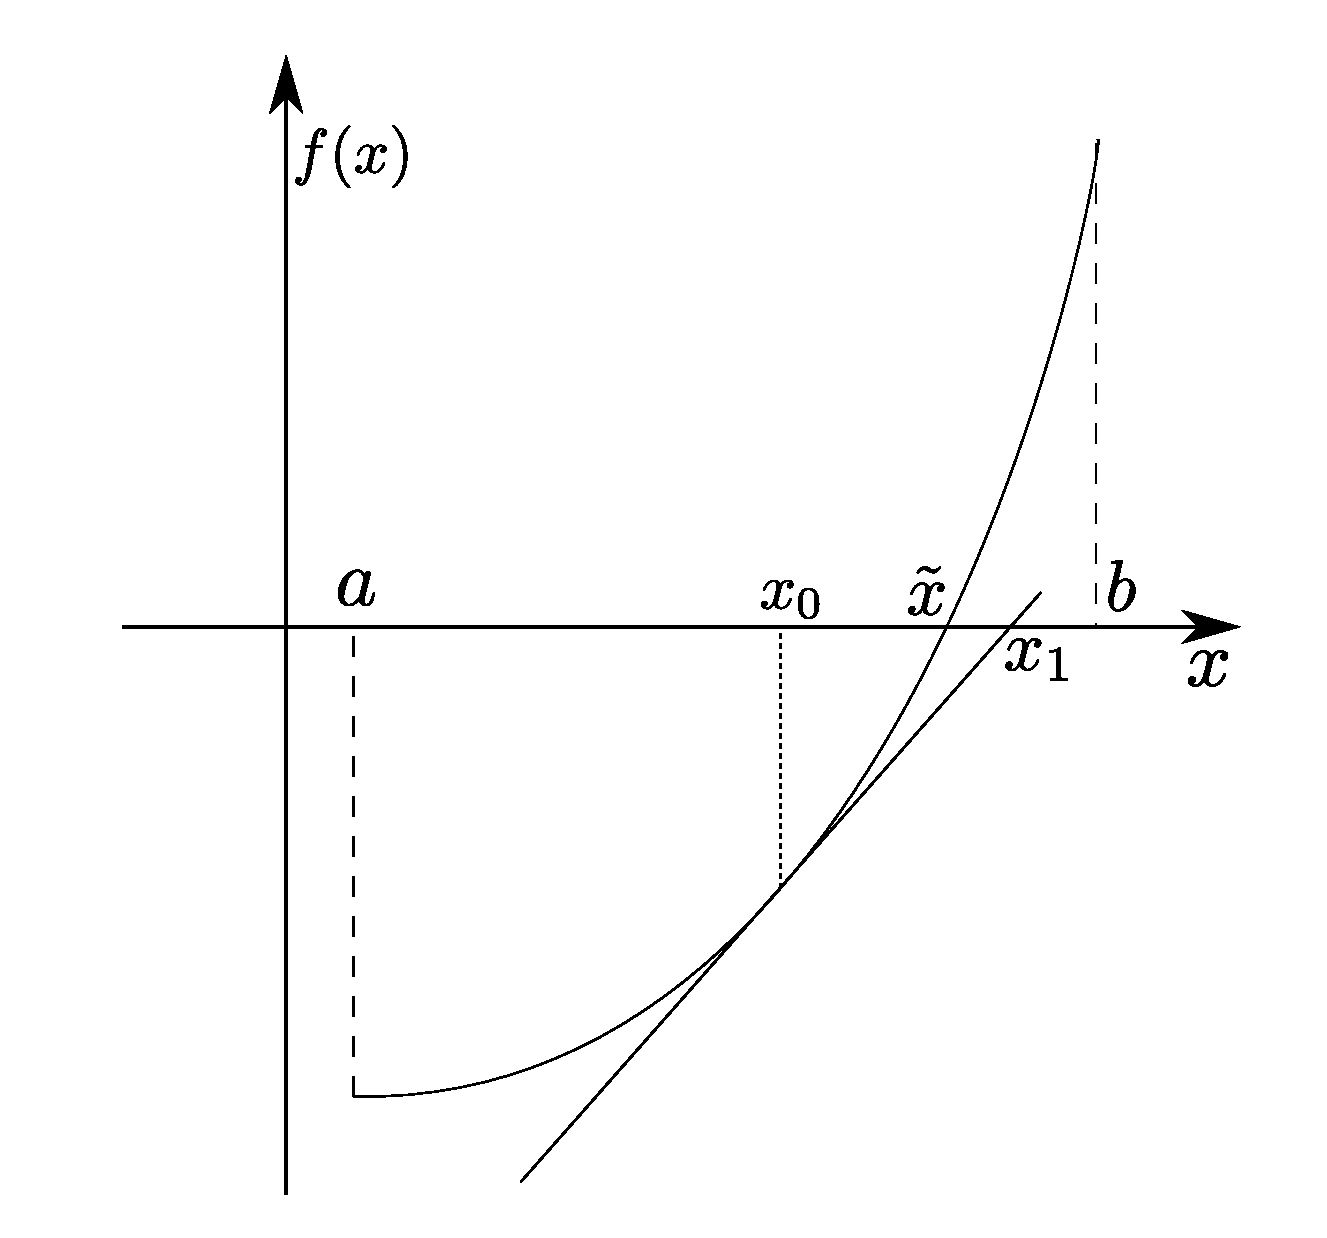
\includegraphics[width=0.5\textwidth]{images/metodotangenti.pdf}
\end{figure}   	
Per calcolare il secondo zero $\tilde n$ si può utilizzare il metodo delle tangenti di Newton-Raphson. Questo metodo si applica in piccoli intervalli,

\begin{equation}
  x \mapsto f(x), \ x \in [a, b]
\end{equation}

Le ipotesi per applicare questo metodo sono:
\begin{itemize}
	\item $
f'(x) \neq 0, \ \forall x \in [a,b]
$
\item $
f(a)f(b)<0
$
\end{itemize}
Allora esiste (unico) $\tilde x \in ]a,b[$ tale che $f(\tilde x)=0$.\\
Per partire si sceglie un $x_0$ nell'intervallo e si calcola la retta tangente al grafico di f in $x_0$

\begin{equation}
  y=f(x_0) + f'(x_0)(x-x_0)
\end{equation}
La retta ha uno zero in $x_1$ tale che $f(x_0) + f'(x_0)(x_1-x_0)=0$
\begin{equation}
  \rightarrow x_1=x_0 - \frac{f(x_0)}{f'(x_0)}
\end{equation}
Iterando questi passaggi si ottiene una successione definita per ricorrenza:
\begin{equation}
  x_{n+1}= x_n - \frac{f(x_n)}{f'(x_n)}
\end{equation}
Questa successione ha soluzione $x_n = \tilde x, \ \forall n \in \mathbb{N}$. Si dimostra che $\forall x_0 \in [a,b]$ $\lim_{n\rightarrow \infty} x_n = \tilde x$ (sotto le ipotesi fatte). Il fatto interessante è che l'algoritmo converge molto velocemente e spesso basta una sola iterazione. Ciò sarà vero anche in questo caso.


Tornando al modello SIR, prima di studiare la funzione con il metodo di Newton-Raphson, si definisce $u := 1-n$ perché semplifica i calcoli e sopratutto perché si è interessati a sapere quanto lontano ci si ferma rispetto al contagiare tutti. Si ottiene:
\begin{equation}
  g(u) = 1-u + \frac{1}{R_0} \ln(u)=0
\end{equation}
Intanto è facile vedere il valore della funzione agli estremi dell'intervallo in cui è definita che risultano essere ancora (0,1): \newline
$g(0^+)= - \infty$\\
$g(1)=0$\\
Quindi la funzione è negativa per $u=0^+$ e nulla per $u=1$, noi ci si aspetta che lì in mezzo esista un altro valore $\tilde u$ tale che $g(u)=0$, da cui si troverà $\tilde n =1-\tilde u$. Ma per applicare l'algoritmo bisogna mettersi in un intervallo in cui si è sicuri che la funzione cambi segno e non abbia punti stazionari. Ma provando a calcolare la derivata rispetto $u$ si ha:
$g'(u)=-1+ \frac{1}{R_0 u}>0$
infatti
\begin{equation}
  \frac{1}{R_0 u} > 1 \iff u < \frac{1}{R_0}
\end{equation}
Quindi la funzione $g(u)$ parte negativamente dal punto $u=0$ e cresce in modo monotono fino a $u=\frac{1}{R_0}$ cui corrisponde un valore positivo della $g(u)$. Si è nelle condizioni per applicare l'algoritmo di Newton-Raphson. La mappa dal metodo Newton-Raphson da iterare è:
\begin{equation}
  u_{n+1}= u_n - \frac{g(u_n)}{g'(u_n)}
\end{equation}
\begin{equation}
  = u_n - \frac{1- u_n + \frac{1}{R_0} \ln(u_n)}{-1 + \frac{1}{R_0 u_n}}
\end{equation}

Per $u_0$ potremmo prendere un qualsiasi $u<1/R_0$, ma prendendo la soluzione di $1 + \frac{1}{R_0} \ln(u)=0$ cioè $u_0=e^{-R_0}$ perché ciò ci permette di semplificare notevolmente l'espressione di $u_1$ (vedere il numeratore dell'equazione precedente). Inoltre è interessante notare che effettivamente $e^{-R_0}<\frac{1}{R_0}$. Quindi sostituendo $u_0$ in $u_n$ e calcolando $u_1$ abbiamo:

\begin{equation}
  u_1 = u_o - \frac{1- u_0 + \frac{1}{R_0} \ln (u_0)}{-1 + \frac{1}{R_0 u_0}}
\end{equation}

\begin{equation}
  = e^{-R_0}- \frac{1- e^{-R_0}-1}{-1 + \frac{1}{R_0} e^{R_0}}= e^{-R_0}+ \frac{e^{-R_0}}{\frac{1}{R_0} e^{R_0} -1}
\end{equation}
\begin{equation}
  u_1 = e^{-R_0} \left(1+ \frac{1}{\frac{1}{R_0} e^{R_0} -1} \right)
\end{equation}
Se $R_0=3$ si ottiene la frazione (secondo termine parentesi) $*=0.17$, se $R_0 = 5 \rightarrow 0.03$. Già per $R$ modesti l'equilibrio stabile è praticamente uguale a n=1 e ci si avvicina esponenzialmente con $R_0$.	
\end{appendic}





\newpage
\appendice{Altri esempi di potenziale}

\begin{appendic}[Oscillatore armonico non semplice]
\begin{equation}
  m \ddot x = - kx + \alpha x^3
\end{equation}

\begin{equation}
  U(x)= \frac{k}{2}x^2 - \frac{\alpha}{4}x^4
\end{equation}

Il caso $\alpha=0$ è stato già studiato molte volte, quindi $\alpha \neq 0$. Inoltre per $\alpha <0$ il potenziale non è molto diverso dal potenziale armonico semplice, quindi il diagramma di fase è praticamente identico (ma le curve di livello \textit{non} sono ellissi).
Quindi si studia il caso $\alpha >0$. Si disegna $U(x)$ tramite uno studio di funzione, e dopodichè quello che si è sempre fatto: si sceglie un energia vicino ad un minimo/massimo, si disegna la curva di livello relativa, si alza/abbassa l'energia, si disegna la curva di livello etc. Inoltre si nota che siccome $U(x)$ è pari, il ritratto di fase sarà simmetrico anche rispetto all'asse $v$.

\begin{figure}[H]
    \centering
    \includegraphics[width=0.5\textwidth]{images/casinoo}
\end{figure}

 Per $E=E_c$ (energia dei massimi locali) ci sono 8 moti possibili: due soluzioni di equilibrio, soluzioni degeneri in quattro asintoti e due soluzioni \textit{eterocline} (connettono due equilibri).

\begin{figure}[H]
    \centering
    \includegraphics[width=0.5\textwidth]{images/Ealta}
\end{figure}

 Aumentando ancora il livello di $E$ si ottengono 2 moti possibili. Le curve di livello relative sono aperte.
Per ultimo si può fare una classificazione veloce dei 3 equilibri (sostanzialmente vedere se sono zeri di $U(x)$ con $\frac{d^2 U}{dx^2}(x) \neq 0$):

\begin{equation}
  U(x) = 0 \longrightarrow \frac{kx^2}{2}= \alpha \frac{x^4}{4}
\end{equation}

Le cui soluzioni sono $x=0$ e $\tilde x _ \pm = \pm \sqrt{\frac{2k}{\alpha}}$.

\begin{equation}
  (x)=0 \longrightarrow kx -\alpha x^3 = 0
\end{equation}

Le cui soluzioni sono $x=0$ e $\tilde x _\pm = \pm \sqrt{\frac{k}{\alpha}}$
\begin{equation}
  U'(x) = k - 3 \alpha x^2 \Longrightarrow U'(\tilde x_\pm) = k- 3 \alpha \tilde x _ \pm ^ 2 = k - 3 \cancel{\alpha} \frac{k}{\cancel{\alpha}}= -2k <0
\end{equation}

E quindi gli zeri sono tutti non degeneri: $(0,0)$ centro; $(\tilde x_ \pm , 0) $ sono due punti iperbolici (o di sella).\\
\begin{osservazione}
	Siccome:
\begin{equation}
  	\frac{mv^2}{2} + \frac{k}{2} x^2 - \frac{\alpha}{4} x^4 =E
\end{equation}
	si ha:
\begin{equation}
  	\longrightarrow v_+(x)= + \sqrt{\frac{2}{m}(E- \frac{k}{2}x^2 + \frac{\alpha}{4}x^4)}
\end{equation}
	E quindi $v_+ \sim x^2, x \longrightarrow + \infty$ da cui acquisisce anche la concavità verso alto.
\end{osservazione}
\end{appendic}

\begin{appendic}[Oscillatore armonico traslato]
\begin{equation}
  \dot x = x^2 - \epsilon
\end{equation}
Caso: $\epsilon=0$
	\begin{figure}[H]
    \centering
  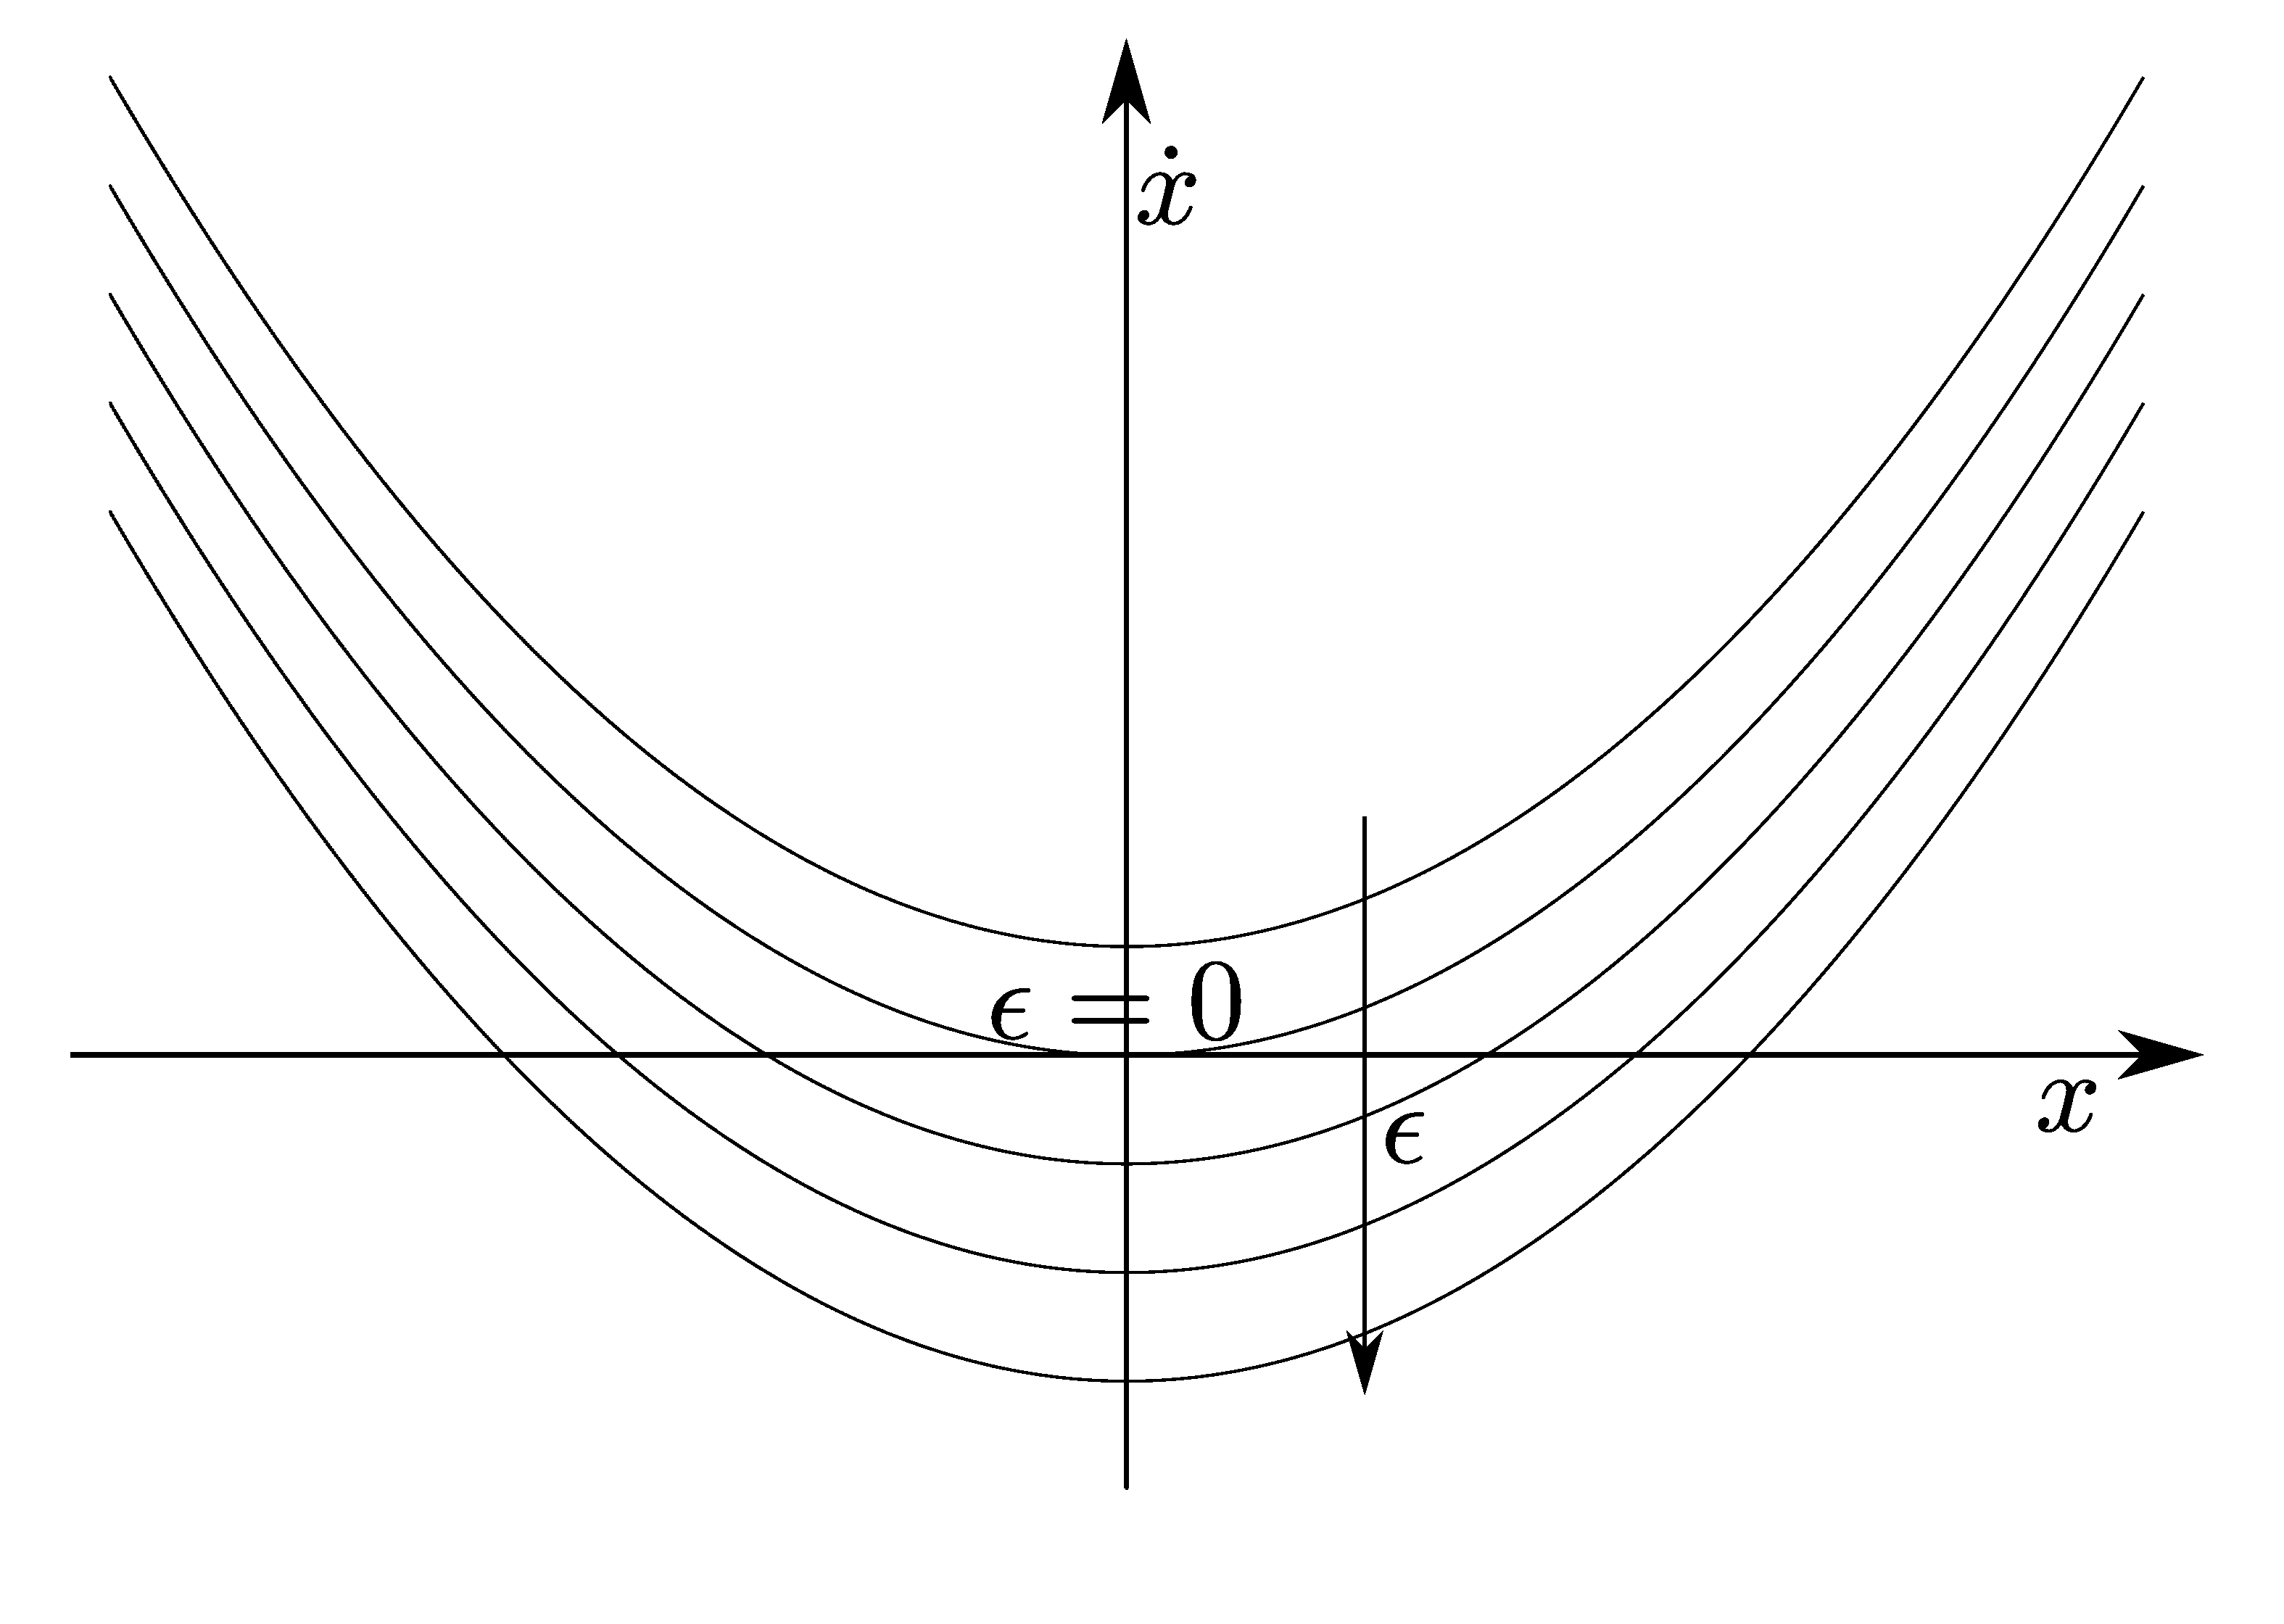
\includegraphics[width=0.5\textwidth]{images/epsilon=0}
\end{figure}





Attrattivo da sinistra e repulsivo da destra. \bigskip
Al lettore è lasciato risolvere esattamente per $\epsilon=0$ con dato iniziale qualsiasi $\tilde x \neq 0$ trovando il tempo di volo ad infinito.
\\
\textbf{Soluzione parziale/considerazioni}
\begin{figure}[H]
    \centering
  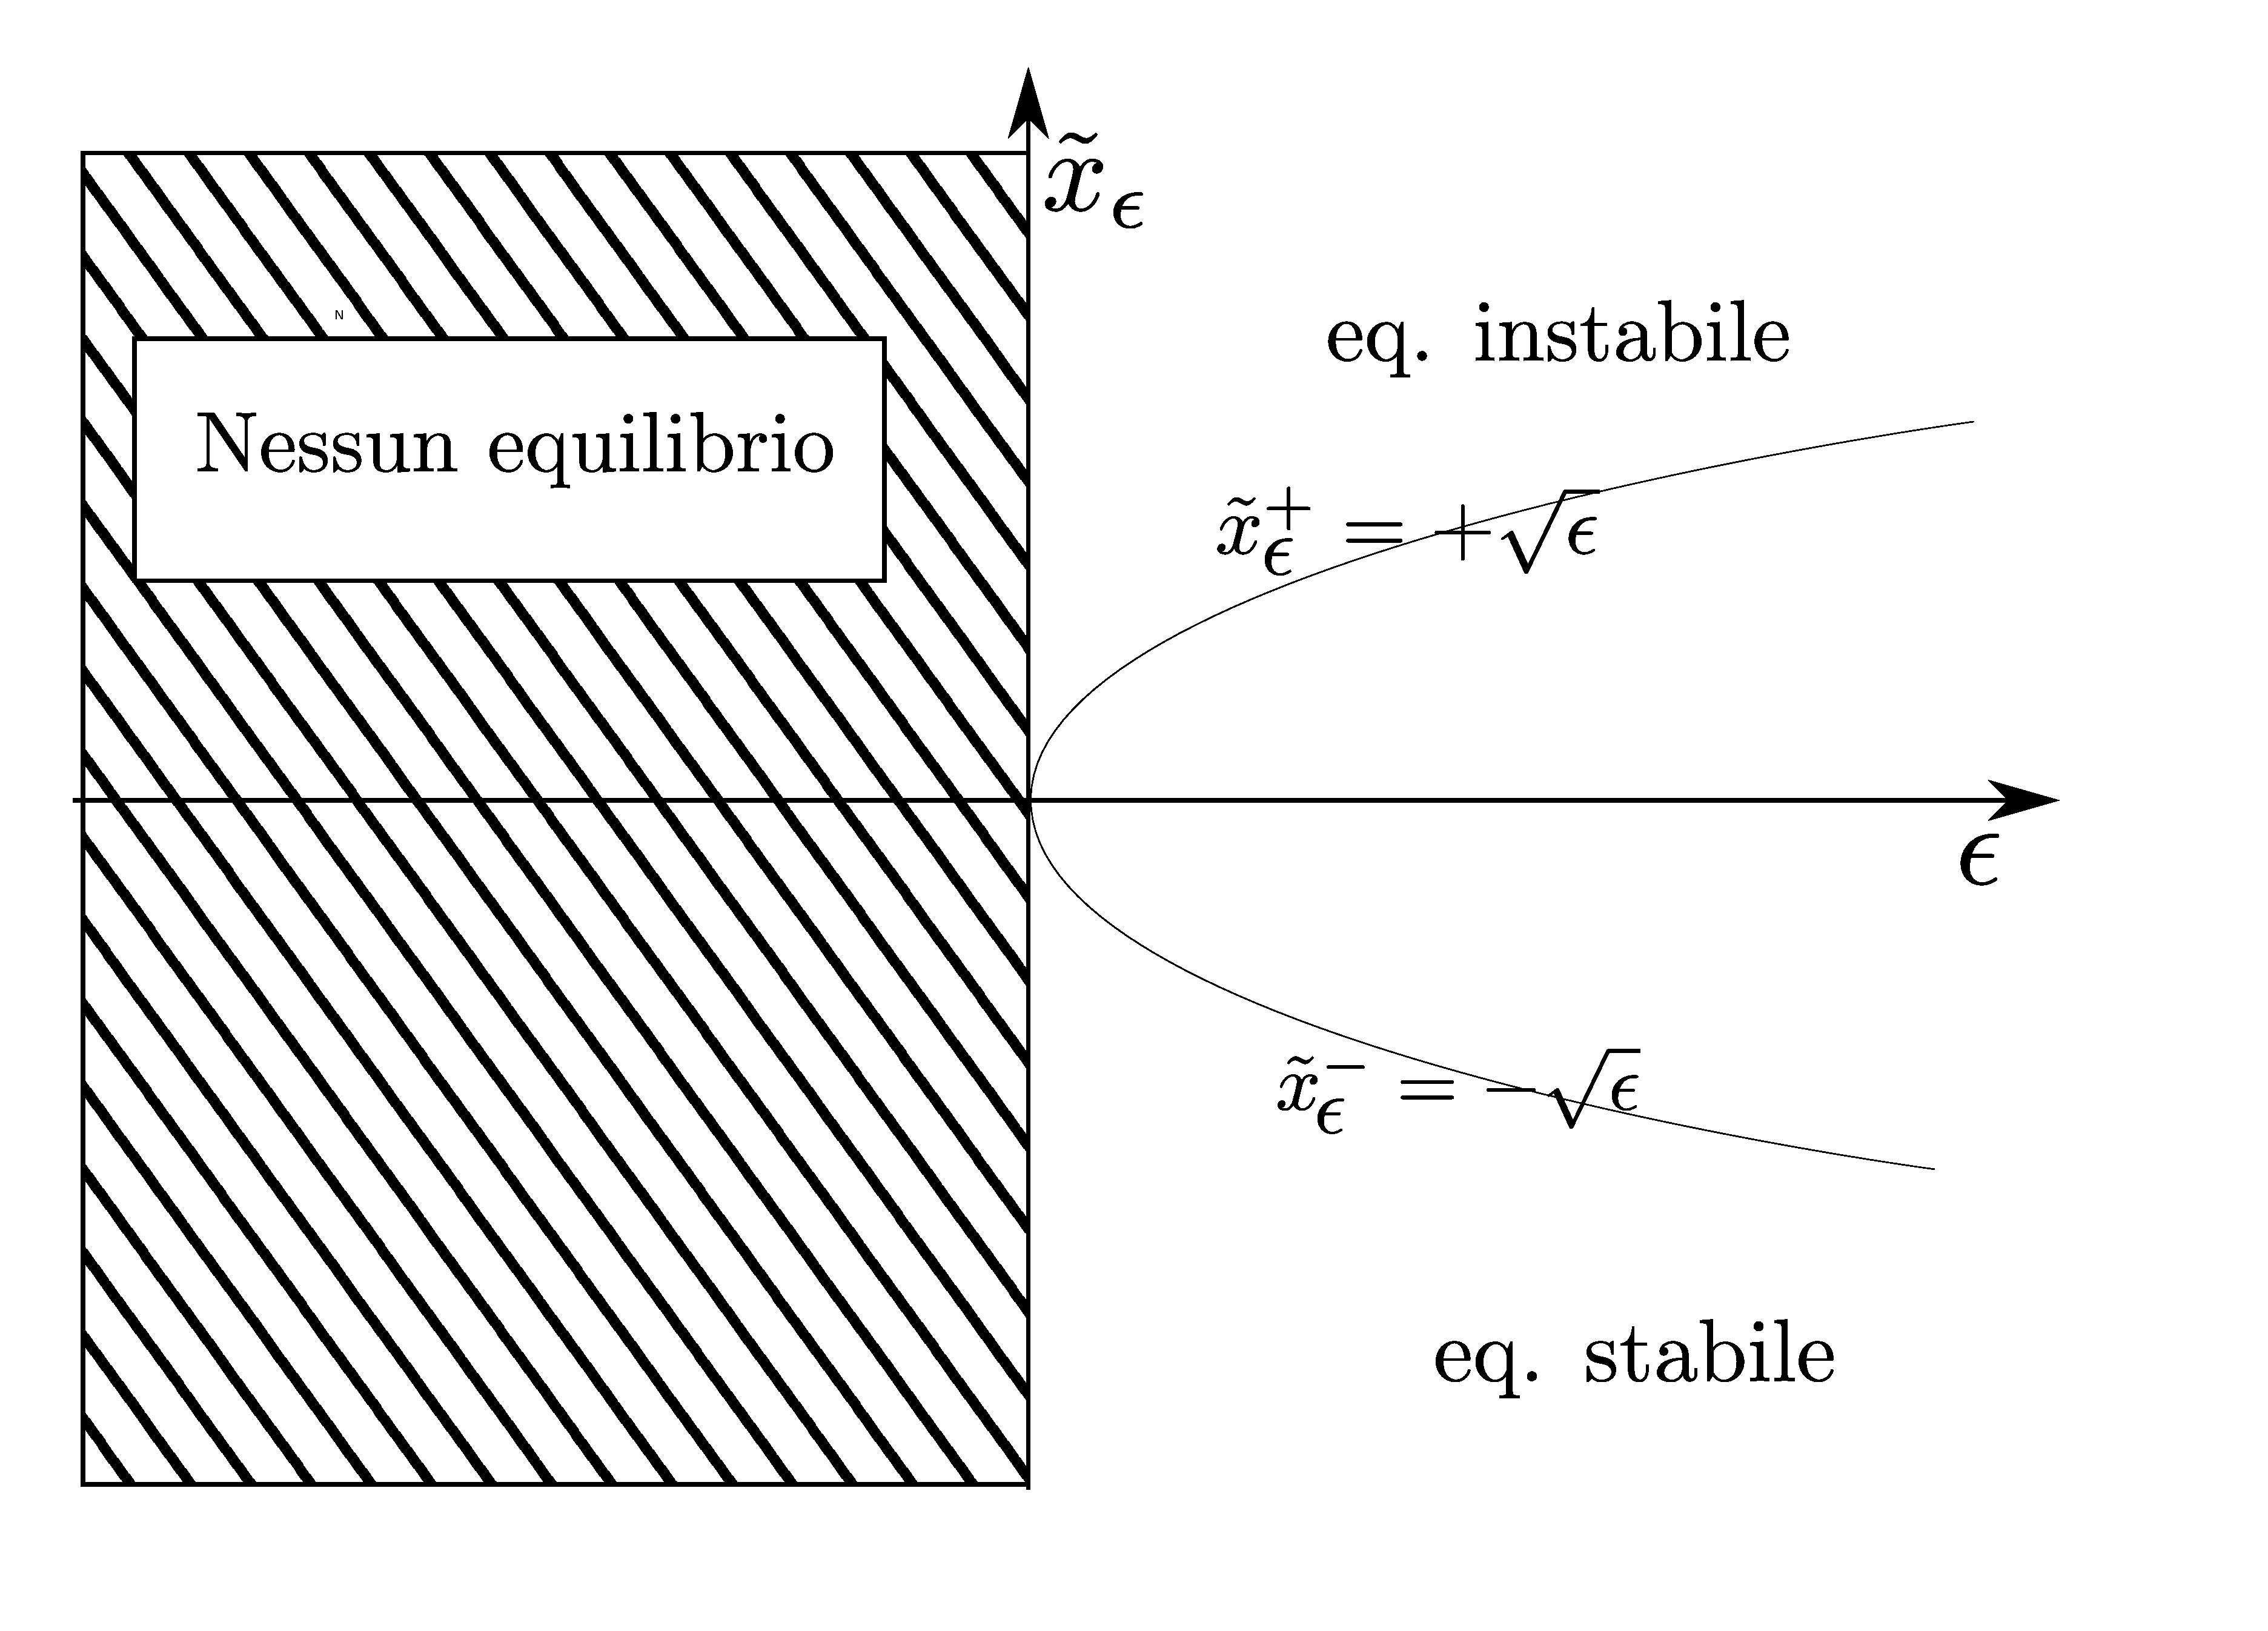
\includegraphics[width=0.5\textwidth]{images/diagrammadibiforcazione.pdf}
\end{figure}


Nel caso in cui $\epsilon \neq 0$ o non si ha soluzione: caso $\epsilon <0$ (non c'è intersezione con l'asse x) o ci sono due soluzioni una stabile/attrattiva e una instabile/repulsiva: caso $\epsilon >0$.

Le due soluzioni
$\tilde x ^ \pm _\epsilon = \pm \sqrt{\epsilon}$ si possono riassumere in un grafico con assi $\tilde x_\epsilon$ - $\epsilon$ in cui si nota che per $\epsilon<0$ non esistono soluzioni e per $\epsilon >0 $ esiste una soluzione instabile e una stabile. Attenzione che in un grafico come questo il sistema abita sull'asse y.	
\end{appendic}

\newpage
\begin{appendic}[Retta]
\begin{equation}
  \dot x = - x - \epsilon
\end{equation}

\begin{figure}[H]
    \centering
  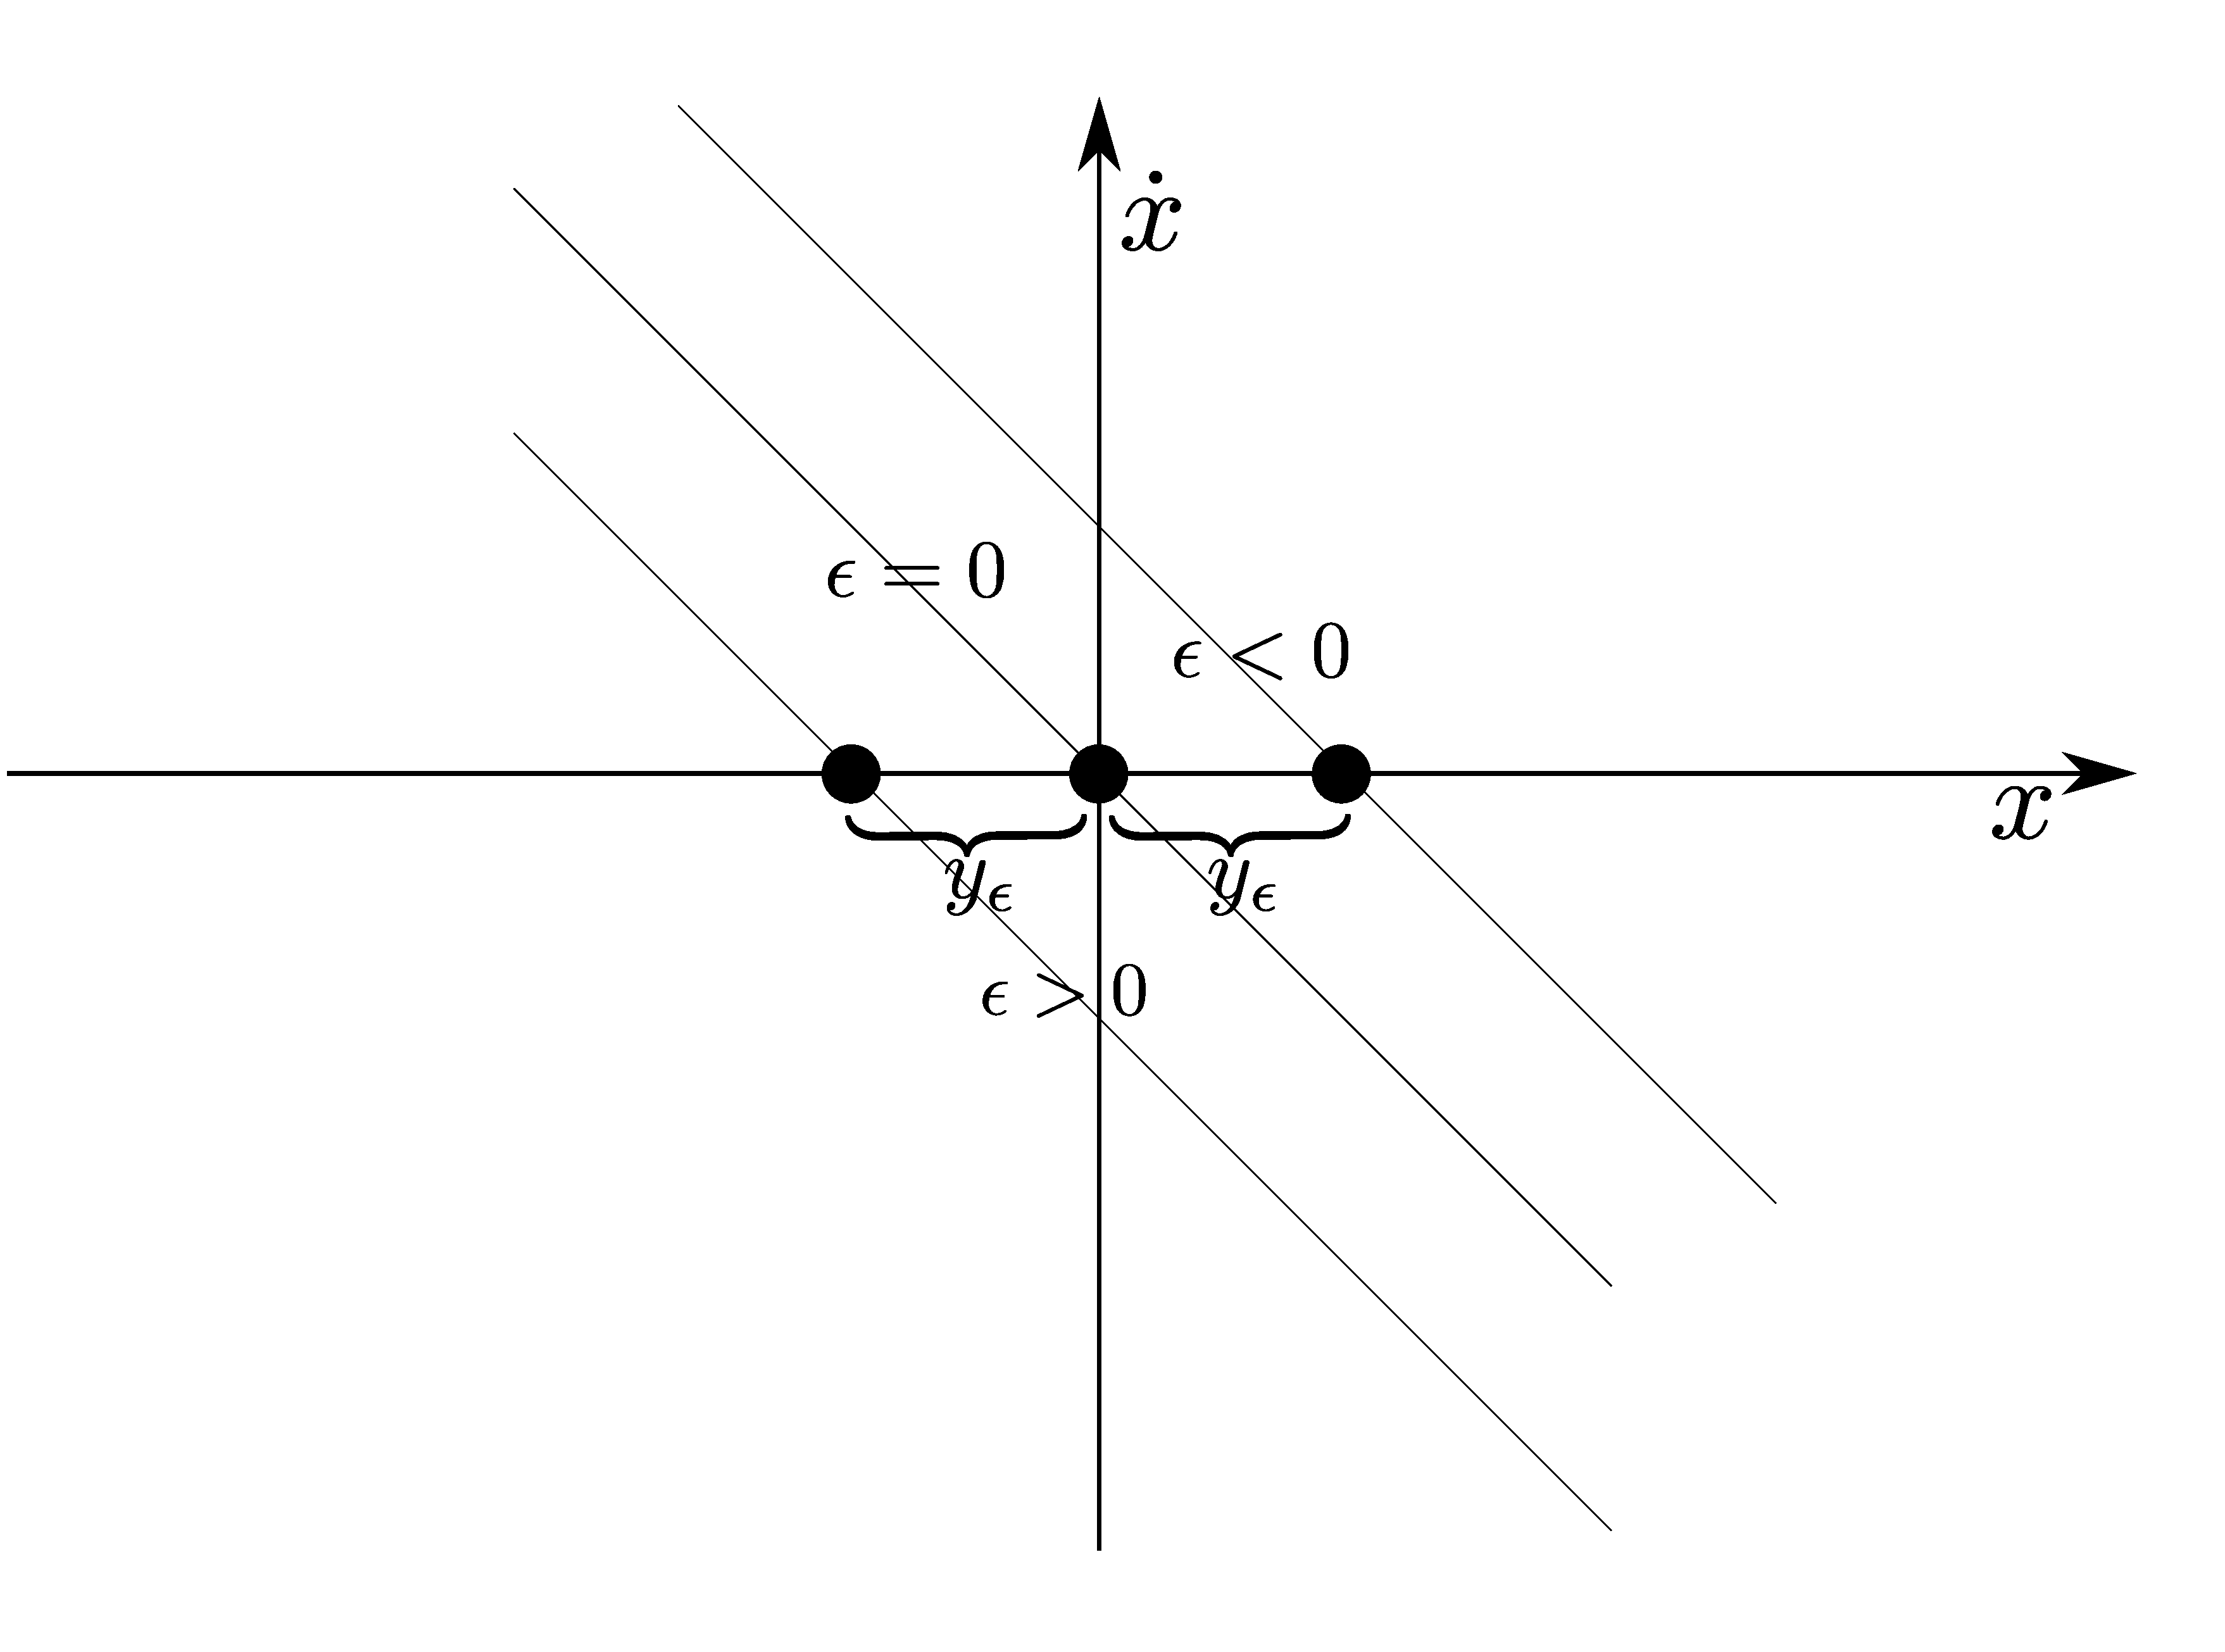
\includegraphics[width=0.6\textwidth]{images/campovett}
\end{figure}

Si vuole trovare lo spostamento degli equilibri per $\epsilon$ qualsiasi confrontandoli con il caso $\epsilon=0$ esplicitando la correzione degli stessi al primo ordine.\\
Considerando il campo $f(x)_\epsilon= f(x) - \epsilon$ si denota l'equilibrio semplice generico $\tilde x_\epsilon$ (funzione di $\epsilon$). Per $\epsilon$ piccoli $\tilde x_\epsilon$ sarà poco diverso da $\tilde x _0$: $\tilde x_\epsilon$=$\tilde x_0-y_\epsilon$; quindi considerando una $f(x)_\epsilon$ generica è possibile fare una linearizzazione (in questo caso non è necessario, essendo la funzione già lineare) permettendo di scrivere la differenza $y_\epsilon$. Infatti intanto vale
\begin{equation}
  0=f_\epsilon(\tilde x_\epsilon)=f_0(\tilde x_0-y_\epsilon)+\epsilon
\end{equation}
Ora sviluppando con Taylor:
\begin{equation}
  f_0(\tilde x_0)-\frac{d f}{dx}(\tilde x_0) \cdot y_\epsilon=-\epsilon
\end{equation}
Da qui utilizzando che $\tilde x_0$ è uno zero semplice si ha la seguente equazione importante valida per ogni funzione:
\begin{equation}
  y_\epsilon=\frac{\epsilon}{\frac{d f}{dx}(\tilde x_0)}
\end{equation}
In questo caso la derivata vale $1$, quindi tutti gli equilibri si spostano \textit{esattamente} di $-\epsilon$ (essendo la funzione $f(x)$ lineare l'approssimazione di Taylor è esatta).
\end{appendic}


\begin{appendic}[Potenziale di Morse]

\begin{equation}
  m \ddot x = - U'(x)
\end{equation}
in cui $U(x)$:

\begin{equation}
  U(x)= \frac{D}{2} (e^ {- \alpha x} -1)^2
\end{equation}

\begin{figure}[H]
    \centering
  \includegraphics[width=0.7\textwidth]{images/morse}
\end{figure}

Si può notare che per $x$ che tende a 0 $U(x)$ è approssimabile con una parabola:

\begin{equation}
  \lim_{x\rightarrow 0} \ \ \ \ U(x) \simeq \frac{D}{2} (\cancel{1} - \alpha x - \cancel{1})^2 = \frac{D}{2} \alpha^2 x^2 + o(x^3)
\end{equation}
Cioè la forza è praticamente lineare vicino a $x=0$, quindi il moto è oscillatorio semplice con frequenza (o meglio pulsazione) delle piccole oscillazioni intorno a 0 è $\omega = \sqrt{\frac{D \alpha^2}{m}}$.
\bigskip
\begin{osservazione} 
	Sviluppando l'espressione di $U$ si trova $\frac{D}{2} (e^{-2 \alpha x} - 2 e^{- \alpha x} +1)$. Il $+1$ è ininfluente sul diagramma di fase.
\end{osservazione}

\newpage \noindent 
\textbf{Diagramma di fase}
\newline
Riprendendo la conservazione dell'energia:

\begin{equation}
  \frac{mv^2}{2} = E-U(x)
\end{equation}
Quando $E= \frac{D}{2}$ si ha:
\begin{equation}
  v^2 = \frac{2}{m} \frac{D}{2}(1- (e^{- \alpha x}-1)^2)
\end{equation}
e 
\begin{equation}
  v(x)\xrightarrow{x\rightarrow + \infty}0
\end{equation}

Quando invece $E > \frac{D}{2}$ (alte energie):
\begin{equation}
  \frac{mv^2}{2} = E - \frac{D}{2} (e^{-\alpha x}-1)^2
\end{equation}
\begin{equation}
  \xrightarrow{x\rightarrow + \infty} E- \frac{D}{2}
\end{equation}
\begin{equation}
  v(x) \rightarrow \pm \sqrt{\frac{2}{m}(E - \frac{D}{2})}
\end{equation}


\begin{figure}[H]
    \centering
  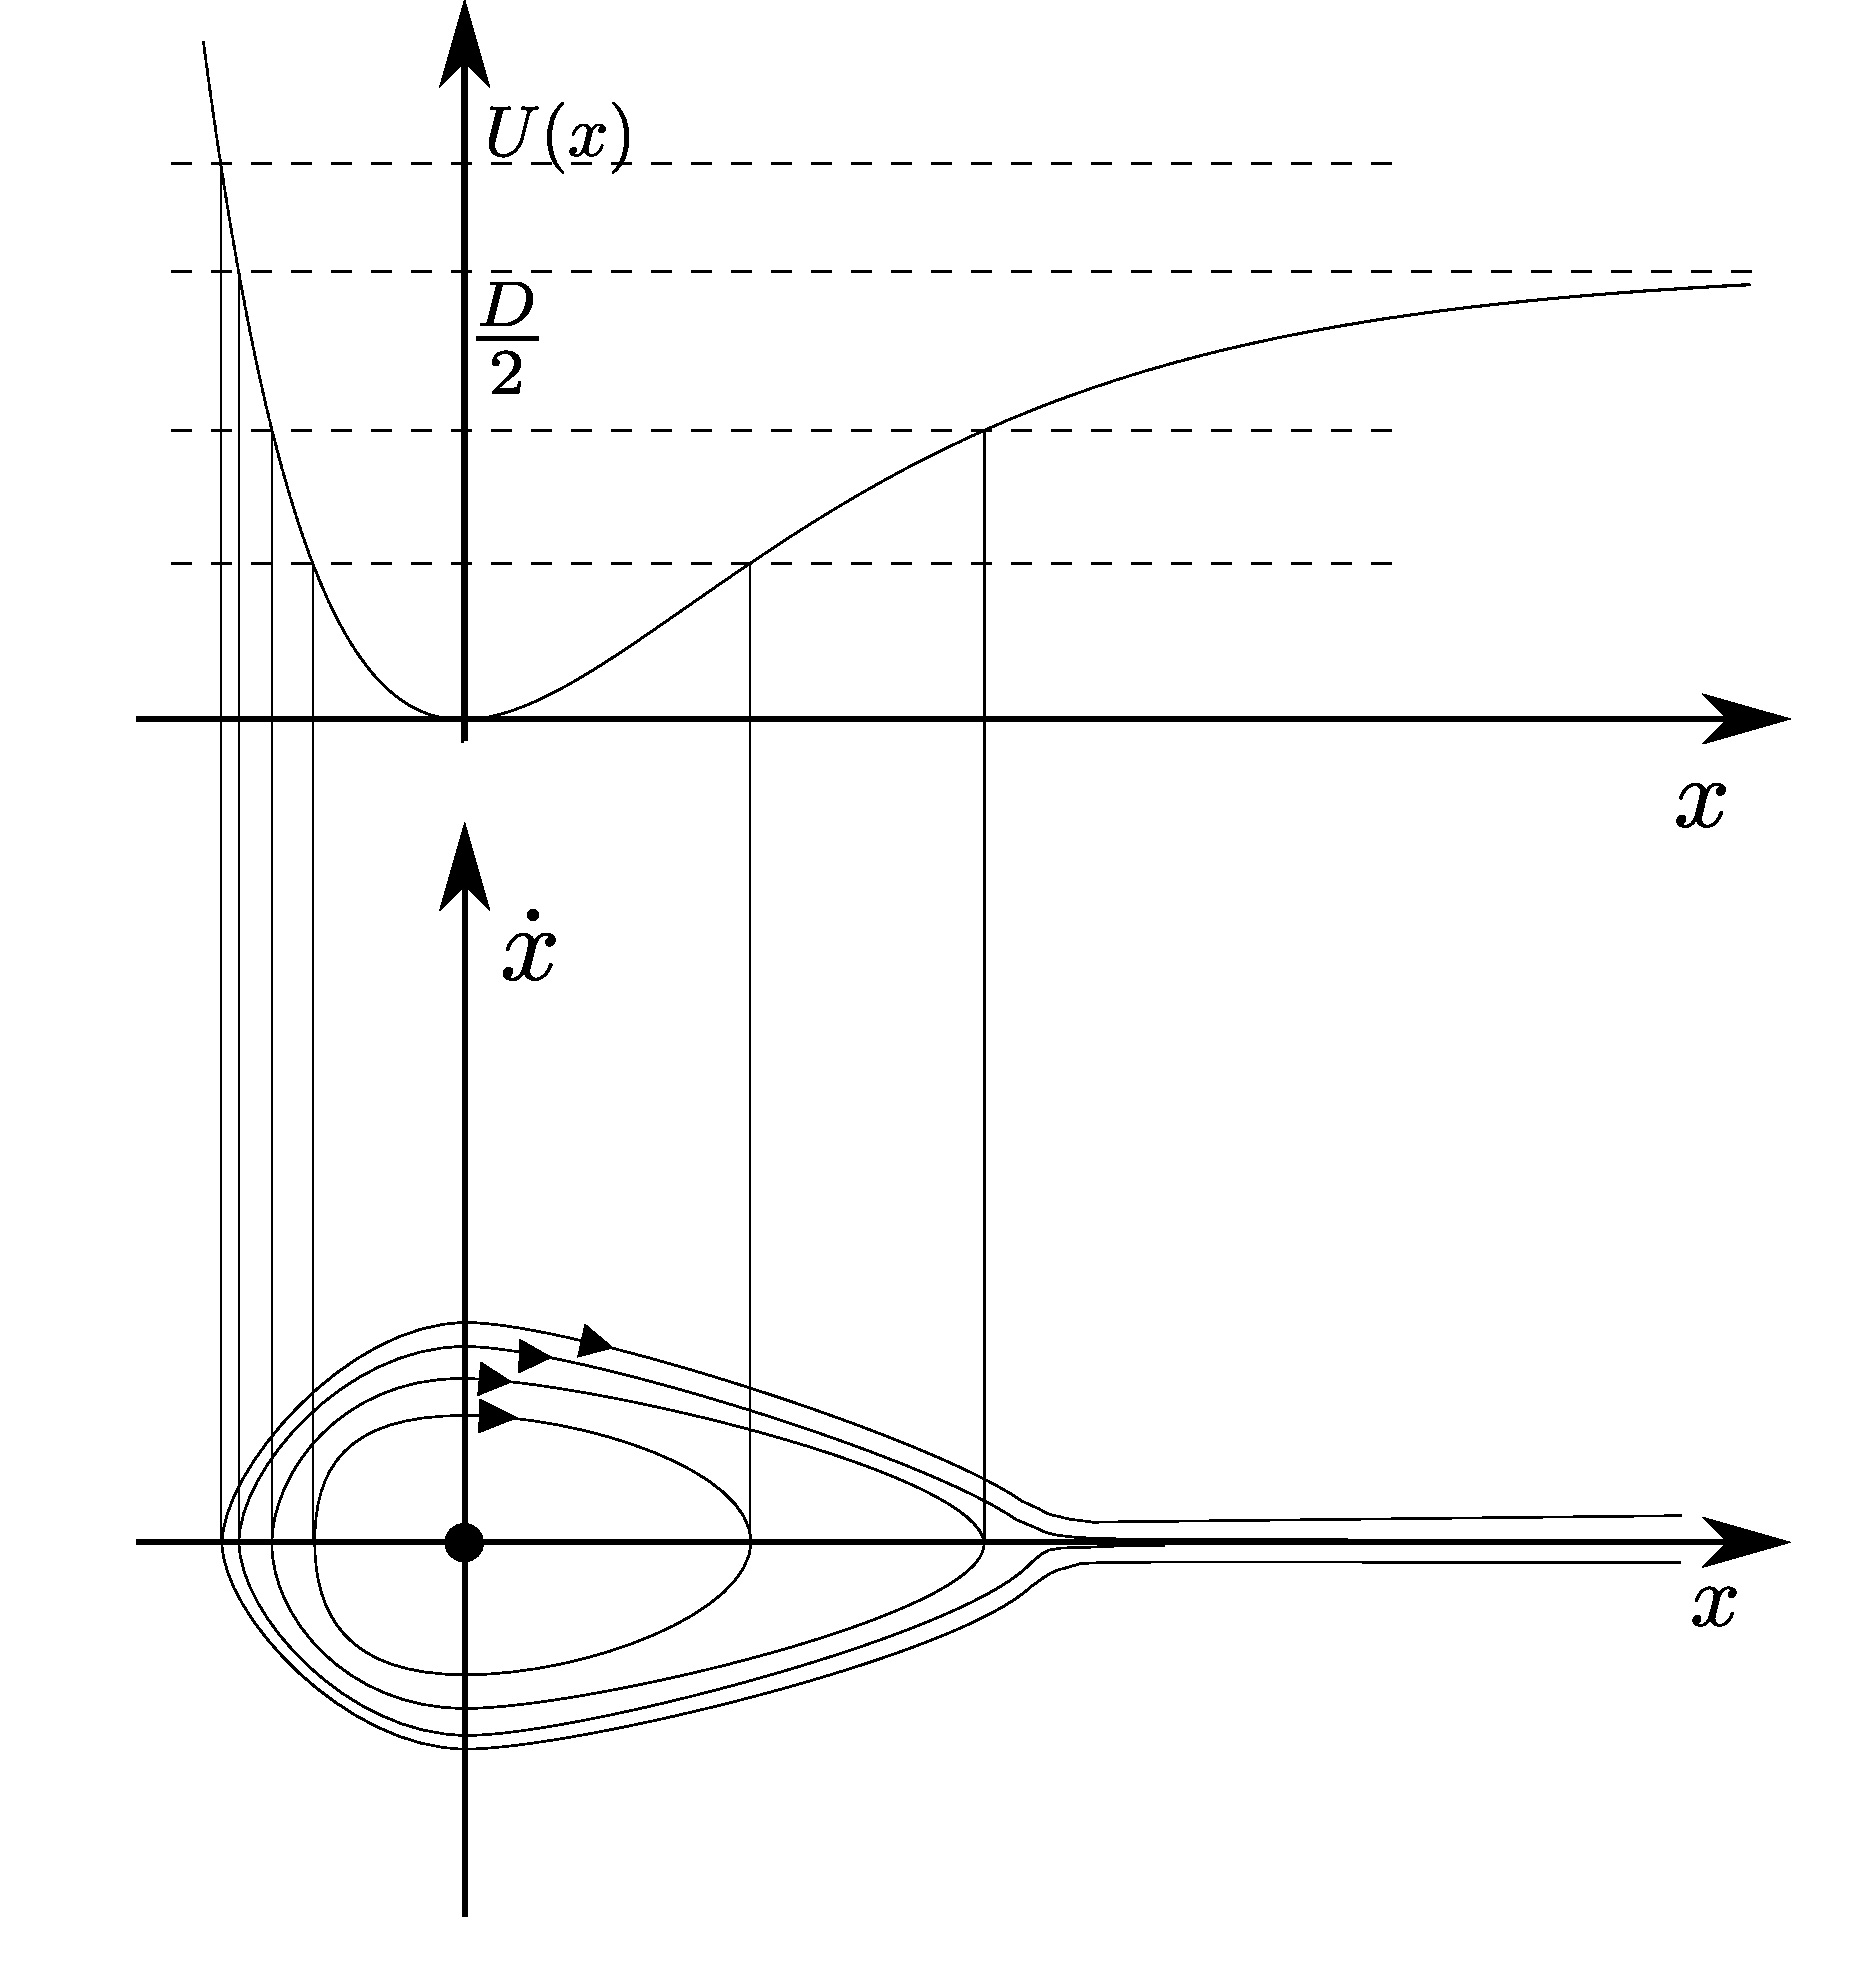
\includegraphics[width=0.662\textwidth]{images/uovo}
\end{figure}
\end{appendic}






\end{document}
